% MechanicsNumberedSolutionFigures20261023-v1
% MechanicsQualityRevision20261023-v1
% QualityRevision20261023
\begingroup
\tcbset{breakable/.default=false}
\chapter{合运动、抛体、圆周与一般曲线运动}

{
\graphicspath{{../../../sample/xes-original/kinematics-supplement/}{../../../sample/xes-original/kinematics-supplement/assets/}}
\section{运动的合成与分解}
\newcommand{\CoordinateSystemsDiagram}{%
\begin{center}\begin{tikzpicture}[scale=.9,>=Latex]
  \begin{scope}[xshift=-3.2cm]
    \draw[kaxis] (-2,0)--(2.2,0) node[right,clearlabel]{$x$};
    \draw[kaxis] (0,-1.7)--(0,1.9) node[above,clearlabel]{$y$};
    \coordinate (P) at (1.35,1.15);\node[point,label={[clearlabel]above:$P(x,y)$}] at (P) {};
    \draw[kguide] (P)--(1.35,0) (P)--(0,1.15);
    \node[below left] at (0,0){$O$};
  \end{scope}
  \begin{scope}[xshift=3.2cm]
    \draw[kaxis] (0,0)--(2.3,0) node[right,clearlabel]{$N$};
    \draw[kaxis] (0,0)--(0,1.9);
    \coordinate (P) at (1.45,1.25);\draw[vector] (0,0)--(P) node[midway,clearlabel,above left]{$r$};
    \node[point,label={[clearlabel]above:$P(r,\theta)$}] at (P) {};
    \draw[->,TextGray] (.65,0) arc[start angle=0,end angle=41,radius=.65];
    \node[clearlabel] at (.82,.28){$\theta$};
    \node[below left] at (0,0){$O$};
  \end{scope}
\end{tikzpicture}\figcap{平面直角坐标系与平面极坐标系。}\label{ch03:fig:k03-2-5}\end{center}}

\newcommand{\PathChoicesDiagram}{%
\begin{center}\begin{minipage}{.96\linewidth}\centering
\begin{tikzpicture}[scale=.9,>=Latex]
 \coordinate (A) at (0,0);\coordinate (B) at (8,1.5);
 \draw[kcurve] (A)--(B) node[pos=.72,above=3pt]{$P_1$};
 \draw[kcurve] (A)..controls (1,2.9) and (5.9,3.0)..(B) node[pos=.46,above=3pt]{$P_2$};
 \draw[kcurve] (A)..controls (1.3,1.4) and (2.1,1.65)..(3.2,.25)
 ..controls (5,-1.0) and (7.7,0)..(B);
 \draw[kcurve] (A)..controls (-2.5,4) and (3.6,4.3)..(3.0,-.1)
 ..controls (2.8,-1.8) and (8.9,-1.1)..(B);
 \draw[kcurve] (A)..controls (3.6,-2.4) and (8.8,-2.0)..(B);
 \node at (5,.3){$P_3$};\node at (.8,3.35){$P_4$};\node at (5.5,-1.85){$P_5$};
 \node[point,label=below left:$A$] at (A){};\node[point,label=above right:$B$] at (B){};
\end{tikzpicture}
\figcap{五条路径 $P_1,\ldots,P_5$ 均从 $A$ 到 $B$；路径不同，位移相同。}\label{ch03:fig:k03-2-6}
\end{minipage}\end{center}}

\newcommand{\DisplacementFanDiagram}{%
\begin{center}\begin{minipage}{.98\linewidth}\centering
\begin{tikzpicture}[scale=.95,>=Latex]
 \coordinate (A) at (0,0);
 \foreach \i in {1,...,10}{
  \pgfmathsetmacro{\xx}{.95*\i}\pgfmathsetmacro{\yy}{.8*\xx-.06*\xx*\xx}
  \draw[DeepBlue!60,->,thin] (A)--(\xx,\yy);
 }
 \draw[kcurve,domain=0:9.75,samples=100] plot (\x,{.8*\x-.06*\x*\x});
 \foreach \i in {1,...,10}{
  \pgfmathsetmacro{\xx}{.95*\i}\pgfmathsetmacro{\yy}{.8*\xx-.06*\xx*\xx}
  \node[point] at (\xx,\yy){};\node[above=5pt,font=\small] at (\xx,\yy){$B_{\i}$};
 }
 \node[point,label=below left:$A$] at (A){};
\end{tikzpicture}
\figcap{粗曲线是实际路径；从 $A$ 指向各 $B_i$ 的直箭头是对应位移。}\label{ch03:fig:k03-2-7}
\end{minipage}\end{center}}

\newcommand{\VectorOperationsDiagram}{%
\begin{center}\begin{tikzpicture}[scale=.82,>=Latex]
  \begin{scope}[xshift=-4.4cm]
    \draw[vector] (0,0)--(1.5,.35) node[midway,clearlabel,below]{$\vect A$};
    \draw[vector] (1.5,.35)--(2.15,1.55) node[midway,clearlabel,right]{$\vect B$};
    \draw[vector] (0,0)--(2.15,1.55) node[midway,clearlabel,above left]{$\vect A+\vect B$};
  \end{scope}
  \begin{scope}
    \draw[vector] (0,0)--(1.55,.4) node[midway,clearlabel,below]{$\vect A$};
    \draw[vector] (0,0)--(.55,1.55) node[midway,clearlabel,left]{$\vect B$};
    \draw[vector] (.55,1.55)--(1.55,.4) node[midway,clearlabel,above right]{$\vect A-\vect B$};
  \end{scope}
  \begin{scope}[xshift=4.4cm]
    \draw[vector] (0,0)--(1.7,.35) node[midway,clearlabel,below]{$\vect A$};
    \draw[vector] (0,0)--(.75,1.45) node[midway,clearlabel,left]{$\vect B$};
    \draw[->,TextGray] (.65,.13) arc[start angle=12,end angle=63,radius=.67];
    \node[clearlabel] at (.9,.75){$\theta$};
    \node[clearlabel,below] at (.85,-.55){$\vect A\cdot\vect B=AB\cos\theta$};
  \end{scope}
\end{tikzpicture}\figcap{矢量加法、减法与内积。}\label{ch03:fig:k03-2-8}\end{center}}

\newcommand{\VectorComponentsDiagram}{%
\begin{center}\begin{tikzpicture}[scale=.9,>=Latex]
  \draw[kaxis] (-.4,0)--(4.4,0) node[right,clearlabel]{$x$};
  \draw[kaxis] (0,-.35)--(0,3.0) node[above,clearlabel]{$y$};
  \coordinate (P) at (3.4,2.2);\draw[vector] (0,0)--(P) node[midway,clearlabel,above left]{$\vect A$};
  \draw[kguide] (P)--(3.4,0) node[clearlabel,below]{$A_x$};
  \draw[kguide] (P)--(0,2.2) node[clearlabel,left]{$A_y$};
\end{tikzpicture}\figcap{矢量平移到原点后，终点坐标就是矢量分量。}\label{ch03:fig:k03-2-9}\end{center}}

\newcommand{\CurveVelocityDiagram}{%
\begin{center}\begin{minipage}{.95\linewidth}\centering
\begin{tikzpicture}[>=Latex]
 \draw[kcurve,domain=-3:3,samples=100] plot (\x,{.09*\x^3-.55*\x});
 \foreach \xx in {-2.3,-.9,.8,2.2}{
  \pgfmathsetmacro{\yy}{.09*\xx^3-.55*\xx}
  \pgfmathsetmacro{\slope}{.27*(\xx)*(\xx)-.55}\pgfmathsetmacro{\dx}{1/sqrt(1+(\slope)*(\slope))}
  \node[point] at (\xx,\yy){};\draw[vector] (\xx,\yy)--++(\dx,{\slope*\dx});
 }
\end{tikzpicture}
\figcap{每个速度箭头都从所在位置出发，并沿该点的轨迹切线。}\label{ch03:fig:k03-2-10}
\end{minipage}\end{center}}

\newcommand{\AccelerationVectorDiagram}{%
\begin{center}\begin{tikzpicture}[scale=.9,>=Latex]
  \coordinate (O) at (0,0);\coordinate (A) at (2.3,1.6);\coordinate (B) at (3.2,.75);
  \draw[vector] (O)--(A) node[midway,clearlabel,above left]{$\vect v(t)$};
  \draw[vector] (O)--(B) node[midway,clearlabel,below=7pt]{$\vect v(t+\Delta t)$};
  \draw[vector] (A)--(B) node[midway,clearlabel,above right]{$\Delta\vect v$};
  \node[clearlabel,right] at (3.65,1.2){$\displaystyle \vect a=\lim_{\Delta t\to0}\frac{\Delta\vect v}{\Delta t}$};
\end{tikzpicture}\figcap{速度矢量首端重合，终端之差给出 $\Delta\vect v$。}\label{ch03:fig:k03-2-11}\end{center}}

\newcommand{\RescueRouteDiagram}{%
\begin{center}\begin{minipage}{.96\linewidth}\centering
\begin{tikzpicture}[>=Latex]
 \coordinate (A) at (-2.8,2.3);\coordinate (C) at (.2,0);\coordinate (B) at (1.7,-1.9);
 \coordinate (U) at (.2,1.4);\coordinate (D) at (.2,-1.4);
 \draw[thick] (-3.5,0)--(3.6,0) node[right]{岸线};
 \draw[kguide] (A)--(-2.8,0) (B)--(1.7,0) (U)--(D);
 \draw[vector] (A)--(C) node[pos=.35,above right=2pt]{$v_1$};
 \draw[vector] (C)--(B) node[pos=.45,above right=2pt]{$v_2$};
 \draw pic[draw=TextGray,angle radius=7mm] {angle=U--C--A};
 \draw pic[draw=TextGray,angle radius=7mm] {angle=D--C--B};
 \node at (-.24,1.03){$\theta_1$};\node at (.55,-1.1){$\theta_2$};
 \draw[<->,TextGray] (-3.3,0)--(-3.3,2.3) node[midway,left]{$d_1$};
 \draw[<->,TextGray] (2.15,0)--(2.15,-1.9) node[midway,right]{$d_2$};
 \draw[<->,TextGray] (-2.8,-2.5)--(.2,-2.5) node[midway,below]{$x$};
 \draw[<->,TextGray] (.2,-2.5)--(1.7,-2.5) node[midway,below]{$L-x$};
 \node[point,label=above left:$A$] at (A){};\node[point,label=below right:$B$] at (B){};
 \node[point,label=above right:$C$] at (C){};
\end{tikzpicture}
\figcap{入水点为 $C$；$\theta_1,\theta_2$ 从岸线法线量起，两垂足间距为 $L$。}\label{ch03:fig:k03-ex-2-31}
\end{minipage}\end{center}}

\newcommand{\FootballInterceptionDiagram}{%
\begin{center}\begin{minipage}{.96\linewidth}\centering
\begin{tikzpicture}[scale=1.1,>=Latex]
 \coordinate (A) at (0,0);\coordinate (B) at (4,2);\coordinate (C) at (5,0);\coordinate (X) at (6,0);
 \draw[kaxis] (A)--(X) node[right]{$X$};
 \draw[thick] (A)--(B) node[midway,above left]{$d$};\draw[kguide] (B)--(C);
 \draw[vector] (B)--($(B)!.43!(C)$) node[midway,right=5pt]{$\vect v_p$};
 \draw[vector] (A)--(1.25,0) node[midway,below=4pt]{$\vect v$};
 \draw pic[draw=TextGray,angle radius=8mm] {angle=X--A--B};\node at (1.03,.27){$\theta$};
 \draw pic[draw=TextGray,angle radius=4mm] {right angle=A--B--C};
 \foreach \p/\pos in {A/below left,B/above,C/below}\node[point,label=\pos:$\p$] at (\p){};
\end{tikzpicture}
\figcap{最低奔跑速率对应 $BC\perp AB$；队员速度沿 $BC$，球的速度沿 $AC$。}\label{ch03:fig:k03-ex-2-29}
\end{minipage}\end{center}}

\newcommand{\TwoParticlesMinimumDistanceDiagram}{%
\begin{center}\begin{tikzpicture}[scale=.82,>=Latex]
  \coordinate (P) at (-3.7,-.75);\coordinate (Q) at (2.25,-.75);\coordinate (R) at (-.3,2.25);
  \draw[very thick] (P)--(Q);
  \draw[kguide] (Q)--(R);
  \draw[vector] (-3.25,-.75)--(-1.8,-.75) node[midway,clearlabel,above]{$\vect v_1$};
  \draw[vector] (1.93,-.38)--(.95,.78) node[midway,clearlabel,right]{$\vect v_2$};
  \draw pic[draw=TextGray,->,angle radius=8mm,"$\alpha$"{clearlabel}] {angle=R--Q--P};
  \draw[<->,TextGray] (P)--(Q) node[midway,clearlabel,below=3pt]{$l$};
  \node[point,label={[clearlabel]left:$A,P$}] at (P) {};
  \node[point,label={[clearlabel]right:$B,Q$}] at (Q) {};
  \node[clearlabel,above] at (R){$R$};
\end{tikzpicture}\figcap{初始连线为 $PQ$；$A$ 沿 $PQ$，$B$ 沿 $QR$，最近距离由相对速度直线确定。}\label{ch03:fig:k03-ex-2-30}\end{center}}

\newcommand{\KQuestionAW}{%
\begin{center}\begin{minipage}{.97\linewidth}\centering
\begin{tikzpicture}[>=Latex,scale=.70]

\foreach \x in {-4,-3,-2,-1,1,2,3,4,5}{\draw[RuleGray,thin] (\x,-5.5)--(\x,-.8) (\x,.1)--(\x,5);}
\foreach \y in {-5,-4,-3,-2,-1,1,2,3,4,5}{\draw[RuleGray,thin] (-4,\y)--(-1.05,\y) (.12,\y)--(5.5,\y);}
\draw[kaxis] (-4.2,0)--(5.8,0) node[right]{$x$};
\draw[kaxis] (0,-5.7)--(0,5.3) node[above]{$y$};
\foreach \x in {-3,-2,-1,1,2,3,4,5}\node[below=2pt] at (\x,0){$\x$};
\foreach \y in {-5,-4,-3,-2,-1,1,2,3,4}\node[left=2pt] at (0,\y){$\y$};
\node[above left=3pt] at (0,0){$O$};

\end{tikzpicture}
\figcap{题图：在直角坐标网格中标出题设各点。}\label{ch03:ref:question-figure-2-22}
\end{minipage}\end{center}
}

\newcommand{\KQuestionAX}{%
\begin{center}\begin{minipage}{.97\linewidth}\centering
\begin{tikzpicture}[>=Latex,scale=.9]

\draw[kaxis] (0,0)--(6,0) node[right]{$r$};
\foreach \r in {1,...,5}{\draw (\r,0)--(\r,.1);\node[below] at (\r,0){$\r$};}
\node[left] at (0,0){$O$};
\path[use as bounding box] (-.5,-1.4) rectangle (6.4,1.4);

\end{tikzpicture}
\figcap{题图：以向右射线为极轴，逆时针为正角方向。}\label{ch03:ref:question-figure-2-23}
\end{minipage}\end{center}
}

\newcommand{\KQuestionBC}{%
\begin{center}\begin{minipage}{.97\linewidth}\centering
\begin{tikzpicture}[>=Latex,scale=.9]

\coordinate (A) at (3,0);\coordinate (M) at (0,3);\coordinate (N) at (6,3);
\coordinate (B) at (1.125,3);\coordinate (H) at (3,3);
\draw[kguide] (M)--(N) (A)--(H) (A)--(B);
\node[point,label=below:$A$] at (A){};
\node[left] at (M){$M$};\node[right] at (N){$N$};
\draw[vector] (B)--++(1.1,0) node[midway,above]{$v$};
\draw[vector] (A)--++(0,1.7) node[midway,right]{$u$};
\node[below left] at (B){$B$};\node[above right] at (H){$H$};
\draw[TextGray] (A)++(90:.8) arc(90:122:.8);\node at (2.64,1.13){$\theta$};
\draw[<->] (3.7,0)--(3.7,3) node[midway,right]{$L$};

\end{tikzpicture}
\figcap{题图：潜艇 A 与航线 MN 的垂直距离为 $L$，$\theta$ 从航线法线量起。}\label{ch03:ref:question-figure-2-28}
\end{minipage}\end{center}
}

\newcommand{\KQuestionBD}{%
\begin{center}\begin{minipage}{.97\linewidth}\centering
\begin{tikzpicture}[>=Latex,scale=.9]

\coordinate (A) at (0,0);\coordinate (B) at (4,2);\coordinate (X) at (6,0);
\draw[kaxis] (A)--(X) node[right]{$X$};\draw[thick] (A)--(B) node[midway,above left]{$d$};
\draw[vector] (A)--(1.3,0) node[midway,below]{$v$};
\draw[vector] (B)--++(.5,-1.1) node[right]{$v_p$};
\draw (0.8,0) arc(0:26.565:.8);\node at (1.12,.3){$\theta$};
\node[point,label=below left:$A$] at (A){};\node[point,label=above:$B$] at (B){};

\end{tikzpicture}
\figcap{题图：球沿 AX 运动，队员从 B 开始奔跑；奔跑方向待选。}\label{ch03:ref:question-figure-2-29}
\end{minipage}\end{center}
}

\newcommand{\KQuestionBE}{%
%
\begin{center}\begin{tikzpicture}[scale=.82,>=Latex]
  \coordinate (P) at (-3.7,-.75);\coordinate (Q) at (2.25,-.75);\coordinate (R) at (-.3,2.25);
  \draw[very thick] (P)--(Q);
  \draw[kguide] (Q)--(R);
  \draw[vector] (-3.25,-.75)--(-1.8,-.75) node[midway,clearlabel,above]{$\vect v_1$};
  \draw[vector] (1.93,-.38)--(.95,.78) node[midway,clearlabel,right]{$\vect v_2$};
  \draw pic[draw=TextGray,->,angle radius=8mm,"$\alpha$"{clearlabel}] {angle=R--Q--P};
  \draw[<->,TextGray] (P)--(Q) node[midway,clearlabel,below=3pt]{$l$};
  \node[point,label={[clearlabel]left:$A,P$}] at (P) {};
  \node[point,label={[clearlabel]right:$B,Q$}] at (Q) {};
  \node[clearlabel,above] at (R){$R$};
\end{tikzpicture}\figcap{题图：A、B 初始位于 P、Q，分别沿 PQ、QR 匀速运动。}\label{ch03:ref:question-figure-2-30}\end{center}
}

\newcommand{\KQuestionBF}{%
%
\begin{center}\begin{minipage}{.96\linewidth}\centering
\begin{tikzpicture}[>=Latex]
 \coordinate (A) at (-2.8,2.3);\coordinate (C) at (.2,0);\coordinate (B) at (1.7,-1.9);
 \coordinate (U) at (.2,1.4);\coordinate (D) at (.2,-1.4);
 \draw[thick] (-3.5,0)--(3.6,0) node[right]{岸线};
 \draw[kguide] (A)--(-2.8,0) (B)--(1.7,0) (U)--(D);
 \draw[vector] (A)--(C) node[pos=.35,above right=2pt]{$v_1$};
 \draw[vector] (C)--(B) node[pos=.45,above right=2pt]{$v_2$};
 \draw pic[draw=TextGray,angle radius=7mm] {angle=U--C--A};
 \draw pic[draw=TextGray,angle radius=7mm] {angle=D--C--B};
 \node at (-.24,1.03){$\theta_1$};\node at (.55,-1.1){$\theta_2$};
 \draw[<->,TextGray] (-3.3,0)--(-3.3,2.3) node[midway,left]{$d_1$};
 \draw[<->,TextGray] (2.15,0)--(2.15,-1.9) node[midway,right]{$d_2$};
 \draw[<->,TextGray] (-2.8,-2.5)--(.2,-2.5) node[midway,below]{$x$};
 \draw[<->,TextGray] (.2,-2.5)--(1.7,-2.5) node[midway,below]{$L-x$};
 \node[point,label=above left:$A$] at (A){};\node[point,label=below right:$B$] at (B){};
 \node[point,label=above right:$C$] at (C){};
\node[below left=3pt] at (-3.5,0){$M$};\node[above left=6pt] at (3.6,0){$N$};
\end{tikzpicture}
\figcap{题图：A 在岸上、B 在水中，C 为待选择的入水点；两垂足间距为 $L$。}\label{ch03:ref:question-figure-2-31}
\end{minipage}\end{center}
}


一维运动只需一个坐标。质点在平面或空间中运动时，位置、位移、速度和加速度都需要同时包含多个方向的信息。多数常见运动先可限制在一个平面内讨论；掌握二维情况后，只需增加第三个分量即可推广到三维。

这里的困难并不只是“多写一个坐标”。在直线上，正、负两个方向已经由数轴规定；到了平面内，同样大小的位移可以指向无穷多个方向，速度的大小不变时方向也可能不断改变。因此，描述平面运动必须把“大小”和“方向”同时纳入运算。抛体、车辆转弯和行星绕中心运动都属于这一类问题，它们虽然轨迹不同，却可以用同一套坐标、矢量和分量方法处理。

\subsection{位置的确定：坐标系}

平面直角坐标系由原点 $O$ 和两条互相垂直、带正方向的坐标轴组成，点 $P$ 由 $(x,y)$ 唯一确定。平面极坐标系由极点 $O$、参考方向 $ON$ 和坐标 $(r,\theta)$ 组成，其中 $r\ge0$；角度相差 $2\pi$ 的整数倍表示同一点，且 $r=0$ 时角度没有实际意义。

日常语言里也常用这两种定位思路。例如“从某地向西若干千米、再向北若干千米”对应直角坐标分量；“位于某地北偏西某角度、距离若干千米”对应极坐标。直角坐标中的 $x<0$ 只说明点在 $y$ 轴左侧，$y<0$ 只说明点在 $x$ 轴下方；极坐标中的 $r$ 是距离，通常取非负值，而 $\theta$ 的零方向和正向必须事先约定。

\CoordinateSystemsDiagram

坐标系必须在列方程前说明。直角坐标适合方向固定或边界平直的问题；极坐标适合具有明显中心的运动，如行星公转和圆周运动。坐标系不同不会改变实际运动，但会改变分量表达式的复杂程度。

完整的坐标系约定至少包括原点位置、各轴正方向和单位；极坐标还必须说明参考射线及角度正向。只有这些信息给全，$(x,y)$ 或 $(r,\theta)$ 才能被还原为唯一的空间位置。选择坐标系具有任意性，却不是随意性：同一问题可以有许多合法选法，其中与边界、运动方向或对称中心一致的选法往往使后续方程最简单。

两种坐标表示可以互相转换。在约定 $x$ 轴正向为极角零方向、逆时针为正时，
\begin{equation}
 x=r\cos\theta,\qquad y=r\sin\theta,\qquad
 r=\sqrt{x^2+y^2}.
\end{equation}
由 $x,y$ 求 $\theta$ 时要根据象限确定，而不能只使用 $\arctan(y/x)$ 的主值。极点处 $r=0$，所有角度都给出同一点，所以此处的 $\theta$ 不可由位置唯一确定。这种坐标奇点是表示方法的特点，不是实际空间出现了异常。

直角坐标适合分量方向固定的问题，极坐标适合“离中心多远、绕中心转了多少”的问题。例如同一圆周在直角坐标中需写 $x^2+y^2=R^2$，在极坐标中只需写 $r=R$；但匀速直线运动若不通过极点，用极坐标表示反而可能更复杂。选系的标准是让约束和运动规律尽量简单，而不是固定偏爱某一种。

\begin{origexamplebox}{在直角坐标系中标点}\label{ch03:ex:k03-2-22}
在平面直角坐标系中标出
\[
A(3,4),\ B(5,0),\ C(-3,2),\ D(2,-5),\ E(-3,-2),\ F(0,3),\ G(-1,0),\ H(0,-3).
\]
\par 题图见图~\ref{ch03:ref:question-figure-2-22}。
\KQuestionAW
\end{origexamplebox}
\Needspace{6\baselineskip}\begin{xesolution}
以下推导所用的解图为图~\ref{mech:legacy:ch03:k03-2-22}。

横坐标决定左右，纵坐标决定上下；坐标为零表示点在相应坐标轴上。图中 $A,C,E,D$ 分别位于第一、第二、第三、第四象限，$B,G$ 在 $x$ 轴上，$F,H$ 在 $y$ 轴上。
\begin{center}\begin{qualityfigure}
\begin{tikzpicture}[scale=.52]
\draw[kaxis] (-5.8,0)--(5.8,0) node[right,clearlabel]{$x$};\draw[kaxis] (0,-5.8)--(0,5.8) node[above,clearlabel]{$y$};
\draw[step=1,RuleGray!65,thin] (-5,-5) grid (5,5);
\foreach \name/\x/\y/\pos in {A/3/4/above,B/5/0/above,C/-3/2/above,D/2/-5/below,E/-3/-2/below,F/0/3/right,G/-1/0/below,H/0/-3/right}{\node[point,label={[clearlabel]\pos:$\name$}] at (\x,\y) {};}
\end{tikzpicture}
\figcap{本题解答中的位置、分量与辅助量。}\label{mech:legacy:ch03:k03-2-22}
\end{qualityfigure}\end{center}
\end{xesolution}


\begin{origexamplebox}{在极坐标系中标点}\label{ch03:ex:k03-2-23}
在平面极坐标系中标出
\[
A(5,\pi/3),\ B(2,\pi/3),\ C(5,\pi/2),\ D(4,\pi),\ E(4,3\pi/2),\ F(3,0).
\]
\par 题图见图~\ref{ch03:ref:question-figure-2-23}。
\KQuestionAX
\end{origexamplebox}
\Needspace{6\baselineskip}\begin{xesolution}
以下推导所用的解图为图~\ref{mech:legacy:ch03:k03-2-23}。

先约定从正 $x$ 轴逆时针量角，再按角度画射线，沿射线量取半径。
$A,B$ 都在 $60^\circ$ 射线上，距原点分别为 $5,2$。
$C$ 的极角为 $\pi/2=90^\circ$，在正 $y$ 轴；$E$ 的极角为 $3\pi/2=270^\circ$，在负 $y$ 轴。
$D$ 在负 $x$ 轴，$F$ 在正 $x$ 轴。也可用 $y_C=5\sin(\pi/2)=5$ 检查 $C$ 的上下位置。
\begin{center}\begin{qualityfigure}
\begin{tikzpicture}[scale=.55]
\draw[kaxis] (-5.8,0)--(5.8,0) node[right,clearlabel]{$x$};\draw[kaxis] (0,-5.8)--(0,5.8) node[above,clearlabel]{$y$};
\foreach \r in {1,...,5}{\draw[RuleGray] (0,0) circle (\r);}
\foreach \name/\r/\a/\pos in {A/5/60/above,B/2/60/above,C/5/90/right,D/4/180/above,E/4/270/left,F/3/0/above}{\node[point,label={[clearlabel]\pos:$\name$}] at (\a:\r) {};}
\end{tikzpicture}
\figcap{本题解答中的位置、分量与辅助量。}\label{mech:legacy:ch03:k03-2-23}
\end{qualityfigure}\end{center}
\end{xesolution}

\subsection{位移、矢量及其分量}

质点从起点到终点的\textbf{位移}是由起点指向终点的有向线段。位移只依赖始末位置，路程则依赖实际轨迹。沿曲线前进一小段时，位移大小与路程之差是高阶小量；经过较长路程后，两者可能相差很大。

因此，给定初位置和一段过程的位移就能唯一确定末位置，却不能由此还原质点实际经过的道路。反过来，即使两次运动的轨迹完全不同，只要起点和终点相同，它们的位移就相同。把初、末坐标写成 $(x_1,y_1)$ 与 $(x_2,y_2)$，坐标增量 $\Delta x=x_2-x_1$、$\Delta y=y_2-y_1$ 正好给出位移在两轴上的分量。

\PathChoicesDiagram

图~\ref{ch03:fig:k03-2-6}中的五条路径具有相同的起点 $A$ 和终点 $B$，却给出不同路程；图~\ref{ch03:fig:k03-2-7}中的每根箭头都从同一初始点 $A$ 指向一个时刻的位置 $B_i$，直接表示该时刻相对初态的位移。后一图中连接各 $B_i$ 的粗曲线是实际路径，直箭头并不表示沿这条路径走过的路程。

\DisplacementFanDiagram

既有大小又有方向的量称为矢量，只需大小的量称为标量。两个矢量相等，必须大小相等且方向相同。标量 $c$ 与矢量 $\vect A$ 相乘得到 $c\vect A$；$c<0$ 时方向反转。矢量加法遵循首尾相接法和平行四边形法：
\begin{equation}
\vect C=\vect A+\vect B,
\qquad
\vect A-\vect B=\vect A+(-\vect B).
\end{equation}
内积是标量：
\begin{equation}
  \vect A\cdot\vect B=AB\cos\theta.
\end{equation}

\VectorOperationsDiagram

图~\ref{ch03:fig:k03-2-8}中，加法的首尾相接次序可以交换，最后的合矢量不变；减法则等于加上反矢量。内积只留下两个矢量彼此平行方向上的信息：夹角为锐角时为正，直角时为零，钝角时为负。矢量运算不能只对大小套用普通代数，例如 $|\vect A+\vect B|$ 一般既不等于 $A+B$，也不等于 $|A-B|$，还必须知道夹角。

在直角坐标系中，$\vect A=(A_x,A_y)$。标量乘法、加减法和内积可逐分量计算：
\begin{align}
(c\vect A)_x&=cA_x,&(c\vect A)_y&=cA_y,\\
(\vect A\pm\vect B)_x&=A_x\pm B_x,&
(\vect A\pm\vect B)_y&=A_y\pm B_y,\\
\vect A\cdot\vect B&=A_xB_x+A_yB_y.
\end{align}

\VectorComponentsDiagram

分量表示与箭头表示的是同一个矢量，而不是两套不同的物理量。把矢量平移到原点不会改变它，因为自由矢量只关心大小和方向；终点坐标便给出 $(A_x,A_y)$。反过来，已知两个分量，可以沿坐标轴画出直角三角形，合矢量大小和方向为
\begin{equation}
 A=\sqrt{A_x^2+A_y^2},\qquad
 \tan\phi=\frac{A_y}{A_x},
\end{equation}
其中象限不能只由反正切的数值判断，还必须结合 $A_x,A_y$ 的符号。分量可以为负，而矢量大小始终非负。

逐分量运算的优势在于方向信息已经编码在代数符号中。两矢量相加时，分别把所有 $x$ 分量相加、所有 $y$ 分量相加；内积则把对应分量乘积相加。若更换坐标轴，分量数值会改变，但合矢量的大小、两矢量夹角和内积等几何量不变。计算后可用这种不变性作交叉检查。

若初、末位置分别为 $\vect r_1=(x_1,y_1)$、$\vect r_2=(x_2,y_2)$，则
\begin{equation}
\Delta\vect r=\vect r_2-\vect r_1=(x_2-x_1,\,y_2-y_1).
\end{equation}

位置矢量从坐标原点指向质点，位移矢量从初位置指向末位置。前者会随坐标原点改变，后者在只平移原点时不变。书写 $\Delta\vect r=\vect r_2-\vect r_1$ 时，减法次序决定箭头方向；交换始末点会得到大小相同、方向相反的位移。分段运动中每一段位移按时间顺序首尾相接，矢量和等于全过程位移，这个结论与各段轨迹是否直线无关。

\begin{origexamplebox}{三个时刻的位移关系}\label{ch03:ex:k03-2-24}
质点在 $t_1,t_2,t_3$ 时刻依次位于 $A,B,C$。画出 $t_1\to t_2$、$t_2\to t_3$ 和 $t_1\to t_3$ 的位移，并说明结论。

\begin{qualityfigure}
\begin{tikzpicture}[>=Latex,font=\small]
\coordinate (A) at (0,0);\coordinate (B) at (2.5,2);\coordinate (C) at (5,.5);
\foreach \p/\t in {A/A(t_1),B/B(t_2),C/C(t_3)}{\fill (\p) circle(2pt) node[above]{$\t$};}
\draw[dashed] (A)..controls(.5,2.5)and(1.5,3)..(B)..controls(4,3)and(3,-.5)..(C);
\end{tikzpicture}
\figcap{三个时刻的位置与真实路径}\label{mech:03:24:q}
\end{qualityfigure}
\end{origexamplebox}
\Needspace{6\baselineskip}\begin{xesolution}
以下推导所用的解图为图~\ref{mech:legacy:ch03:k03-2-24}。

三个位移分别为 $\overrightarrow{AB}$、$\overrightarrow{BC}$、$\overrightarrow{AC}$。按矢量首尾相接法，
\[
  \boxed{\overrightarrow{AB}+\overrightarrow{BC}=\overrightarrow{AC}}.
\]
这说明分段位移的矢量和等于全过程位移，与中间经过何种轨迹无关。
\begin{center}\begin{qualityfigure}
\begin{tikzpicture}[scale=.8]
\coordinate (A) at (-2.4,-.7);\coordinate (B) at (.2,1.2);\coordinate (C) at (2.8,.2);
\node[point,label={[clearlabel]left:$A$}] at (A) {};\node[point,label={[clearlabel]above:$B$}] at (B) {};\node[point,label={[clearlabel]right:$C$}] at (C) {};
\draw[vector] (A)--(B);\draw[vector] (B)--(C);\draw[Blue,very thick,->] (A)--(C);
\end{tikzpicture}
\figcap{本题解答中的位置、分量与辅助量。}\label{mech:legacy:ch03:k03-2-24}
\end{qualityfigure}\end{center}
\end{xesolution}

\begin{origexamplebox}{由两个累计位移求分段位移}\label{ch03:ex:k03-2-25}
已知质点在 $t_1\to t_2$ 的位移为 $\vect D_1$，在 $t_1\to t_3$ 的位移为 $\vect D_2$，求 $t_2\to t_3$ 的位移。

\begin{qualityfigure}
\begin{tikzpicture}[>=Latex,font=\small]
\coordinate (A) at (0,0);\coordinate (B) at (2.5,2);\coordinate (C) at (5,.5);
\foreach \p/\t in {A/A(t_1),B/B(t_2),C/C(t_3)}{\fill (\p) circle(2pt) node[above]{$\t$};}
\draw[dashed] (A)..controls(.5,2.5)and(1.5,3)..(B)..controls(4,3)and(3,-.5)..(C);\draw[->,DeepBlue,thick] (A)--(B) node[midway,above left]{$\vect D_1$};\draw[->,DeepBlue,thick] (A)--(C) node[midway,below]{$\vect D_2$};
\end{tikzpicture}
\figcap{累计位移共用起点，分段位移连接终点}\label{mech:03:25:q}
\end{qualityfigure}
\end{origexamplebox}
\Needspace{6\baselineskip}\begin{xesolution}
\begin{qualityfigure}
\begin{tikzpicture}[>=Latex,font=\small]
\coordinate (A) at (0,0);\coordinate (B) at (2.5,2);\coordinate (C) at (5,.5);
\foreach \p/\t in {A/A(t_1),B/B(t_2),C/C(t_3)}{\fill (\p) circle(2pt) node[above]{$\t$};}
\draw[dashed] (A)..controls(.5,2.5)and(1.5,3)..(B)..controls(4,3)and(3,-.5)..(C);\draw[->,DeepBlue,thick] (A)--(B) node[midway,above left]{$\vect D_1$};\draw[->,DeepBlue,thick] (A)--(C) node[midway,below]{$\vect D_2$};\draw[->,Gold,thick] (B)--(C) node[midway,above right]{$\vect D_{23}$};
\end{tikzpicture}
\figcap{累计位移共用起点，分段位移连接终点（解答用辅助图）}\label{mech:03:25:a}
\end{qualityfigure}
图~\ref{mech:03:25:a}中，$A$ 是两个累计位移的共同起点；从 $B$ 指向 $C$ 才是待求分段位移，因此应作矢量差 $\vect D_2-\vect D_1$。

由全过程等于分段之和，$\vect D_2=\vect D_1+\vect D_{23}$，故
\[
  \boxed{\vect D_{23}=\vect D_2-\vect D_1}.
\]
矢量相减必须同时处理方向，不能只把两个大小相减。
\end{xesolution}

\begin{origexamplebox}{坐标与位移相加}\label{ch03:ex:k03-2-26}
质点初始坐标为 $(2,3)\,\mathrm m$，随后位移为 $(4,5)\,\mathrm m$，求最终位置。

\begin{qualityfigure}
\begin{tikzpicture}[>=Latex,font=\small]
\draw[->] (0,0)--(4.3,0) node[right]{$x$};\draw[->] (0,0)--(0,5) node[above]{$y$};
\coordinate (A) at (1.2,1.8);\coordinate (B) at (3.6,4.8);
\fill (A) circle(2pt) node[left]{$A(2,3)$};
\draw[->,DeepBlue,thick] (A)--(B) node[midway,right]{$\Delta\vect r=(4,5)\,\mathrm m$};
\node[below left] at (0,0){$O$};\fill (B) circle(2pt) node[above]{$B$};
\end{tikzpicture}
\figcap{初始位置、位移与最终位置}\label{mech:03:26:q}
\end{qualityfigure}
\end{origexamplebox}
\Needspace{6\baselineskip}\begin{xesolution}
\begin{qualityfigure}
\begin{tikzpicture}[>=Latex,font=\small]
\draw[->] (0,0)--(4.3,0) node[right]{$x$};\draw[->] (0,0)--(0,5) node[above]{$y$};
\coordinate (A) at (1.2,1.8);\coordinate (B) at (3.6,4.8);
\fill (A) circle(2pt) node[left]{$A(2,3)$};
\draw[->,DeepBlue,thick] (A)--(B) node[midway,right]{$\Delta\vect r=(4,5)\,\mathrm m$};
\node[below left] at (0,0){$O$};\fill (B) circle(2pt) node[above]{$B(6,8)$};\draw[->,Gold] (0,0)--(A) node[midway,left]{$\vect r_1$};\draw[->,Gold] (0,0)--(B) node[pos=.70,above left=10pt]{$\vect r_2$};\draw[dashed] (B)--(3.6,0) node[below]{$6$};\draw[dashed] (B)--(0,4.8) node[left]{$8$};
\end{tikzpicture}
\figcap{初始位置、位移与最终位置（解答用辅助图）}\label{mech:03:26:a}
\end{qualityfigure}
图~\ref{mech:03:26:a}中，$O\!A$ 是初始位置矢量，$A\!B$ 是随后位移，二者首尾相接得到 $O\!B$；横、纵坐标须分别相加。

\[
\vect r_2=\vect r_1+\Delta\vect r=(2,3)+(4,5)=(6,8)\,\mathrm m.
\]
故最终位置为 $\boxed{(6,8)\,\mathrm m}$。
\end{xesolution}

\subsection{速度}

平面运动的平均速度和瞬时速度为
\begin{equation}
\bar{\vect v}=\frac{\Delta\vect r}{\Delta t},\qquad
\vect v=\lim_{\Delta t\to0}\frac{\Delta\vect r}{\Delta t}=\frac{\dd\vect r}{\dd t}.
\end{equation}
瞬时速度方向沿轨迹切线，大小等于瞬时速率。已知某时刻位置和速度，在极短时间内有 $\vect r(t+\Delta t)\simeq\vect r(t)+\vect v(t)\Delta t$。若速度的大小和方向始终不变，运动是匀速直线运动，且
\begin{equation}
  \vect r(t)=\vect r_0+\vect vt.
\end{equation}

平均速度只由总位移除以总时间得到。一个质点沿闭合曲线回到起点时，平均速度为零，但平均速率显然不为零；这与一维运动中往返的区别完全一致。瞬时速度的两个分量分别为 $v_x=\dd x/\dd t$、$v_y=\dd y/\dd t$，速率为 $\sqrt{v_x^2+v_y^2}$。只要任一分量随时间改变，速度矢量就可能改变；即使速率恒定，分量仍可因方向转动而不断变化。

匀速直线运动要求速度的大小和方向同时保持不变。若只知道速率恒定，轨迹仍可能弯曲；圆周运动就是典型反例。矢量方程 $\vect r=\vect r_0+\vect vt$ 表明位置矢量的终点沿固定方向均匀推进，所以轨迹必为直线，并且相等时间内的位移矢量完全相同。

\CurveVelocityDiagram

平均速度的方向由这段时间的总位移决定，不一定与轨迹中任一点的切线重合。让时间间隔逐渐缩小，末点沿轨迹逼近初点，位移弦方向才趋向切线方向。式 $\vect r(t+\Delta t)\simeq\vect r(t)+\vect v(t)\Delta t$ 是局部直线近似：它只在足够短的时间内成立，时间拉长后，速度方向或大小的变化会累积成不可忽略的偏差。

\begin{origexamplebox}{飞机紧急改航}\label{ch03:ex:k03-2-27}
飞机以 $800\,\mathrm{km/h}$ 沿北偏东 $53^\circ$ 飞行 $1\,\mathrm h$ 后，需在 $0.5\,\mathrm h$ 内到达出发机场正东 $1000\,\mathrm{km}$ 的机场 $B$。求改航后的速度大小和方向。取 $\sin53^\circ=4/5$。

\begin{qualityfigure}
\begin{tikzpicture}[>=Latex,font=\small]
\draw[->] (0,0)--(6,0) node[right]{东 $x$};\draw[->] (0,0)--(0,3.8) node[above]{北 $y$};
\coordinate (P) at (3.2,2.4);\coordinate (B) at (5,0);
\fill (0,0) circle(2pt) node[below left]{$O$};\fill (P) circle(2pt) node[above]{$P$};\fill (B) circle(2pt) node[below]{$B$};
\draw[->,DeepBlue,thick] (0,0)--(P) node[midway,above left]{$800\,\mathrm{km}$};
\draw (0,.8) arc(90:36.87:.8) node[midway,above]{$53^\circ$};
\draw[<->] (0,-.7)--(5,-.7) node[midway,below]{$1000\,\mathrm{km}$};\draw[dashed] (P)--(B) node[midway,right]{改航};
\end{tikzpicture}
\figcap{改航前后的端点与东西、南北分量}\label{mech:03:27:q}
\end{qualityfigure}
\end{origexamplebox}
\Needspace{6\baselineskip}\begin{xesolution}
\begin{qualityfigure}
\begin{tikzpicture}[>=Latex,font=\small]
\draw[->] (0,0)--(6,0) node[right]{东 $x$};\draw[->] (0,0)--(0,3.8) node[above]{北 $y$};
\coordinate (P) at (3.2,2.4);\coordinate (B) at (5,0);
\fill (0,0) circle(2pt) node[below left]{$O$};\fill (P) circle(2pt) node[above]{$P$};\fill (B) circle(2pt) node[below]{$B$};
\draw[->,DeepBlue,thick] (0,0)--(P) node[midway,above left]{$800\,\mathrm{km}$};
\draw (0,.8) arc(90:36.87:.8) node[midway,above]{$53^\circ$};
\draw[<->] (0,-.7)--(5,-.7) node[midway,below]{$1000\,\mathrm{km}$};\draw[->,Gold,thick] (P)--(B) node[midway,right]{$\Delta\vect r$};\draw[dashed] (P)--(3.2,0) node[below]{$640$};\node[left] at (0,2.4){$480$};\draw[dashed] (0,2.4)--(P);
\end{tikzpicture}
\figcap{改航前后的端点与东西、南北分量（解答用辅助图）}\label{mech:03:27:a}
\end{qualityfigure}
图~\ref{mech:03:27:a}中，$P$ 是改航点，$B$ 是目标；$\overrightarrow{PB}$ 的东向分量是 $1000-640$，北向分量是 $0-480$。不能把从 $O$ 到 $B$ 的总位移除以最后半小时。

取东为 $x$ 正向、北为 $y$ 正向。“北偏东 $53^\circ$”的分量为
\[
\vect v_1=(800\sin53^\circ,800\cos53^\circ)=(640,480)\,\mathrm{km/h}.
\]
飞行 $1\,\mathrm h$ 后位置为 $(640,480)\,\mathrm{km}$，目标为 $(1000,0)\,\mathrm{km}$，余下位移 $(360,-480)\,\mathrm{km}$。除以 $0.5\,\mathrm h$：
\[
\vect v_2=(720,-960)\,\mathrm{km/h},\qquad
\boxed{|\vect v_2|=1200\,\mathrm{km/h}}.
\]
方向为东偏南 $\arctan(960/720)\approx53.1^\circ$。
\end{xesolution}

\begin{origexamplebox}{潜艇发射鱼雷}\label{ch03:ex:k03-2-28}
潜艇在距敌船航线 $MN$ 的垂直距离 $L$ 处。敌船沿 $MN$ 以速率 $v$ 匀速航行，鱼雷以速率 $u$ 沿直线航行。若鱼雷要垂直击中船体，应在视线与航线垂线夹角为 $\theta$ 时发射。求 $\theta$。
\par 题图见图~\ref{ch03:ref:question-figure-2-28}。
\KQuestionBC
\end{origexamplebox}
\Needspace{6\baselineskip}\begin{xesolution}
以下推导所用的解图为图~\ref{mech:legacy:ch03:k03-2-28}。

如图，$A$ 为潜艇，$B$ 为发射时敌船的位置，$H$ 为 $A$ 到航线的垂足。
鱼雷沿 $AH$ 走距离 $L$，飞行时间 $t=L/u$。这段时间敌船沿 $BH$ 前进
$vt=vL/u$，所以发射时必须有 $BH=vL/u$。由直角三角形 $ABH$，
\[
  \tan\theta=\frac{vL/u}{L}=\frac vu,\qquad
  \boxed{\theta=\arctan\frac vu}.
\]
图中 $u$ 与 $v$ 必须分别对应鱼雷和船的地面速度；交换二者会得到互为倒数的错误结果。
\begin{center}\begin{qualityfigure}
\begin{tikzpicture}[scale=.92,>=Latex]
\coordinate (A) at (0,-1.5);\coordinate (B) at (-2,1.8);\coordinate (H) at (0,1.8);
\draw[very thick] (-3,1.8)--(2.3,1.8) node[right,clearlabel]{$MN$};
\draw[thick] (A)--(H);
\draw[kguide] (A)--(B);
\node[point,label={[clearlabel]below:$A$}] at (A) {};
\node[point,label={[clearlabel]below left:$B$}] at (B) {};
\node[point,label={[clearlabel]above right:$H$}] at (H) {};
\draw[TextGray] (-.19,1.8)--(-.19,1.61)--(0,1.61);
\draw[vector] (-2,2.35)--(-.8,2.35) node[midway,above]{$v$};
\draw[vector] (.42,-1.0)--(.42,.2) node[midway,right]{$u$};
\draw[<->,TextGray] (1.55,-1.5)--(1.55,1.8) node[midway,right]{$L=AH$};
\draw[<->,TextGray] (-2,3.0)--(0,3.0) node[midway,above]{$BH=vt$};
\draw[->,TextGray] (0,-.63) arc[start angle=90,end angle=121.22,radius=.87];
\node[clearlabel] (th) at (-1.45,-.95){$\theta$};
\draw[TextGray,thin] (th.east)--(-.23,-.66);
\end{tikzpicture}
\figcap{本题解答中的位置、分量与辅助量。}\label{mech:legacy:ch03:k03-2-28}
\end{qualityfigure}\end{center}
\end{xesolution}

\begin{origexamplebox}{足球抢断条件}\label{ch03:ex:k03-2-29}
球从 $A$ 沿射线 $AX$ 以速率 $v$ 匀速滚动。守方队员初始在 $B$，$AB=d$，$\angle BAX=\theta<90^\circ$，队员以速率 $v_p$ 沿直线奔跑。忽略边界，求队员能抢到球的必要条件。
\par 题图见图~\ref{ch03:ref:question-figure-2-29}。
\KQuestionBD
\end{origexamplebox}
\Needspace{6\baselineskip}\begin{xesolution}
以下推导所用的解图为图~\ref{ch03:fig:k03-ex-2-29}。

若在距 $A$ 为 $r\ge0$ 的点相遇，球用时 $r/v$；队员路程由余弦定理为
\[
\ell_p=\sqrt{d^2+r^2-2dr\cos\theta}.
\]
\FootballInterceptionDiagram

必须存在 $r>0$ 使 $\ell_p/v_p\le r/v$。令 $y=d/r>0$，平方后所需速度比满足
\[
\frac{v_p^2}{v^2}\ge y^2-2y\cos\theta+1
=(y-\cos\theta)^2+\sin^2\theta.
\]
因 $\theta<90^\circ$，可取 $y=\cos\theta$，即在图示射线上 $r=d/\cos\theta$ 的点 $C$ 相遇，从而右端最小值为 $\sin^2\theta$。因此必要且充分条件为
\[
  \boxed{v_p\ge v\sin\theta}.
\]
等号成立时，$BC\perp AB$，并非垂直于球的路线 $AX$。这是“用时相同条件下所需速率最小”，不等于“奔跑距离最短”。
具体地，取 $A=(0,0)$、$B=(d\cos\theta,d\sin\theta)$，最优相遇点为 $C=(d/\cos\theta,0)$，则
\[
 \overrightarrow{AB}\cdot\overrightarrow{BC}
 =d\cos\theta\left(\frac d{\cos\theta}-d\cos\theta\right)
   -d^2\sin^2\theta=0.
\]
所以图中的直角应画在 $B$ 点。此时 $AC=d/\cos\theta$、
$BC=d\tan\theta$，两段距离之比为 $\sin\theta$，再次得到 $v_p/v=\sin\theta$。
速度比无量纲，且当 $\theta\to90^\circ$ 时所需速率趋于球速；当 $\theta\to0^+$ 时，队员接近球的路线，所需速率趋于零。
这里取 $d>0$、$0<\theta<90^\circ$；$\theta=0$ 时队员已在球前方路线上，等待即可截球。
若 $v_p<v\sin\theta$，任何候选相遇点都来不及到达。
\end{xesolution}

\begin{origexamplebox}{两匀速质点的最短距离}\label{ch03:ex:k03-2-30}
质点 $A,B$ 同时从相距 $l$ 的 $P,Q$ 出发。$A$ 以速度 $v_1$ 沿 $PQ$ 方向运动，$B$ 以速度 $v_2$ 沿 $QR$ 运动，$QR$ 与 $QP$ 的夹角为 $\alpha$。求以后两质点的最短距离。
\par 题图见图~\ref{ch03:ref:question-figure-2-30}。
\KQuestionBE
\end{origexamplebox}
\Needspace{6\baselineskip}\begin{xesolution}
以下推导所用的解图为图~\ref{ch03:fig:k03-ex-2-30}。

取 $P\to Q$ 为 $x$ 正向。初始相对位置 $\vect r_0=(l,0)$，相对速度
\[
\vect u=\vect v_B-\vect v_A=(-v_2\cos\alpha-v_1,\ v_2\sin\alpha).
\]
\TwoParticlesMinimumDistanceDiagram

记两质点间距离为 $d(t)$。经过同一时间 $t$ 后，相对位置为 $\vect r_0+\vect ut$，因而
\[
 d^2(t)=[l-(v_1+v_2\cos\alpha)t]^2+(v_2\sin\alpha\,t)^2
 =l^2-2l(v_1+v_2\cos\alpha)t+Dt^2,
\]
其中 $D=v_1^2+v_2^2+2v_1v_2\cos\alpha=|\vect u|^2$。
若 $D=0$，两质点速度完全相同，相对位置不变，最短距离就是 $l$。
以下取 $D>0$。距离与距离平方在非负区间同时取最小值，所以可以对二次式配方：
\[
 d^2(t)=D(t-t_*)^2+l^2-\frac{l^2(v_1+v_2\cos\alpha)^2}{D}.
\]
若 $v_1+v_2\cos\alpha>0$，顶点时刻在允许范围 $t\ge0$ 内，最近时刻为
\[
t_*=-\frac{\vect r_0\cdot\vect u}{|\vect u|^2}
=\frac{l(v_1+v_2\cos\alpha)}{D},
\]
代回并使用
$D-(v_1+v_2\cos\alpha)^2=v_2^2\sin^2\alpha$，得到
\[
\boxed{d_{\min}=\frac{lv_2|\sin\alpha|}{\sqrt D}}.
\]
若 $v_1+v_2\cos\alpha\le0$，则 $t_*\le0$，二次式在 $t\ge0$ 上不减，最短距离为初始值 $\boxed l$。
几何上，内部极小值满足 $(\vect r_0+\vect ut_*)\cdot\vect u=0$：
最近时刻的相对连线垂直于相对速度。时间式量纲为秒，距离式为米。
当两者沿初始连线相向而行时 $\alpha=0$，结果退化为碰撞距离零。
\end{xesolution}

\begin{origexamplebox}{奔跑与游泳的最短时间路径}\label{ch03:ex:k03-2-31}
岸上点 $A$ 到直岸的垂直距离为 $d_1$，水中落水点 $B$ 到岸的垂直距离为 $d_2$，两垂足沿岸相距 $L$。救援者奔跑速率 $v_1$、游泳速率 $v_2$。求最短时间路径。
\par 题图见图~\ref{ch03:ref:question-figure-2-31}。
\KQuestionBF
\end{origexamplebox}
\Needspace{6\baselineskip}\begin{xesolution}
以下推导所用的解图为图~\ref{ch03:fig:k03-ex-2-31}。

设入水点 $C$ 到 $A$ 的垂足沿岸距离为 $x$。总时间
\RescueRouteDiagram
\[
T(x)=\frac{\sqrt{d_1^2+x^2}}{v_1}
+\frac{\sqrt{d_2^2+(L-x)^2}}{v_2}.
\]
令 $\dd T/\dd x=0$：
\[
\frac{x}{v_1\sqrt{d_1^2+x^2}}
=\frac{L-x}{v_2\sqrt{d_2^2+(L-x)^2}}.
\]
图中的 $\theta_1,\theta_2$ 分别从 $C$ 处的岸线法线量起。
跑步段长为 $\sqrt{d_1^2+x^2}$，其中沿岸边为 $x$，所以
$\sin\theta_1=x/\sqrt{d_1^2+x^2}$；同理，
$\sin\theta_2=(L-x)/\sqrt{d_2^2+(L-x)^2}$。代入导数方程即得
\[
  \boxed{\frac{\sin\theta_1}{v_1}=\frac{\sin\theta_2}{v_2}}.
\]
这就把求极值转化为确定入水点 $C$。还需证明该驻点确实给出最短时间。
取 $d_1,d_2,L,v_1,v_2>0$。若 $x<0$ 或 $x>L$，把入水点向两垂足之间移近可同时缩短两段路程，因此只需考虑 $0\le x\le L$。
进一步，
\[
 T''(x)=\frac{d_1^2}{v_1(d_1^2+x^2)^{3/2}}
       +\frac{d_2^2}{v_2[d_2^2+(L-x)^2]^{3/2}}>0.
\]
而 $T'(0)<0$、$T'(L)>0$，故区间内恰有一个驻点，并且它是全局极小点。
通常 $v_1>v_2$，于是 $\sin\theta_1>\sin\theta_2$，在两角均为锐角时有 $\theta_1>\theta_2$：
应让较慢的水中路段更接近法线。若 $v_1=v_2$，则两角相等，最优路线恢复为连接 $A,B$ 的直线。
两边 $\sin\theta_i/v_i$ 的量纲均为时间除以长度。
\end{xesolution}

\subsection{速度的变化：加速度}

二维加速度同样是矢量：
\begin{equation}
\bar{\vect a}=\frac{\Delta\vect v}{\Delta t},\qquad
\vect a=\lim_{\Delta t\to0}\frac{\Delta\vect v}{\Delta t}=\frac{\dd\vect v}{\dd t}.
\end{equation}
速度的大小改变或方向改变都会产生非零加速度。短时间内
\begin{equation}
\vect v(t+\Delta t)\simeq\vect v(t)+\vect a(t)\Delta t.
\end{equation}
加速度方向是速度矢量终点移动的方向，不一定与质点位置变化方向相同。

在固定直角坐标系中，$\vect a=(\ddot x,\ddot y)=(\dot v_x,\dot v_y)$。若加速度为常矢量，各分量都是一维匀变速运动；若加速度方向随时间变化，则即使大小不变，也不能直接套用常加速度的位移公式。当 $\vect v\ne\vect0$ 时，判断质点是“加速”还是“减速”要看 $\vect a$ 在 $\vect v$ 方向上的投影：由 $\dd v/\dd t=(\vect a\cdot\vect v)/v$，内积大于零时速率增加，小于零时速率减小，等于零时瞬时速率变化率为零，非零加速度只有法向分量。在瞬时静止处速度方向未定，不能根据内积为零断言“只改变方向”；例如由静止做匀加速直线运动，初始内积虽为零，随后速率仍增加。

速度空间的图形有助于避免把加速度画错。把不同时刻的速度箭头都从同一点画出，箭头终点会形成一条“速度轨迹”；加速度方向就是这个终点运动的切线方向。它与质点在真实空间中的轨迹是两种不同的图，不能因为真实轨迹向右弯，就未经计算断定加速度一定向右。

平面匀加速运动可以直接积分。若 $\vect a$ 为常矢量，
\begin{equation}
 \vect v=\vect v_0+\vect at,
 \qquad
 \vect r=\vect r_0+\vect v_0t+\frac12\vect at^2.
\end{equation}
它们与一维公式形式相同，但每个量都是矢量。沿任何固定坐标轴投影后，都得到相应分量的一维匀变速方程。重力场中的抛体正是取 $\vect a=\vect g$ 的特例，下一节将用这一统一形式处理。

多阶段路线问题中，应先为每一段写出位移矢量，再按时间顺序相加；若求最短时间，还需把转折点作为变量建立总时间函数。
例~\ref{ch03:ex:k03-2-31}的结果形式与光的折射定律相似：两者都来自不同区域传播速率不同时的时间驻值条件。
一般有边界的优化问题仍需检查端点；本题则已由 $T''>0$ 和端点导数异号证明最优点位于两垂足之间。

所有矢量公式都应带着适用的参考系理解。同一位移、速度在旋转或平动的另一组坐标轴中分量可能不同，但由同一坐标系算出的分量必须成套使用。不能把一个矢量的 $x$ 分量取自地面系、$y$ 分量取自运动系再拼成所谓“合速度”。在后续相对运动中，先统一下标和参考系，再作矢量加减，是保证方向正确的第一步。

比较两个时刻的速度时，应先把两矢量的起点平移到同一点，再由旧速度的终点指向新速度的终点画出 $\Delta\vect v$。加速度沿 $\Delta\vect v$ 在极限中的方向，而不是简单指向轨迹的内侧或运动方向。速度大小改变、方向不变会产生切向加速度；速度大小不变、方向改变同样会产生加速度；二者也可以同时发生。

\AccelerationVectorDiagram
}

{
\graphicspath{{../../../sample/xes-original/kinematics-supplement/}{../../../sample/xes-original/kinematics-supplement/assets/}}
\section{抛体运动}
\newcommand{\ProjectileVectorsDiagram}{%
\begin{center}\begin{minipage}{.98\linewidth}\centering
\begin{tikzpicture}[scale=.9,>=Latex]
 \begin{scope}[xshift=-3.6cm]
  \coordinate (O) at (0,0);\coordinate (A) at (2,3);\coordinate (B) at (2,-1);
  \draw[vector] (O)--(A) node[midway,above left]{$\vect v_0$};
  \draw[vector] (A)--(B) node[midway,right=3pt]{$\vect g t$};
  \draw[vector] (O)--(B) node[midway,below left]{$\vect v$};
  \node[below] at (1,-1.45){(a) 速度三角形};
 \end{scope}
 \begin{scope}[xshift=3cm]
  \coordinate (O) at (0,0);\coordinate (A) at (2,3);\coordinate (B) at (2,1);\coordinate (C) at (2,-1);
  \draw[vector] (O)--(A) node[midway,above left]{$\vect v_0t$};
  \draw[vector] (A)--(B) node[midway,right=4pt]{$\tfrac12\vect g t^2$};
  \draw[vector] (O)--(B) node[pos=.6,below right=3pt]{$\vect r$};
  \draw[TextGray,dashed,->] (B)--(C);
  \draw[TextGray,dashed,->] (O)--(C) node[midway,below left]{$t\vect v$};
  \node[right=4pt,align=left,font=\small] at (2,-.2){再接一段\\$\tfrac12\vect g t^2$};
  \node[below] at (1,-1.45){(b) 位移及辅助三角形};
 \end{scope}
\end{tikzpicture}
\figcap{此刻速度向下、位移仍向上；右图加入虚线段后，外侧三角形才与左图相似。}\label{ch03:fig:k04-2-12}
\end{minipage}\end{center}}

\newcommand{\TennisServeDiagram}{%
\begin{center}\begin{minipage}{.95\linewidth}\centering
\begin{tikzpicture}[>=Latex]
 \draw[thick] (-.15,0)--(6.7,0);\draw[thick] (4,0)--(4,1.2);
 \draw[<->,TextGray] (4.25,0)--(4.25,1.2) node[midway,right=2pt]{$h$};
 \draw[kguide] (0,0)--(0,3) (6,0)--(6,.3);
 \draw[kcurve,->,domain=0:5.6,samples=90] plot(\x,{3-3*\x*\x/31.36});
 \draw[vector] (0,3)--(1.3,3) node[midway,above]{$v_0$};
 \draw[<->,TextGray] (-.5,0)--(-.5,3) node[midway,left]{$H$};
 \draw[<->,TextGray] (0,-.75)--(4,-.75) node[midway,below]{$L$};
 \draw[<->,TextGray] (4,-.75)--(6,-.75) node[midway,below]{$l$};
 \node[above left] at (0,3){$A$};\node[below=3pt] at (4,0){球网};\node[below=3pt] at (6,0){发球线};
\end{tikzpicture}
\figcap{合法轨迹从 $A$ 水平出发，从球网上方通过，并落在发球线之前。}\label{ch03:fig:k04-ex-2-32}
\end{minipage}\end{center}}

\newcommand{\HorizontalThrowImpactDiagram}{%
\begin{center}\begin{minipage}{.95\linewidth}\centering
\begin{tikzpicture}[>=Latex]
 \coordinate (A) at (0,2);\coordinate (B) at (4,0);\coordinate (V) at (5.1,-1.1);\coordinate (X) at (5.3,0);
 \draw[thick] (-.2,0)--(4.35,0);\draw[kguide] (A)--(0,0) (B)--(X);
 \draw[kcurve,dashed,domain=0:4,samples=80] plot(\x,{2-\x*\x/8});
 \draw[vector] (A)--(1.3,2) node[midway,above]{$\vect v_0$};
 \draw[vector] (B)--(V) node[right=4pt]{$\vect v$};
 \draw pic[draw=TextGray,angle radius=6mm] {angle=V--B--X};
 \node[right] at (4.7,-.21){$45^\circ$};
 \draw[<->,TextGray] (-.5,0)--(-.5,2) node[midway,left]{$h$};
 \node[point] at (A){};\node[point] at (B){};
\end{tikzpicture}
\figcap{轨迹在抛出点水平，在落地点的切线与水平线成 $45^\circ$。}\label{ch03:fig:k04-ex-2-33}
\end{minipage}\end{center}}

\newcommand{\ProjectileRangeDiagram}{%
\begin{center}\begin{minipage}{.95\linewidth}\centering
\begin{tikzpicture}[scale=.95,>=Latex]
 \coordinate (A) at (0,0);\coordinate (B) at (7.2,0);\coordinate (V) at (52:1.5);
 \draw[thick] (-.4,0)--(7.6,0);
 \draw[kcurve,->,domain=0:7.2,samples=100] plot(\x,{tan(52)*\x*(1-\x/7.2)});
 \draw[vector] (A)--(V) node[above left]{$v_0$};
 \draw pic[draw=TextGray,angle radius=7mm] {angle=B--A--V};\node at (.97,.39){$\theta$};
 \draw[<->,TextGray] (0,-.55)--(7.2,-.55) node[midway,below]{$S$};
\end{tikzpicture}
\figcap{斜抛轨迹先升后降，回到出发高度时的水平距离为射程 $S$。}\label{ch03:fig:k04-ex-2-34}
\end{minipage}\end{center}}

\newcommand{\ComplementaryProjectileDiagram}{%
\begin{center}\begin{minipage}{.96\linewidth}\centering
\begin{tikzpicture}[scale=.9,>=Latex]
 \coordinate (A) at (0,0);\coordinate (B) at (6.4,0);
 \draw[thick] (-.3,0)--(6.8,0);
 \foreach \ang in {22,68}{\draw[kcurve,dashed,domain=0:6.4,samples=100] plot(\x,{tan(\ang)*\x*(1-\x/6.4)});
 \draw[vector] (A)--(\ang:1.3);}
 \draw[TextGray] (.7,0) arc[start angle=0,end angle=22,radius=.7];
 \draw[TextGray] (1.1,0) arc[start angle=0,end angle=68,radius=1.1];
 \node at (1.39,.95){$\theta_1$};\node at (1.55,.22){$\theta_2$};
 \node[above] at (3.2,4){高弧线};\node[above] at (3.2,.7){低弧线};
 \node[below] at (3.2,-.4){$\theta_1+\theta_2=\pi/2$，两次初速率相同};
\end{tikzpicture}
\figcap{互余抛射角对应同一落点；高弧线飞行时间更长。}\label{ch03:fig:k04-ex-2-35}
\end{minipage}\end{center}}

\newcommand{\ObstacleClearanceDiagram}{%
\begin{center}\begin{minipage}{.96\linewidth}\centering
\begin{tikzpicture}[>=Latex]
 \pgfmathsetmacro{\uu}{(sqrt(25+2.25)+1.5)/5}
 \pgfmathsetmacro{\kk}{(5*\uu-1.5)/25}
 \draw[thick] (-.3,0)--(5.9,0) (5,0)--(5,1.5);
 \draw[kcurve,dashed,->,domain=0:5,samples=90] plot(\x,{\uu*\x-\kk*\x*\x});
 \draw[vector] (0,0)--({1.25/sqrt(1+\uu^2)},{1.25*\uu/sqrt(1+\uu^2)}) node[above left]{$v_0$};
 \draw[TextGray] (.7,0) arc[start angle=0,end angle={atan(\uu)},radius=.7];
 \node at (.95,.42){$\theta$};\node[below left] at (0,0){$A$};
 \draw[<->,TextGray] (0,-.55)--(5,-.55) node[midway,below]{$L$};
 \draw[<->,TextGray] (5.5,0)--(5.5,1.5) node[midway,right]{$H$};
\end{tikzpicture}
\figcap{临界轨迹经过障碍顶端；严格越过时须留出正的高度余量。}\label{ch03:fig:k04-ex-2-36}
\end{minipage}\end{center}}

\newcommand{\ProjectileReachabilityDiagram}{%
\begin{center}\begin{minipage}{.96\linewidth}\centering
\begin{tikzpicture}
\begin{axis}[width=.90\linewidth,height=7cm,axis lines=middle,xlabel={$x$},ylabel={$y$},
 xmin=0,xmax=7.2,ymin=-1,ymax=3.7,ticks=none,clip=true]
 \path[fill=Blue!7] (axis cs:0,-1)--plot[domain=0:6.6,samples=100]
 (axis cs:\x,{3-\x*\x/12})--(axis cs:6.6,-1)--cycle;
 \foreach \ang in {20,35,50,65,78}{
  \addplot[Blue!75,thick,domain=0:6.6,samples=140]{x*tan(\ang)-x*x/(12*cos(\ang)^2)};
 }
 \addplot[DeepBlue,very thick,domain=0:6.6,samples=100]{3-x*x/12};
 \node at (axis cs:5.7,2.8){不可达区};
 \node at (axis cs:3.9,-.5){可达区};
 \node at (axis cs:2.35,3.35){分界线};
 \draw[TextGray] (axis cs:2.35,3.08)--(axis cs:2.35,2.54);
\end{axis}
\end{tikzpicture}
\figcap{同一初速率的各条轨迹均在包络线下方，且分别与它相切。}\label{ch03:fig:k04-ex-2-37}
\end{minipage}\end{center}}

\newcommand{\HillsideTargetDiagram}{%
\begin{center}\begin{minipage}{.96\linewidth}\centering
\begin{tikzpicture}[>=Latex]
 \coordinate (C) at (0,0);\coordinate (T) at (5,1.5);\coordinate (X) at (5.8,0);
 \draw[thick] (C)--(X) (C)--(5.6,1.68);
 \draw[kcurve,dashed,->,domain=0:5,samples=100] plot(\x,{tan(55)*\x-(5*tan(55)-1.5)*\x*\x/25});
 \draw[vector] (C)--(55:1.3) node[above left]{$v_0$};
 \draw[TextGray] (.75,0) arc[start angle=0,end angle={atan(.3)},radius=.75];
 \draw[TextGray] (1.3,0) arc[start angle=0,end angle=55,radius=1.3];
 \node at (.99,.10){$\alpha$};\node at (1.48,.75){$\beta$};
 \draw[kguide] (T)--(5,0);
 \draw[<->,TextGray] (0,-.55)--(5,-.55) node[midway,below]{$L$};
 \node[point,label=below left:$C$] at (C){};\node[point,label=above right:$T$] at (T){};
\end{tikzpicture}
\figcap{目标坐标为 $(L,L\tan\alpha)$；炮弹初速度沿轨迹起点的切线。}\label{ch03:fig:k04-ex-2-39}
\end{minipage}\end{center}}

\newcommand{\HorizontalAtObstacleDiagram}{%
\begin{center}\begin{minipage}{.96\linewidth}\centering
\begin{tikzpicture}[>=Latex]
 \draw[thick] (-.3,0)--(6.5,0) (5,0)--(5,2);
 \draw[kcurve,dashed,domain=0:5,samples=100] plot(\x,{2-2*(\x-5)^2/25});
 \draw[vector] (0,0)--({1.3/sqrt(1.64)},{1.04/sqrt(1.64)}) node[above left]{$v_0$};
 \draw[vector] (5,2)--(6.3,2) node[midway,above]{$v_T$};
 \draw[TextGray] (.7,0) arc[start angle=0,end angle={atan(.8)},radius=.7];
 \node at (1.02,.31){$\theta$};
 \draw[<->,TextGray] (0,-.55)--(5,-.55) node[midway,below]{$L$};
 \draw[<->,TextGray] (5.5,0)--(5.5,2) node[midway,right]{$H$};
 \node[below left] at (0,0){$A$};\node[above left] at (5,2){$T$};
\end{tikzpicture}
\figcap{轨迹在障碍顶端 $T$ 达到最高点，此处速度为水平方向。}\label{ch03:fig:k04-ex-2-40}
\end{minipage}\end{center}}

\newcommand{\InclinedPlaneNormalImpactDiagram}{%
\begin{center}\begin{minipage}{.96\linewidth}\centering
\begin{tikzpicture}[scale=.95,>=Latex]
 \pgfmathsetmacro{\thetaLaunch}{20+atan(1/(2*tan(20)))}
 \pgfmathsetmacro{\uu}{tan(\thetaLaunch)}
 \pgfmathsetmacro{\kk}{(\uu-tan(20))/4.5}
 \coordinate (A) at (0,0);\coordinate (P) at (4.5,{4.5*tan(20)});
 \coordinate (B) at (5.6,{5.6*tan(20)});\coordinate (V) at ($(P)+(-70:1.2)$);
 \draw[thick] (A)--(5.9,0) (A)--(B)--(5.6,0);
 \draw[kcurve,dashed,domain=0:4.5,samples=100] plot(\x,{\uu*\x-\kk*\x*\x});
 \draw[vector] (A)--(\thetaLaunch:1.3) node[above left]{$v_0$};
 \draw[vector] (P)--(V) node[right=3pt]{$v_P$};
 \draw pic[draw=TextGray,angle radius=4mm] {right angle=A--P--V};
 \draw[TextGray] (.7,0) arc[start angle=0,end angle=20,radius=.7];
 \draw[TextGray] (1.3,0) arc[start angle=0,end angle=\thetaLaunch,radius=1.3];
 \node at (.96,.14){$\alpha$};\node at (1.42,.9){$\theta$};
 \node[point,label=above right:$P$] at (P){};
\end{tikzpicture}
\figcap{碰撞点 $P$ 在斜面上；轨迹末端切线与斜面垂直。}\label{ch03:fig:k04-ex-2-41}
\end{minipage}\end{center}}

\newcommand{\StairBounceDiagram}{%
\begin{center}\begin{minipage}{.98\linewidth}\centering
\begin{tikzpicture}[scale=1,>=Latex]
 \pgfmathsetmacro{\hh}{1/(1-.45^2)}\pgfmathsetmacro{\xa}{1.4-1.8/1.45}
 \draw[very thick] (-.1,3)--(2.3,3)--(2.3,2)--(4.1,2)--(4.1,1)--(5.9,1)--(5.9,0)--(7.8,0);
 \draw[kcurve,domain=0:1,samples=70] plot({\xa+(1.4-\xa)*\x},{3+\hh-\hh*\x*\x});
 \foreach \n in {0,1,2}{
  \draw[kcurve,domain=0:1,samples=90] plot({1.4+1.8*\n+1.8*\x},{3-\n+2*.45/(1-.45)*\x-(1+.45)/(1-.45)*\x*\x});
 }
 \foreach \n in {0,1,2,3}{\node[point,label=below:{$C_{\n}$}] at ({1.4+1.8*\n},{3-\n}){};}
 \draw[vector] (\xa,{3+\hh})--++(1.1,0) node[midway,above]{$v_0$};
 \node[above left] at (\xa,{3+\hh}){$A$};
 \draw[<->,TextGray] (-.45,3)--(-.45,{3+\hh}) node[midway,left]{$H$};
 \draw[<->,TextGray] (3.2,3.55)--(5,3.55) node[midway,above]{$d$};
 \draw[<->,TextGray] (7.4,0)--(7.4,1) node[midway,right]{$l$};
\end{tikzpicture}
\figcap{$A$ 在首个碰撞台面上方；各 $C_i$ 均在水平踏面上，反弹段可平移重合。}\label{ch03:fig:k04-ex-2-43}
\end{minipage}\end{center}}

\newcommand{\SphereClearanceDiagram}{%
\begin{center}\begin{minipage}{.98\linewidth}\centering
\begin{tikzpicture}[scale=1.2,>=Latex]
 \foreach \q/\shift/\lab in {.577350269/-2.8/{临界：先与球面相切},.70/2.8/{可行：到球顶前不接触}}{
  \begin{scope}[xshift=\shift cm]
   \pgfmathsetmacro{\ddist}{(\q+sqrt(\q*\q+32/3))/(8/3)}
   \draw[thick] (-2.05,0)--(1.3,0);
   \draw[thick] (0,1) circle (1);
   \draw[kguide] (0,0)--(0,2);
   \draw[kcurve,domain=-\ddist:0,samples=120] plot(\x,{2-\q*\x-4*\x*\x/3});
   \pgfmathsetmacro{\sl}{-\q+8*\ddist/3}
   \draw[vector] (-\ddist,0)--++({.65/sqrt(1+\sl^2)},{.65*\sl/sqrt(1+\sl^2)});
   \draw[vector] (0,2)--++({.7/sqrt(1+\q^2)},{-.7*\q/sqrt(1+\q^2)});
   \node[above right] at (.58,2.02){$\vect v_T$};
   \node[point,label=above left:$T$] at (0,2){};
   \node[point,label=below:$O$] at (0,1){};
   \draw[<->,TextGray] (-\ddist,-.4)--(0,-.4) node[midway,below]{$d$};
   \node[font=\small,align=center] at (-.4,-1.05){\lab};
   \ifdim\q pt<.6pt
    \node[point,label=left:$P$] at (-.8660254,1.5){};
   \fi
  \end{scope}
 }
\end{tikzpicture}
\figcap{两条轨迹均在下降时到达球顶 $T$；左图的提前切点 $P$ 决定速度下界。}\label{ch03:fig:k04-ex-2-45}
\end{minipage}\end{center}}

\newcommand{\KQuestionBG}{%
%
\begin{center}\begin{minipage}{.95\linewidth}\centering
\begin{tikzpicture}[>=Latex]
 \draw[thick] (-.15,0)--(8.2,0);\draw[thick] (4,0)--(4,1.2);
 \draw[<->,TextGray] (4.25,0)--(4.25,1.2) node[midway,right=2pt]{$h$};
 \draw[kguide] (0,0)--(0,3) (6,0)--(6,.3);
 \draw[kcurve,->,domain=0:5.6,samples=90] plot(\x,{3-3*\x*\x/31.36});
 \draw[vector] (0,3)--(1.3,3) node[midway,above]{$v_0$};
 \draw[<->,TextGray] (-.5,0)--(-.5,3) node[midway,left]{$H$};
 \draw[<->,TextGray] (0,-.75)--(4,-.75) node[midway,below]{$L$};
 \draw[<->,TextGray] (4,-.75)--(6,-.75) node[midway,below]{$l$};
 \node[above left] at (0,3){$A$};\node[below=3pt] at (4,0){球网};\node[below=3pt] at (6,0){发球线};
\draw[thick] (8,-.12)--(8,.25);
\draw[<->,TextGray] (0,-1.4)--(8,-1.4) node[midway,below]{$2L$};
\node[above] at (8,.25){底线};
\end{tikzpicture}
\figcap{题图：A 为水平击球点；全场长 $2L$，球网到对方发球线的距离为 $l$。}\label{ch03:ref:question-figure-2-32}
\end{minipage}\end{center}
}

\newcommand{\KQuestionBH}{%
%
\begin{center}\begin{minipage}{.95\linewidth}\centering
\begin{tikzpicture}[>=Latex]
 \coordinate (A) at (0,2);\coordinate (B) at (4,0);\coordinate (V) at (5.1,-1.1);\coordinate (X) at (5.3,0);
 \draw[thick] (-.2,0)--(4.35,0);\draw[kguide] (A)--(0,0) (B)--(X);
 \draw[kcurve,dashed,domain=0:4,samples=80] plot(\x,{2-\x*\x/8});
 \draw[vector] (A)--(1.3,2) node[midway,above]{$\vect v_0$};
 \draw[vector] (B)--(V) node[right=4pt]{$\vect v$};
 \draw pic[draw=TextGray,angle radius=6mm] {angle=V--B--X};
 \node[right] at (4.7,-.21){$45^\circ$};
 \draw[<->,TextGray] (-.5,0)--(-.5,2) node[midway,left]{$h$};
 \node[point] at (A){};\node[point] at (B){};
\end{tikzpicture}
\figcap{题图：从高度 $h$ 水平抛出，落地速度与水平线成 $45^\circ$。}\label{ch03:ref:question-figure-2-33}
\end{minipage}\end{center}
}

\newcommand{\KQuestionBI}{%
%
\begin{center}\begin{minipage}{.95\linewidth}\centering
\begin{tikzpicture}[scale=.95,>=Latex]
 \coordinate (A) at (0,0);\coordinate (B) at (7.2,0);\coordinate (V) at (52:1.5);
 \draw[thick] (-.4,0)--(7.6,0);
 \draw[kcurve,->,domain=0:7.2,samples=100] plot(\x,{tan(52)*\x*(1-\x/7.2)});
 \draw[vector] (A)--(V) node[above left]{$v_0$};
 \draw pic[draw=TextGray,angle radius=7mm] {angle=B--A--V};\node at (.97,.39){$\theta$};
 \draw[<->,TextGray] (0,-.55)--(7.2,-.55) node[midway,below]{$S$};
\end{tikzpicture}
\figcap{题图：初速度为 $v_0$、仰角为 $\theta$，抛出点与落点等高。}\label{ch03:ref:question-figure-2-34}
\end{minipage}\end{center}
}

\newcommand{\KQuestionBJ}{%
%
\begin{center}\begin{minipage}{.96\linewidth}\centering
\begin{tikzpicture}[scale=.9,>=Latex]
 \coordinate (A) at (0,0);\coordinate (B) at (6.4,0);
 \draw[thick] (-.3,0)--(6.8,0);
 \foreach \ang in {22,68}{\draw[kcurve,dashed,domain=0:6.4,samples=100] plot(\x,{tan(\ang)*\x*(1-\x/6.4)});
 \draw[vector] (A)--(\ang:1.3);}
 \draw[TextGray] (.7,0) arc[start angle=0,end angle=22,radius=.7];
 \draw[TextGray] (1.1,0) arc[start angle=0,end angle=68,radius=1.1];
 \node at (1.39,.95){$\theta_1$};\node at (1.55,.22){$\theta_2$};
 \node[above] at (3.2,4){高弧线};\node[above] at (3.2,.7){低弧线};
 \node[below] at (3.2,-.4){$\theta_1+\theta_2=\pi/2$，两次初速率相同};
\end{tikzpicture}
\figcap{题图：两次初速率相同，两个抛射角互余。}\label{ch03:ref:question-figure-2-35}
\end{minipage}\end{center}
}

\newcommand{\KQuestionBK}{%
\begin{center}\begin{minipage}{.97\linewidth}\centering
\begin{tikzpicture}[>=Latex,scale=.9]

\draw[thick] (-.3,0)--(6,0) (5,0)--(5,1.7);
\draw[vector] (0,0)--(52:1.5) node[above left]{$v_0$};
\draw (.7,0) arc(0:52:.7);\node at (1.03,.4){$\theta$};
\node[below left] at (0,0){$A$};
\draw[<->] (0,-.55)--(5,-.55) node[midway,below]{$L$};
\draw[<->] (5.5,0)--(5.5,1.7) node[midway,right]{$H$};

\end{tikzpicture}
\figcap{题图：A 到障碍物的水平距离为 $L$，障碍物高 $H$。}\label{ch03:ref:question-figure-2-36}
\end{minipage}\end{center}
}

\newcommand{\KQuestionBL}{%
%
\begin{center}\begin{minipage}{.96\linewidth}\centering
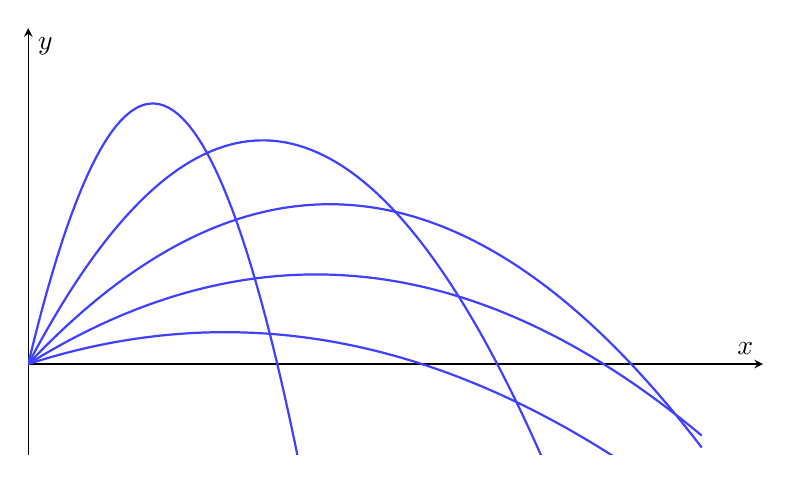
\begin{tikzpicture}
\begin{axis}[width=.90\linewidth,height=7cm,axis lines=middle,xlabel={$x$},ylabel={$y$},
 xmin=0,xmax=7.2,ymin=-1,ymax=3.7,ticks=none,clip=true]
 
 \foreach \ang in {20,35,50,65,78}{
  \addplot[Blue!75,thick,domain=0:6.6,samples=140]{x*tan(\ang)-x*x/(12*cos(\ang)^2)};
 }
\end{axis}
\end{tikzpicture}
\figcap{题图：从同一点以同一初速率、不同仰角抛出的轨迹族。}\label{ch03:ref:question-figure-2-37}
\end{minipage}\end{center}
}

\newcommand{\KQuestionBN}{%
%
\begin{center}\begin{minipage}{.96\linewidth}\centering
\begin{tikzpicture}[>=Latex]
 \coordinate (C) at (0,0);\coordinate (T) at (5,1.5);\coordinate (X) at (5.8,0);
 \draw[thick] (C)--(X) (C)--(5.6,1.68);
 \draw[kcurve,dashed,->,domain=0:5,samples=100] plot(\x,{tan(55)*\x-(5*tan(55)-1.5)*\x*\x/25});
 \draw[vector] (C)--(55:1.3) node[above left]{$v_0$};
 \draw[TextGray] (.75,0) arc[start angle=0,end angle={atan(.3)},radius=.75];
 \draw[TextGray] (1.3,0) arc[start angle=0,end angle=55,radius=1.3];
 \node at (.99,.10){$\alpha$};\node at (1.48,.75){$\beta$};
 \draw[kguide] (T)--(5,0);
 \draw[<->,TextGray] (0,-.55)--(5,-.55) node[midway,below]{$L$};
 \node[point,label=below left:$C$] at (C){};\node[point,label=above right:$T$] at (T){};
\end{tikzpicture}
\figcap{题图：坡脚 C、坡上目标 T；$\alpha$ 为坡角，$\beta$ 为发射仰角。}\label{ch03:ref:question-figure-2-39}
\end{minipage}\end{center}
}

\newcommand{\KQuestionBO}{%
%
\begin{center}\begin{minipage}{.96\linewidth}\centering
\begin{tikzpicture}[>=Latex]
 \draw[thick] (-.3,0)--(6.5,0) (5,0)--(5,2);
 \draw[kcurve,dashed,domain=0:5,samples=100] plot(\x,{2-2*(\x-5)^2/25});
 \draw[vector] (0,0)--({1.3/sqrt(1.64)},{1.04/sqrt(1.64)}) node[above left]{$v_0$};
 \draw[vector] (5,2)--(6.3,2) node[midway,above]{$v_T$};
 \draw[TextGray] (.7,0) arc[start angle=0,end angle={atan(.8)},radius=.7];
 \node at (1.02,.31){$\theta$};
 \draw[<->,TextGray] (0,-.55)--(5,-.55) node[midway,below]{$L$};
 \draw[<->,TextGray] (5.5,0)--(5.5,2) node[midway,right]{$H$};
 \node[below left] at (0,0){$A$};\node[above left] at (5,2){$T$};
\end{tikzpicture}
\figcap{题图：要求抛体在障碍顶端 T 处的速度平行于水平地面。}\label{ch03:ref:question-figure-2-40}
\end{minipage}\end{center}
}

\newcommand{\KQuestionBP}{%
%
\begin{center}\begin{minipage}{.96\linewidth}\centering
\begin{tikzpicture}[scale=.95,>=Latex]
 \pgfmathsetmacro{\thetaLaunch}{20+atan(1/(2*tan(20)))}
 \pgfmathsetmacro{\uu}{tan(\thetaLaunch)}
 \pgfmathsetmacro{\kk}{(\uu-tan(20))/4.5}
 \coordinate (A) at (0,0);\coordinate (P) at (4.5,{4.5*tan(20)});
 \coordinate (B) at (5.6,{5.6*tan(20)});\coordinate (V) at ($(P)+(-70:1.2)$);
 \draw[thick] (A)--(5.9,0) (A)--(B)--(5.6,0);
 \draw[kcurve,dashed,domain=0:4.5,samples=100] plot(\x,{\uu*\x-\kk*\x*\x});
 \draw[vector] (A)--(\thetaLaunch:1.3) node[above left]{$v_0$};
 \draw[vector] (P)--(V) node[right=3pt]{$v_P$};
 \draw pic[draw=TextGray,angle radius=4mm] {right angle=A--P--V};
 \draw[TextGray] (.7,0) arc[start angle=0,end angle=20,radius=.7];
 \draw[TextGray] (1.3,0) arc[start angle=0,end angle=\thetaLaunch,radius=1.3];
 \node at (.96,.14){$\alpha$};\node at (1.42,.9){$\theta$};
 \node[point,label=above right:$P$] at (P){};
\end{tikzpicture}
\figcap{题图：从斜面底端抛出，要求再次碰到斜面时速度垂直于斜面。}\label{ch03:ref:question-figure-2-41}
\end{minipage}\end{center}
}

\newcommand{\KQuestionBR}{%
%
\begin{center}\begin{minipage}{.98\linewidth}\centering
\begin{tikzpicture}[scale=1,>=Latex]
 \pgfmathsetmacro{\hh}{1/(1-.45^2)}\pgfmathsetmacro{\xa}{1.4-1.8/1.45}
 \draw[very thick] (-.1,3)--(2.3,3)--(2.3,2)--(4.1,2)--(4.1,1)--(5.9,1)--(5.9,0)--(7.8,0);
 \draw[kcurve,domain=0:1,samples=70] plot({\xa+(1.4-\xa)*\x},{3+\hh-\hh*\x*\x});
 \foreach \n in {0,1,2}{
  \draw[kcurve,domain=0:1,samples=90] plot({1.4+1.8*\n+1.8*\x},{3-\n+2*.45/(1-.45)*\x-(1+.45)/(1-.45)*\x*\x});
 }
 \foreach \n in {0,1,2,3}{\node[point,label=below:{$C_{\n}$}] at ({1.4+1.8*\n},{3-\n}){};}
 \draw[vector] (\xa,{3+\hh})--++(1.1,0) node[midway,above]{$v_0$};
 \node[above left] at (\xa,{3+\hh}){$A$};
 \draw[<->,TextGray] (-.45,3)--(-.45,{3+\hh}) node[midway,left]{$H$};
 \draw[<->,TextGray] (3.2,3.55)--(5,3.55) node[midway,above]{$d$};
 \draw[<->,TextGray] (7.4,0)--(7.4,1) node[midway,right]{$l$};
\end{tikzpicture}
\figcap{题图：A 在首个踏面上方 $H$；台阶宽 $d$、高 $l$，小球逐次反弹。}\label{ch03:ref:question-figure-2-43}
\end{minipage}\end{center}
}

\newcommand{\KQuestionBT}{%
\begin{center}\begin{minipage}{.97\linewidth}\centering
\begin{tikzpicture}[>=Latex,scale=.9]

\draw[thick] (-1.8,0)--(4.1,0);\draw[thick] (0,1.3) circle(1.3);
\coordinate (A) at (3.2,0);\coordinate (T) at (0,2.6);\coordinate (O) at (0,1.3);
\draw[kguide] (0,0)--(T);
\draw[kcurve,dashed,domain=0:3.2,samples=100] plot(\x,{2.6+.75*\x-(5/10.24)*\x*\x});
\pgfmathsetmacro{\launchangle}{180-atan(2.375)}
\draw[vector] (A)--++(\launchangle:1.3) node[above right]{$v_0$};
\draw[vector] (T)--++(-.8,-.6) node[above left]{$v_T$};
\draw[<->] (0,-.55)--(3.2,-.55) node[midway,below]{$d$};
\draw (O)--(-1.3,1.3) node[midway,above]{$R$};
\draw (A)++(\launchangle:.75) arc(\launchangle:180:.75);\node at (2.2,.38){$\theta$};
\node[point,label=below:$O$] at (O){};\node[point,label=above left:$T$] at (T){};
\node[point,label=below right:$A$] at (A){};

\end{tikzpicture}
\figcap{题图：A 为抛出点，T 为球顶；虚线仅示意一条可行轨迹，并非唯一轨迹。}\label{ch03:ref:question-figure-2-45}
\end{minipage}\end{center}
}


加速度的大小和方向均不变的运动称为匀加速运动。若 $t=0$ 时质点位于 $\vect r_0$、速度为 $\vect v_0$，加速度为常矢量 $\vect a$，则
\begin{equation}
 \vect v(t)=\vect v_0+\vect a t,\qquad
 \vect r(t)=\vect r_0+\vect v_0t+\frac12\vect a t^2.
\end{equation}

这两个矢量方程同时包含各坐标方向的运动规律。任选固定直角坐标系，把 $\vect r_0,\vect v_0,\vect a$ 分解到各轴，便可得到相互独立的分量方程；再把同一时刻各分量合起来，就还原出空间中的位置和速度。这种“先分解、分别研究、再合成”的方法并非抛体运动专用，而是处理一般匀加速运动的基本工具。

在地球表面附近抛出的物体，若空气阻力可忽略，运动过程中加速度恒为重力加速度 $\vect g$，方向竖直向下。这样的运动称为抛体运动。若初速度仅有竖直分量，轨迹是直线；若初速度有水平分量，轨迹是抛物线。抛体运动容易观察，它所用的分解、合成方法也可推广到一般匀加速运动。

理想模型中的“只受重力”包括两个条件：运动范围内可把 $g$ 视为常量，并且空气阻力相对重力足够小。此时水平分速度不受重力改变，竖直分速度每秒减少 $g$。物体是否正在上升、位于最高点或已经下降，只改变 $v_y$ 的符号，不改变加速度始终向下这一事实。

取抛出点为原点，$x$ 轴水平向前，$y$ 轴竖直向上。初速率为 $v_0$，与水平面夹角为 $\theta$，则
\begin{align}
v_x(t)&=v_0\cos\theta,&x(t)&=v_0\cos\theta\,t,\\
v_y(t)&=v_0\sin\theta-gt,&y(t)&=v_0\sin\theta\,t-\frac12gt^2.
\end{align}
这就是把平面曲线运动分解为水平方向的匀速运动和竖直方向的匀变速运动。由 $t=x/(v_0\cos\theta)$ 消去时间，得到轨迹方程
\begin{equation}
 \boxed{y=x\tan\theta-\frac{gx^2}{2v_0^2\cos^2\theta}}.
\end{equation}
它是开口向下的抛物线。$v_0=0$ 时为自由落体；$\theta=\pi/2$ 或 $-\pi/2$ 时为竖直上抛或竖直下抛；$\theta=0$ 时为平抛。

分量运动必须使用同一个时间变量：不能先独立算出两个方向各自经历的时间，再把它们任意拼接。轨迹方程由消去这个共同的 $t$ 得到，它回答“到达水平坐标 $x$ 时高度是多少”；分量方程则能进一步回答到达该点的时刻和速度。轨迹的对称轴、最高点和宽窄都由 $v_0$ 与 $\theta$ 决定，同一抛物线的上升段和下降段在等高处具有大小相同、竖直分量方向相反的速度。

当落点与抛出点等高且 $0<\theta<\pi/2$ 时，除去 $t=0$ 的根，由 $y(t)=0$ 得飞行时间
\begin{equation}
 T=\frac{2v_0\sin\theta}{g}.
\end{equation}
最高点满足 $v_y=0$，所以到达最高点的时间为 $T/2$，最大高度为 $v_0^2\sin^2\theta/(2g)$。水平射程为 $v_0\cos\theta\,T$。这些结果都依赖“始末等高”；从高台落地或落在斜面上时，不能未经修改直接使用。

在任意高度相同的上升点和下降点，机械条件相同而时刻关于最高点对称。水平分速度相同，竖直分速度大小相同、方向相反，因而总速率相同。若题目给出落地速度方向、飞行时间或最高点条件，优先利用这些对称与分量性质往往比从完整二次方程重新求解更直接。

固定初速率、改变抛射角时，同一目标点可能对应两个角度，也可能只有一个临界角或完全不可达。把 $u=\tan\theta$ 代入轨迹方程后，目标条件成为关于 $u$ 的二次方程；判别式大于零对应两条轨迹，等于零对应包络线上的唯一轨迹，小于零则不可达。图~\ref{ch03:fig:k04-ex-2-37}的可达区域正是把这一判别条件对所有目标点统一表达出来。

障碍问题不仅要让轨迹到达目标，还要保证到达前不穿过障碍。对有体积的球面、墙面或台阶，应比较整段轨迹与边界，而不是只让终点坐标相等。
极限轨迹可能在目标之前与障碍相切，切点不一定是目标点。例~\ref{ch03:ex:k04-2-45}中，下降时命中球顶也满足题意；
不能把“球顶”自动当作“抛物线顶点”。还需区分允许擦边的临界轨迹与要求完全不提前接触的实际轨迹。

最终还应检查时间为正、根号内非负、发射角处在题设范围，并把所得轨迹代回边界条件。任何一个代数根若对应反向发射、碰撞发生在抛出前或提前穿过障碍，都不是物理解。

\begin{origexamplebox}{网球发球的最低击球高度}\label{ch03:ex:k04-2-32}
网球场总长为 $2L$，球网高 $h$，发球区远端距球网为 $l$。把发球简化为从高度 $H$ 处以速率 $v_0$ 水平抛出。证明：要使球越过球网并落入规定区域，$H$ 必须大于某个值 $H_0$，并求 $H_0$。
\par 题图见图~\ref{ch03:ref:question-figure-2-32}。
\KQuestionBG
\end{origexamplebox}
\Needspace{6\baselineskip}\begin{xesolution}
以下推导所用的解图为图~\ref{ch03:fig:k04-ex-2-32}。

令 $k=g/(2v_0^2)$，则球的高度为 $y=H-kx^2$。越过 $x=L$ 处球网要求
\[
 k<\frac{H-h}{L^2};
\]
\TennisServeDiagram

在发球区远端 $x=L+l$ 之前落地要求
\[
 \sqrt{\frac Hk}\le L+l,\qquad k\ge\frac{H}{(L+l)^2}.
\]
两条件能由同一个 $k$ 满足，必须有
\[
 \frac{H}{(L+l)^2}<\frac{H-h}{L^2}.
\]
整理得
\[
 \boxed{H>H_0=\frac{h(L+l)^2}{l(2L+l)}}.
\]
等号对应擦网的临界情形，故合法发球需取严格大于。落点在球网之后的条件可与上述不等式同时满足。
\end{xesolution}


\begin{origexamplebox}{落地速度方向}\label{ch03:ex:k04-2-33}
石块从 $20\,\mathrm m$ 高处水平抛出，落地速度与水平面成 $45^\circ$。求抛出速度。
\par 题图见图~\ref{ch03:ref:question-figure-2-33}。
\KQuestionBH
\end{origexamplebox}
\Needspace{6\baselineskip}\begin{xesolution}
以下推导所用的解图为图~\ref{ch03:fig:k04-ex-2-33}。

落地时竖直分速度大小 $v_y=\sqrt{2gh}$，水平分速度始终为 $v_0$。速度与水平面成 $45^\circ$，故 $v_0=v_y$：
\[
 \boxed{v_0=\sqrt{2gh}}.
\]
\HorizontalThrowImpactDiagram

取 $g=10\,\mathrm{m/s^2}$、$h=20\,\mathrm m$，得 $\boxed{v_0=20\,\mathrm{m/s}}$。
\end{xesolution}

\begin{origexamplebox}{斜抛射程}\label{ch03:ex:k04-2-34}
证明：以初速率 $v_0$、仰角 $\theta$ 抛出的物体，回到抛出点同一高度时的射程为
\[
 S=\frac{v_0^2}{g}\sin2\theta,
\]
并证明同一初速率下 $45^\circ$ 斜抛射程最大。
\par 题图见图~\ref{ch03:ref:question-figure-2-34}。
\KQuestionBI
\end{origexamplebox}
\Needspace{6\baselineskip}\begin{xesolution}
以下推导所用的解图为图~\ref{ch03:fig:k04-ex-2-34}。

除 $t=0$ 外，由 $y(t)=0$ 得飞行时间 $T=2v_0\sin\theta/g$，于是
\[
 S=v_0\cos\theta\,T
 =\frac{2v_0^2\sin\theta\cos\theta}{g}
 =\boxed{\frac{v_0^2}{g}\sin2\theta}.
\]
\ProjectileRangeDiagram

因 $\sin2\theta\le1$，最大值在 $2\theta=90^\circ$ 即 $\boxed{\theta=45^\circ}$ 处取得，$S_{\max}=v_0^2/g$。
\end{xesolution}


\begin{origexamplebox}{互余抛射角}\label{ch03:ex:k04-2-35}
同一初速率 $v_0$ 下，仰角 $\theta_1$ 的射程为 $S$。证明仰角 $\theta_2=\pi/2-\theta_1$ 的射程也为 $S$，并求两次飞行时间乘积 $t_1t_2$。
\par 题图见图~\ref{ch03:ref:question-figure-2-35}。
\KQuestionBJ
\end{origexamplebox}
\Needspace{6\baselineskip}\begin{xesolution}
以下推导所用的解图为图~\ref{ch03:fig:k04-ex-2-35}。

$\sin2\theta_2=\sin(\pi-2\theta_1)=\sin2\theta_1$，故射程相同。又
\[
t_1=\frac{2v_0\sin\theta_1}{g},\qquad
t_2=\frac{2v_0\cos\theta_1}{g},
\]
\ComplementaryProjectileDiagram

所以
\[
 t_1t_2=\frac{2v_0^2\sin2\theta_1}{g^2}
 =\boxed{\frac{2S}{g}}.
\]
\end{xesolution}

\begin{origexamplebox}{越过障碍物的最小速度}\label{ch03:ex:k04-2-36}
从 $A$ 点抛出的物体要越过水平距离为 $L$、高度为 $H$ 的障碍物，求所需的最小初速率。
\par 题图见图~\ref{ch03:ref:question-figure-2-36}。
\KQuestionBK
\end{origexamplebox}
\Needspace{6\baselineskip}\begin{xesolution}
以下推导所用的解图为图~\ref{ch03:fig:k04-ex-2-36}。

令 $u=\tan\theta$。轨迹通过临界点 $(L,H)$ 时
\[
H=Lu-\frac{gL^2}{2v_0^2}(1+u^2),
\quad
v_0^2=\frac{gL^2(1+u^2)}{2(Lu-H)}.
\]
\ObstacleClearanceDiagram

由于速度平方必须为正，先限定 $Lu-H>0$，即 $u>H/L$。
对 $u$ 求导，保留决定符号的部分：
\[
 \frac{\dd v_0^2}{\dd u}
 =\frac{gL^2}{2}\,
 \frac{2u(Lu-H)-L(1+u^2)}{(Lu-H)^2}
 =\frac{gL^2}{2}\frac{Lu^2-2Hu-L}{(Lu-H)^2}.
\]
分子为零有两根。负号根小于 $H/L$，不满足可达条件；取正号根得
\[
u=\frac{H+\sqrt{H^2+L^2}}{L}.
\]
代回可得
\[
 \boxed{v_{\min}=\sqrt{g\bigl(\sqrt{L^2+H^2}+H\bigr)}}.
\]
在 $u\to(H/L)^+$ 与 $u\to+\infty$ 两端，$v_0^2$ 均趋于无穷，且允许范围内只有这一个驻点，因此它确为全局极小值。
相应最优角满足 $\tan\theta=(H+\sqrt{H^2+L^2})/L$。
式中 $g$ 乘长度后开方，量纲为速度；$H=0$ 时恢复 $\theta=45^\circ$ 和 $v_0=\sqrt{gL}$。
图中所画的是经过顶端的边界轨迹。若“越过”要求不碰顶端，则速度必须略大于该界限，严格说该值为下确界。
\end{xesolution}

\begin{origexamplebox}{固定速率的可达区域}\label{ch03:ex:k04-2-37}
质点从给定点 $A$ 以固定速率 $v_0$、不同方向抛出。求所有可能到达区域与不可到达区域的分界线。
\par 题图见图~\ref{ch03:ref:question-figure-2-37}。
\KQuestionBL
\end{origexamplebox}
\Needspace{6\baselineskip}\begin{xesolution}
以下推导所用的解图为图~\ref{ch03:fig:k04-ex-2-37}。

把轨迹写成 $u=\tan\theta$ 的二次式：
\[
y=xu-\frac{gx^2}{2v_0^2}(1+u^2).
\]
\ProjectileReachabilityDiagram

先取 $x>0$。记 $K=gx^2/(2v_0^2)>0$，按 $u$ 配方：
\[
 y=-K\left(u-\frac{v_0^2}{gx}\right)^2
    +\frac{v_0^2}{2g}-\frac{gx^2}{2v_0^2}.
\]
平方项不能为负，所以在给定横坐标处，任何抛射角能到达的高度都不超过最后两项。
当 $u=v_0^2/(gx)$ 时平方项为零，这个最高位置确实能到达。因此包络线为
\[
 \boxed{y=\frac{v_0^2}{2g}-\frac{gx^2}{2v_0^2}}.
\]
在图示 $x>0$ 半平面内，包络线以下有两个关于 $u$ 的实根，边界上两根重合，边界上方无实根。
各实际轨迹只能与包络线相切，不能穿到它的上方。
若题意允许向左右各方向抛射，则 $x<0$ 的情形由左右对称得到，分界线方程不变。
$x=0$ 必须单独处理：竖直上抛的最高高度是 $v_0^2/(2g)$，正好是包络线顶点，不能在此处使用含 $1/x$ 的最优角公式。
这里没有引入地面等额外障碍；若存在地面，还须把可达集合与允许运动空间相交。
\end{xesolution}


\begin{origexamplebox}{铅球的最佳出手角}\label{ch03:ex:k04-2-38}
运动员能使铅球以最大速率 $v_0$ 从离地 $H$ 处出手。求最大水平射程对应的出手角；当 $v_0=12.37\,\mathrm{m/s}$、$H=1.5\,\mathrm m$ 时，求角度与成绩。

\begin{qualityfigure}
\begin{tikzpicture}[>=Latex,font=\small]
\draw[thick] (-.5,-1)--(6,-1) node[right]{地面};
\coordinate (O) at (0,1);\coordinate (P) at (5,-1);
\fill (O) circle(2pt) node[left]{$O$};\fill (P) circle(2pt) node[below]{$P$};
\draw[<->] (-.4,-1)--(-.4,1) node[midway,left]{$H$};
\draw[dashed] (O)--(5,1);\draw[->,DeepBlue,thick] (O)--(1.3,2) node[right]{$v_0$};\draw (1,1) arc(0:37.57:1) node[midway,right]{$\theta$};\draw[DeepBlue,domain=0:5,samples=60] plot(\x,{1+.8*\x-.24*\x*\x});
\end{tikzpicture}
\figcap{从高于地面的出手点射向落点}\label{mech:03:38:q}
\end{qualityfigure}
\end{origexamplebox}
\Needspace{6\baselineskip}\begin{xesolution}
\begin{qualityfigure}
\begin{tikzpicture}[>=Latex,font=\small]
\draw[thick] (-.5,-1)--(6,-1) node[right]{地面};
\coordinate (O) at (0,1);\coordinate (P) at (5,-1);
\fill (O) circle(2pt) node[left]{$O$};\fill (P) circle(2pt) node[below]{$P$};
\draw[<->] (-.4,-1)--(-.4,1) node[midway,left]{$H$};
\draw[dashed] (O)--(5,1);\draw[->,DeepBlue,thick] (O)--(1.3,2) node[right]{$v_0$};\draw (1,1) arc(0:37.57:1) node[midway,right]{$\theta$};\draw[DeepBlue,domain=0:5,samples=60] plot(\x,{1+.8*\x-.24*\x*\x});\draw[<->,Gold] (0,-1.6)--(5,-1.6) node[midway,below]{$R$};\draw[->] (0,1)--(0,2.7) node[above]{$y$};\node[above right] at (5,-1){$(R,-H)$};
\end{tikzpicture}
\figcap{从高于地面的出手点射向落点（解答用辅助图）}\label{mech:03:38:a}
\end{qualityfigure}
图~\ref{mech:03:38:a}中，以出手点 $O$ 为坐标原点，地面是 $y=-H$，落点 $P$ 的坐标为 $(R,-H)$。把这一边界代入轨迹方程，才可对出手角优化。

落地时间为
\[
T=\frac{v_0\sin\theta+\sqrt{v_0^2\sin^2\theta+2gH}}{g},
\]
这里取了落地时间的正根，负根没有飞行意义。射程为 $R=v_0\cos\theta\,T$。
直接对含根式的表达式求导较繁琐，可以把“给定 $R$ 是否能到达地面”写成同一个问题。
以出手点为原点，落点为 $(R,-H)$，令 $u=\tan\theta$，则
\[
 -H=Ru-\frac{gR^2}{2v_0^2}(1+u^2)
 =-\frac{gR^2}{2v_0^2}
   \left(u-\frac{v_0^2}{gR}\right)^2
   +\frac{v_0^2}{2g}-\frac{gR^2}{2v_0^2}.
\]
存在实数抛射角的条件为
\[
 -H\le\frac{v_0^2}{2g}-\frac{gR^2}{2v_0^2}
 \quad\Longleftrightarrow\quad
 g^2R^2\le v_0^4+2gHv_0^2.
\]
最大射程对应等号；此时平方项必须为零，于是
$u_{\rm opt}=v_0^2/(gR_{\max})$。分别求出 $R_{\max}$ 和 $u_{\rm opt}$，得到
\[
 \boxed{\tan\theta_{\rm opt}=\frac{v_0}{\sqrt{v_0^2+2gH}}},
 \qquad
 \boxed{R_{\max}=\frac{v_0}{g}\sqrt{v_0^2+2gH}}.
\]
取 $g=9.8\,\mathrm{m/s^2}$，得 $\theta_{\rm opt}\approx42.5^\circ$，$R_{\max}\approx17.1\,\mathrm m$。出手点高于地面，所以最佳角小于 $45^\circ$。
\end{xesolution}

\begin{origexamplebox}{山坡靶的炮口初速}\label{ch03:ex:k04-2-39}
炮位看靶子的仰角为 $\alpha$，炮与靶的水平距离为 $L$，炮身仰角为 $\beta$。求击中目标所需的初速率。
\par 题图见图~\ref{ch03:ref:question-figure-2-39}。
\KQuestionBN
\end{origexamplebox}
\Needspace{6\baselineskip}\begin{xesolution}
以下推导所用的解图为图~\ref{ch03:fig:k04-ex-2-39}。

目标坐标为 $(L,L\tan\alpha)$。代入轨迹方程：
\[
L\tan\alpha=L\tan\beta-
\frac{gL^2}{2v_0^2\cos^2\beta}.
\]
\HillsideTargetDiagram

所以
\[
 \boxed{v_0=\sqrt{\frac{gL}{2\cos^2\beta(\tan\beta-\tan\alpha)}}},
\]
并要求 $\beta>\alpha$，否则根号内不为正，理想抛体轨迹不能击中该点。
\end{xesolution}

\ProjectileVectorsDiagram

除逐分量列方程外，抛体运动还可作矢量合成：
\begin{equation}
 \vect v(t)=\vect v_0+\vect g t,
 \qquad
 \vect r(t)=\vect v_0t+\frac12\vect g t^2.
\end{equation}
图~\ref{ch03:fig:k04-2-12}中，$\vect v_0$ 与 $\vect v_0t$ 平行，但两个实线三角形一般并不相似：重力项的相对长度差一个因子 $2$。
图示时刻物体正在下降，因此 $\vect v$ 向右下；但它仍高于抛出点，因此 $\vect r$ 向右上。
从右图 $\vect r$ 的终点再接一段 $\frac12\vect g t^2$，得到的新合矢量为
\[
 \vect r+\frac12\vect g t^2
 =\vect v_0t+\vect g t^2=t(\vect v_0+\vect gt)=t\vect v.
\]
这个补上虚线的外侧三角形，其三条边才分别是速度三角形三边的 $t$ 倍。
几何方向相同不代表速度与位移量纲相同；乘上同一时间后才可逐边比较。

几何法的关键是保留矢量方向。$\vect g t$ 必须从 $\vect v_0$ 的终点接出，才能得到时刻 $t$ 的速度；$\frac12\vect g t^2$ 同理从 $\vect v_0t$ 的终点接出，得到相对抛出点的位移。若只把三个矢量的大小写成普通加法，便会丢失上升与下降、锐角与钝角等方向信息。遇到障碍、斜面或固定瞄准线时，矢量图常能直接揭示相似三角形和投影关系，减少繁琐的坐标消元。

\begin{origexamplebox}{在障碍物顶端水平飞过}\label{ch03:ex:k04-2-40}
水平地面上距 $A$ 点 $L$ 处有高为 $H$ 的障碍物。从 $A$ 抛出的物体恰在通过障碍物上端时速度水平，求抛射仰角 $\theta$ 和初速率 $v_0$。
\par 题图见图~\ref{ch03:ref:question-figure-2-40}。
\KQuestionBO
\end{origexamplebox}
\Needspace{6\baselineskip}\begin{xesolution}
以下推导所用的解图为图~\ref{ch03:fig:k04-ex-2-40}。

障碍物顶端即轨迹最高点。最高点条件给出
\[
H=\frac{v_0^2\sin^2\theta}{2g},\qquad
L=\frac{v_0^2\sin\theta\cos\theta}{g}.
\]
\HorizontalAtObstacleDiagram

相除得
\[
 \boxed{\tan\theta=\frac{2H}{L}},
\]
再代回任一式，得
\[
 \boxed{v_0=\sqrt{\frac{g(L^2+4H^2)}{2H}}}.
\]
\end{xesolution}

\begin{origexamplebox}{垂直撞上斜面}\label{ch03:ex:k04-2-41}
从倾角为 $\alpha$ 的斜面底部斜向上抛出物体。仰角 $\theta$ 为何值时，物体击中斜面时的速度恰与斜面垂直？
\par 题图见图~\ref{ch03:ref:question-figure-2-41}。
\KQuestionBP
\end{origexamplebox}
\Needspace{6\baselineskip}\begin{xesolution}
以下推导所用的解图为图~\ref{ch03:fig:k04-ex-2-41}。

以抛出点为原点，水平向右为 $x$ 轴、竖直向上为 $y$ 轴。
图示构型取 $0<\alpha<\pi/2$、$\alpha<\theta<\pi/2$，即物体先进入斜面上方的空间。
抛体的位置为
\[
 x=v_0\cos\theta\,t,\qquad y=v_0\sin\theta\,t-\frac12gt^2.
\]
\InclinedPlaneNormalImpactDiagram

再次击中斜面时满足 $y=x\tan\alpha$，代入后整理为
\[
 t\left[v_0(\sin\theta-\cos\theta\tan\alpha)-\frac12gt\right]=0.
\]
其中 $t=0$ 只是抛出瞬间，不是所求的再次碰撞。利用
$\sin\theta-\cos\theta\tan\alpha=\sin(\theta-\alpha)/\cos\alpha$，
得到正的飞行时间
\[
t=\frac{2v_0\sin(\theta-\alpha)}{g\cos\alpha}.
\]
斜面切向单位矢量为 $(\cos\alpha,\sin\alpha)$。速度垂直斜面要求切向分量为零：
\[
v_0\cos(\theta-\alpha)-gt\sin\alpha=0.
\]
代入 $t$ 后
\[
\cot(\theta-\alpha)=2\tan\alpha,
\]
因此
\[
 \boxed{\theta=\alpha+\arctan\!\left(\frac{1}{2\tan\alpha}\right)}.
\]
这里反正切取 $(0,\pi/2)$ 内的值。由于
$1/(2\tan\alpha)<\cot\alpha$，所得 $\theta-\alpha<\pi/2-\alpha$，
确实满足 $\alpha<\theta<\pi/2$。此时法向速度指向斜面，表示撞入而不是离开斜面；
飞行时间中的 $v_0/g$ 具有时间量纲，角度关系与初速率无关。
\end{xesolution}

因为抛体运动非常普遍，上述标准公式并不能自动替代建模。处理新题时应先确定坐标系、初始位置、落点或碰撞点的几何条件，再把同一时刻的水平和竖直方程联立。若题目含台阶、反弹或球面障碍，还要逐段检查碰撞后的速度规则以及整段轨迹是否提前与障碍相交，不能只验证终点坐标。


\begin{origexamplebox}{轰炸机瞄准镜}\label{ch03:ex:k04-2-42}
轰炸机在离地高度 $H$ 处以速率 $v$ 水平匀速飞行。设计瞄准镜，使飞行员在目标位于十字线正中时投弹即可命中。求瞄准镜轴线与竖直线的夹角。

\begin{qualityfigure}
\begin{tikzpicture}[>=Latex,font=\small]
\draw[thick] (-.5,-1)--(6,-1) node[right]{地面};
\coordinate (O) at (0,1);\coordinate (P) at (5,-1);
\fill (O) circle(2pt) node[left]{$O$};\fill (P) circle(2pt) node[below]{$P$};
\draw[<->] (-.4,-1)--(-.4,1) node[midway,left]{$H$};
\draw[dashed] (O)--(5,1);\draw[->,DeepBlue,thick] (O)--(1.7,1) node[above]{$v$};\draw[dashed] (O)--(P);\draw[dashed] (O)--(0,-1);\draw (0,.3) arc(-90:-21.8:.7) node[midway,below right]{$\phi$};
\end{tikzpicture}
\figcap{投弹点、竖直线与目标视线}\label{mech:03:42:q}
\end{qualityfigure}
\end{origexamplebox}
\Needspace{6\baselineskip}\begin{xesolution}
\begin{qualityfigure}
\begin{tikzpicture}[>=Latex,font=\small]
\draw[thick] (-.5,-1)--(6,-1) node[right]{地面};
\coordinate (O) at (0,1);\coordinate (P) at (5,-1);
\fill (O) circle(2pt) node[left]{$O$};\fill (P) circle(2pt) node[below]{$P$};
\draw[<->] (-.4,-1)--(-.4,1) node[midway,left]{$H$};
\draw[dashed] (O)--(5,1);\draw[->,DeepBlue,thick] (O)--(1.7,1) node[above]{$v$};\draw[dashed] (O)--(P);\draw[dashed] (O)--(0,-1);\draw (0,.3) arc(-90:-21.8:.7) node[midway,below right]{$\phi$};\draw[Gold,thick,domain=0:5,samples=50] plot(\x,{1-2*\x*\x/25});\draw[<->] (0,-1.6)--(5,-1.6) node[midway,below]{$D=vt$};
\end{tikzpicture}
\figcap{投弹点、竖直线与目标视线（解答用辅助图）}\label{mech:03:42:a}
\end{qualityfigure}
图~\ref{mech:03:42:a}中，$OP$ 是投弹瞬间的瞄准线，$H$ 是竖直落差，$D$ 是水平超前距离；夹角 $\phi$ 从竖直线量起，因此用 $\tan\phi=D/H$。

炸弹下落时间 $t=\sqrt{2H/g}$，在此期间水平前进
\[
D=vt=v\sqrt{\frac{2H}{g}}.
\]
投弹瞬间目标应位于飞机前下方，视线与竖直方向夹角 $\phi$ 满足
\[
 \boxed{\tan\phi=\frac DH=v\sqrt{\frac{2}{gH}}}.
\]
因此瞄准镜应沿此前下方视线设置；忽略空气阻力时炸弹保留飞机的水平速度。
\end{xesolution}

\begin{origexamplebox}{台阶上的全同反弹}\label{ch03:ex:k04-2-43}
每级台阶长 $d$、高 $l$。球从 $A$ 点以水平速度 $v_0$ 抛出；碰撞后水平分速度不变，竖直分速度反向并变为碰撞前的 $e$ 倍，$e<1$。若每次碰撞前与台阶的相对速度相同，轨迹形成全同的往复过程，求 $v_0$ 和每次反弹后的上升高度。
\par 题图见图~\ref{ch03:ref:question-figure-2-43}。
\KQuestionBR
\end{origexamplebox}
\Needspace{6\baselineskip}\begin{xesolution}
以下推导所用的解图为图~\ref{ch03:fig:k04-ex-2-43}。

设每次碰撞前竖直分速度大小为 $V$，则碰撞后向上为 $eV$。下一碰撞点比前一点低 $l$，由竖直运动的速度—位移关系
\[
V^2=e^2V^2+2gl,
\quad
V=\sqrt{\frac{2gl}{1-e^2}}.
\]
\StairBounceDiagram

相邻碰撞间的时间等于竖直速度从 $+eV$ 变到 $-V$ 所需时间：
\[
T=\frac{(1+e)V}{g}.
\]
水平位移为 $d=v_0T$，故
\[
 \boxed{v_0=d\sqrt{\frac{g(1-e)}{2l(1+e)}}}.
\]
每次反弹后的上升高度为
\[
 \boxed{h_b=\frac{e^2V^2}{2g}=\frac{e^2l}{1-e^2}}.
\]
若题图另以 $H$ 表示首次下落高度，全同条件还要求 $H=l/(1-e^2)$，于是 $h_b=e^2H$。
\end{xesolution}

\begin{origexamplebox}{反弹轨迹的面积和}\label{ch03:ex:k04-2-44}
小球从距水平地面 $h$ 高处，以水平速度 $\sqrt{2gh}$ 抛出。每次落地反弹时水平速度不变，竖直速度反向且按固定比率 $e$ 减小，其中 $0<e<1$。若从第一次反弹开始，各段轨迹与地面所围面积之和为 $\frac{8}{21}h^2$，求 $e$。提示：一次从地面出发又落回地面的斜抛轨迹所围面积，等于其最大高度与射程乘积的 $2/3$。

\begin{qualityfigure}
\begin{tikzpicture}[>=Latex,font=\small]
\begin{scope}[y=2cm]\draw[thick](-.5,0)--(6.4,0);\fill(0,1)circle(2pt);\draw[<->](-.4,0)--(-.4,1)node[midway,left]{$h$};
\draw[->,DeepBlue](0,1)--(1.2,1)node[right]{$\sqrt{2gh}$};
\draw[DeepBlue,domain=0:2,samples=40]plot(\x,{1-\x*\x/4});
\draw[DeepBlue,domain=2:4.4,samples=40]plot(\x,{.25*(\x-2)*(4.4-\x)});
\draw[DeepBlue,domain=4.4:5.84,samples=40]plot(\x,{.25*(\x-4.4)*(5.84-\x)});\end{scope}
\end{tikzpicture}
\figcap{反弹后的抛物线弓形面积}\label{mech:03:44:q}
\end{qualityfigure}
\end{origexamplebox}
\Needspace{6\baselineskip}\begin{xesolution}
\begin{qualityfigure}
\begin{tikzpicture}[>=Latex,font=\small]
\begin{scope}[y=2cm]\fill[PaleBlue,domain=2:4.4,samples=40](2,0)--plot(\x,{.25*(\x-2)*(4.4-\x)})--cycle;\draw[thick](-.5,0)--(6.4,0);\fill(0,1)circle(2pt);\draw[<->](-.4,0)--(-.4,1)node[midway,left]{$h$};
\draw[->,DeepBlue](0,1)--(1.2,1)node[right]{$\sqrt{2gh}$};
\draw[DeepBlue,domain=0:2,samples=40]plot(\x,{1-\x*\x/4});
\draw[DeepBlue,domain=2:4.4,samples=40]plot(\x,{.25*(\x-2)*(4.4-\x)});
\draw[DeepBlue,domain=4.4:5.84,samples=40]plot(\x,{.25*(\x-4.4)*(5.84-\x)});\draw[<->,Gold](2,-.3)--(4.4,-.3)node[midway,below]{$S_n$};\draw[<->,Gold](3.2,0)--(3.2,.36)node[midway,right]{$H_n$};\node at(3.2,.85){$A_n=\frac23H_nS_n$};\end{scope}
\end{tikzpicture}
\figcap{反弹后的抛物线弓形面积（解答用辅助图）}\label{mech:03:44:a}
\end{qualityfigure}
图~\ref{mech:03:44:a}中，阴影从某次反弹点起、到下一次落地点止，对应高度 $H_n$ 与射程 $S_n$；题目从第一次反弹开始计面积，故级数下标从 $n=1$ 起。

第一次落地前竖直速度大小为 $\sqrt{2gh}$。第 $n$ 次反弹后的竖直初速度为 $e^n\sqrt{2gh}$，故最大高度 $H_n=e^{2n}h$；水平速度为 $\sqrt{2gh}$，飞行时间 $2e^n\sqrt{2h/g}$，射程 $S_n=4e^nh$。于是第 $n$ 个面积
\[
A_n=\frac23H_nS_n=\frac83h^2e^{3n}.
\]
从 $n=1$ 起求和：
\[
\frac83h^2\frac{e^3}{1-e^3}=\frac8{21}h^2.
\]
解得 $7e^3=1-e^3$，所以
\[
 \boxed{e=\frac12}.
\]
\end{xesolution}

\begin{origexamplebox}{击中球顶的速度界限}\label{ch03:ex:k04-2-45}
地面上放有半径为 $R$ 的球体。从地面斜向上抛出一个质点，要求击中球顶，且在此之前不碰球体。
求所需初速率的下界及相应临界抛射角、抛出点到球底的距离，并判断这个下界能否取到。
同时给出允许“提前与球面相切但不穿入”时的临界结果。
\par 题图见图~\ref{ch03:ref:question-figure-2-45}。
\KQuestionBT
\end{origexamplebox}
\Needspace{6\baselineskip}\begin{xesolution}
以下推导所用的解图为图~\ref{ch03:fig:k04-ex-2-45}。

\textbf{先判断命中时的速度方向。}
物体不可能上升着从球体内部穿到球顶；但既可以在球顶水平掠过，也可以在下降时命中。
因此不能预先令球顶的竖直速度为零。下面把这两类运动统一处理。
\SphereClearanceDiagram
图中 $T$ 是球顶；左图临界轨迹在到达 $T$ 之前还与球面在 $P$ 点相切，右图则从球面上方经过后在下降阶段到达 $T$。
两个点的作用不同：$T$ 决定命中，$P$ 决定是否提前碰球。

\textbf{把全部候选轨迹写成两个参数。}
以球底为水平坐标原点，以地面为 $y=0$，抛出点在 $x=-d$。
设水平分速度为 $u>0$，到达 $T=(0,2R)$ 时的竖直分速度为 $w\le0$。
记无量纲量
\[
 s=-\frac{x}{R},\qquad q=-\frac wu\ge0,\qquad
 k=\frac{gR}{2u^2}>0.
\]
以球顶为已知点写轨迹，得到
\[
 y=2R+\frac wu x-\frac{g}{2u^2}x^2,
 \qquad \boxed{\frac{y}{R}=2+qs-ks^2}.
\]
其中 $s>0$ 表示位于球顶左侧。$q=0$ 才是球顶速度水平的特殊情况。
从抛出点到球顶上升的净高度为 $2R$。由竖直运动公式
$v_{y0}^2-w^2=4gR$，可得
\[
 \frac{v_0^2}{gR}
 =4+\frac{u^2+w^2}{gR}
 =\boxed{4+\frac{1+q^2}{2k}}.
\]
这一式同时检查了机械能：初动能减去到球顶的动能恰为 $2mgR$。

\textbf{检查到顶之前的整段球面。}
在左半球的水平投影 $0<s\le1$ 内，球体上边界为
\[
 \frac{y_s}{R}=1+\sqrt{1-s^2}.
\]
所以不穿入球体要求
\[
 2+qs-ks^2\ge1+\sqrt{1-s^2},
 \quad\text{即}\quad
 q\ge h_k(s):=ks-\frac{1-\sqrt{1-s^2}}{s}.
\]
严格“不提前接触”时，不等式在 $0<s\le1$ 必须严格成立。
在球体投影以外没有球面障碍；轨迹与地面的左交点就是抛出点。
给定 $k$ 后，速度平方随 $q\ge0$ 增加，因此应先找使整段不等式成立的最小 $q$。

若 $k\le1/2$，由于
\[
 1-\sqrt{1-s^2}=\frac{s^2}{1+\sqrt{1-s^2}}\ge\frac{s^2}{2}\ge ks^2,
\]
取 $q=0$ 已足够使轨迹位于球面上方，且
\[
 \frac{v_0^2}{gR}=4+\frac1{2k}\ge5.
\]
这给出“在球顶速度水平”一类轨迹的下界 $\sqrt{5gR}$，但它不一定是所有轨迹的下界。

若 $k>1/2$，函数 $h_k$ 在球顶附近先增加，随后下降，最大值出现在一个内部点。
为求这个点，令 $c=\sqrt{1-s^2}$。对 $s$ 求导，得到
\[
 h_k'(s)=k-\frac1{c(1+c)}.
\]
当 $s$ 从 $0$ 增加到 $1$，$c$ 从 $1$ 减少到 $0$，故第二项从 $1/2$ 单调增至无穷。
因此恰有一个最大值点，满足
\[
 k=\frac1{c(1+c)},\qquad s=\sqrt{1-c^2},\qquad 0<c<1.
\]
在该点取 $q=h_k(s)$，化简为
\[
 q=\frac{s(1-c)}{c(1+c)}.
\]
这两个等式正是提前切点 $P$ 的位置相同、斜率相同条件；并非只在球顶作局部比较。

\textbf{求所有临界轨迹中的最小速度。}
将上述 $k,q$ 代入速度式，注意 $s^2=1-c^2$：
\begin{align*}
 \frac{1+q^2}{2k}
 &=\frac{c^2(1+c)+(1-c)^3}{2c}\\
 &=2c-\frac32+\frac1{2c}.
\end{align*}
于是
\[
 \frac{v_0^2}{gR}
 =\frac52+2c+\frac1{2c}\ge\frac52+2=\frac92,
\]
其中用了 $2c>0$ 与 $(2c)^{-1}>0$ 的和不小于 $2$。
等号在 $c=1/2$ 取得，故
\[
 k_*=\frac43,\quad q_*=\frac1{\sqrt3},\quad
 u_*^2=\frac38gR,\quad w_*^2=\frac18gR,\quad w_*<0.
\]
初始竖直分速度满足 $v_{y0,*}^2=w_*^2+4gR=33gR/8$。
由 $y(-d)=0$，取正的距离根：
\[
 \frac{d}{R}=\frac{q+\sqrt{q^2+8k}}{2k}.
\]
所以临界结果为
\[
 \boxed{v_*=\frac3{\sqrt2}\sqrt{gR}},\qquad
 \boxed{\tan\theta_*=\sqrt{11}},\qquad
 \boxed{d_*=\frac{\sqrt3+3\sqrt{11}}8R}.
\]
切点位于 $x_P=-\sqrt3R/2$、$y_P=3R/2$，早于球顶 $T$。

\textbf{区分最小值和下确界。}
上述等号轨迹先碰到 $P$，因此不满足严格的“不提前接触”。
固定 $k=4/3$，取 $q=1/\sqrt3+\varepsilon$，$\varepsilon>0$，轨迹在每个 $s>0$ 处都比临界轨迹高出 $R\varepsilon s$；
它避开提前接触，仍在 $T$ 命中。令 $\varepsilon\to0^+$，其初速率可无限趋近 $v_*$。
因此：
\[
 \boxed{\text{严格不提前接触：}\quad v_0>v_*,
 \quad \inf v_0=v_*\ \text{但不存在能取到的最小值。}}
\]
这里的不等式表示任何可行轨迹的必要速度界限，且可行速度可以从上方任意逼近此界；
不能据此认为任意抛射角都能命中。若允许提前相切但不穿入，则 $v_*$ 可以取到，临界角和距离即上式。
$\sqrt{gR}$ 具有速度量纲，$d_*\propto R$、$\theta_*$ 与尺度无关；半径缩小时速度界限按 $\sqrt R$ 减小，符合几何相似缩放。
\end{xesolution}
}

{
\graphicspath{{../../../sample/xes-original/kinematics-supplement/}{../../../sample/xes-original/kinematics-supplement/assets/}}
\section{圆周运动}
\newcommand{\CirclePositionDiagram}{%
\begin{center}\begin{tikzpicture}[scale=.9,>=Latex]
 \draw[very thick] (0,0) circle (2);
 \coordinate (O) at (0,0);\coordinate (N) at (2,0);\coordinate (P) at (52:2);
 \draw[very thick] (O)--(N) node[midway,clearlabel,below]{$R$};
 \draw[very thick] (O)--(P);
 \draw[->,TextGray] (.75,0) arc[start angle=0,end angle=52,radius=.75];
 \node[clearlabel] at (1,.43){$\theta$};
 \node[point,label={[clearlabel]below left:$O$}] at (O) {};
 \node[point,label={[clearlabel]right:$N$}] at (N) {};
 \node[point,label={[clearlabel]above right:$P$}] at (P) {};
\end{tikzpicture}\figcap{角位置 $\theta$ 由固定射线 $ON$ 转到半径 $OP$ 的有向角确定；逆时针为正。}\label{ch03:fig:k05-2-13}\end{center}}

\newcommand{\AngularSignDiagram}{%
\begin{center}\begin{tikzpicture}[scale=.75,>=Latex]
 \begin{scope}[xshift=-2.4cm]
  \draw[very thick] (0,0) circle (1.25);\draw[DeepBlue,very thick,->] (1.45,-.2) arc[start angle=-8,end angle=95,radius=1.45];
  \node[clearlabel,below] at (0,-1.65){$\omega>0$（逆时针）};
 \end{scope}
 \begin{scope}[xshift=2.4cm]
  \draw[very thick] (0,0) circle (1.25);\draw[Blue,very thick,->] (-1.45,-.2) arc[start angle=188,end angle=85,radius=1.45];
  \node[clearlabel,below] at (0,-1.65){$\omega<0$（顺时针）};
 \end{scope}
\end{tikzpicture}\figcap{角速度的符号只表示转动方向，不表示快慢。}\label{ch03:fig:k05-2-14}\end{center}}

\newcommand{\CentripetalDerivationDiagram}{%
\begin{center}\begin{minipage}{.98\linewidth}\centering
\begin{tikzpicture}[scale=1,>=Latex]
 \begin{scope}[xshift=-3.5cm]
  \draw[thick] (0,0) circle (1.7);
  \coordinate (A) at (110:1.7);\coordinate (B) at (70:1.7);
  \draw[TextGray] (0,0)--(A) (0,0)--(B);
  \draw[vector] (A)--++(20:1.2) node[pos=.85,above=3pt]{$\vect v_A$};
  \draw[vector] (B)--++(-20:1.2) node[right=3pt]{$\vect v_B$};
  \draw[TextGray] (70:.65) arc[start angle=70,end angle=110,radius=.65];
  \node at (0,1.22){$|\Delta\theta|$};
  \node[point,label=above left:$A$] at (A){};
  \node[point] at (B){};\node[above right] at ($(B)+(.12,.17)$){$B$};
  \node[below] at (0,-2){(a) 同一圆周上的两速度};
 \end{scope}
 \begin{scope}[xshift=2.4cm]
  \coordinate (S) at (0,0);\coordinate (P) at (20:2.5);\coordinate (Q) at (-20:2.5);
  \draw[vector] (S)--(P) node[midway,above left]{$\vect v_A$};
  \draw[vector] (S)--(Q) node[midway,below left]{$\vect v_B$};
  \draw[vector] (P)--(Q) node[midway,right=4pt]{$\Delta\vect v$};
  \draw[TextGray] (-20:.8) arc[start angle=-20,end angle=20,radius=.8];
  \node[right] at (.85,0){$|\Delta\theta|$};
  \node[left] at (S){$S$};\node[above] at (P){$P$};\node[below] at (Q){$Q$};
  \node[below] at (1.1,-2){(b) 平移后作矢量差};
 \end{scope}
\end{tikzpicture}
\figcap{右图保持左图两速度的方向；$\Delta\vect v$ 由旧速度终点指向新速度终点。}\label{ch03:fig:k05-2-15}
\end{minipage}\end{center}}

\newcommand{\RadialCollisionBase}[1]{%
\begin{tikzpicture}[scale=.75,>=Latex]
 \draw[very thick] (0,0) circle (2);\coordinate (P) at (0,2);\coordinate (A) at (25:2);\coordinate (B) at (0,.72);
 \node[point,label={[clearlabel]below left:$O$}] at (0,0) {};
 \node[point,label={[clearlabel]above:$P$}] at (P) {};
 \node[point,label={[clearlabel]below left:$A$}] at (A) {};
 \node[point,label={[clearlabel]right:$B$}] at (B) {};
 \draw[kguide] (0,0)--(P);
 \node[clearlabel,left,xshift=-2pt] at (0,.35){$R$};
 \draw[vector] (B)--(0,1.60) node[midway,clearlabel,right,xshift=3pt]{$#1$};
 \draw[DeepBlue,very thick,->] (4:2.25) arc[start angle=4,end angle=55,radius=2.25];
 \node[right] at (2.42,1.28){$\omega$};
\end{tikzpicture}}

\newcommand{\RadialUniformCollisionDiagram}{%
\begin{center}\RadialCollisionBase{\vect v_B}
\figcap{$B$ 以恒定速度沿射线 $OP$ 运动，故与圆周质点 $A$ 的相撞点只能是 $P$。}\label{ch03:fig:k05-ex-2-47}\end{center}}

\newcommand{\RadialAcceleratedCollisionDiagram}{%
\begin{center}\RadialCollisionBase{\vect a_B}
\figcap{$B$ 从 $O$ 由静止沿 $OP$ 匀加速；几何相撞点仍只能是 $P$，但到达时间条件改变。}\label{ch03:fig:k05-ex-2-48}\end{center}}

\newcommand{\SameCirclePursuitDiagram}{%
\begin{center}\begin{tikzpicture}[scale=.8,>=Latex]
  \draw[very thick] (0,0) circle (2.25);
  \coordinate (O) at (0,0);\coordinate (P) at (90:2.25);\coordinate (Q) at (135:2.25);
  \draw[very thick] (O)--(P);\draw[kguide] (O)--(Q);
  \draw[DeepBlue,very thick,->] (125:2.5) arc[start angle=125,end angle=175,radius=2.5]
    node[midway,clearlabel,left]{$\omega_1$};
  \draw[Blue,very thick,->] (-2.5,-.55) arc[start angle=192,end angle=230,radius=2.5]
    node[midway,clearlabel,left]{$\omega_2$};
  \draw pic[draw=TextGray,->,angle radius=8mm,"$\theta$"{clearlabel}] {angle=P--O--Q};
  \node[point] at (Q) {};\node[left] at ($(Q)+(-.7,.32)$){$Q$};
  \node[point,label={[clearlabel]above:$P$}] at (P) {};
  \node[point,label={[clearlabel]below right:$O$}] at (O) {};
\end{tikzpicture}\figcap{两质点从同一点出发沿同一圆周逆时针运动，第二次相遇位置相对 $OP$ 转过角 $\theta$。}\label{ch03:fig:k05-ex-2-49}\end{center}}

\newcommand{\ConcentricCollinearityDiagram}{%
\begin{center}\begin{tikzpicture}[scale=.8,>=Latex]
  \draw[very thick] (0,0) circle (1.35);\draw[very thick] (0,0) circle (2.35);
  \coordinate (O) at (0,0);\coordinate (A) at (28:1.35);\coordinate (B) at (28:2.35);
  \draw[kguide] (O)--(B);
  \draw[vector] (A)--++(118:1.05) node[midway,clearlabel,right]{$\vect v_A$};
  \draw[vector] (B)--++(118:.82);
  \node at (2.12,2.17){$\vect v_B$};
  \draw[TextGray] (O)--(145:1.35) node[midway,clearlabel,above=3pt]{$R_1$};
  \draw[TextGray] (O)--(225:2.35);
  \node at (-1.75,-.65){$R_2$};
  \node[point] at (O) {};\node at (.25,-.30){$O$};
  \node[point,label={[clearlabel]right:$A$}] at (A) {};
  \node[point,label={[clearlabel]below right:$B$}] at (B) {};
\end{tikzpicture}\figcap{$A,B$ 分别在半径 $R_1,R_2$ 的同心圆上；题目要求两点与圆心再次共线。}\label{ch03:fig:k05-ex-2-50}\end{center}}

\newcommand{\ProjectileCircleCollisionDiagram}{%
\begin{center}\begin{minipage}{.96\linewidth}\centering
\begin{tikzpicture}[scale=1,>=Latex]
 \draw[TextGray,dashed] (3,0) arc[start angle=0,end angle=180,x radius=3,y radius=.75];
 \draw[thick] (-3,0) arc[start angle=180,end angle=360,x radius=3,y radius=.75];
 \coordinate (O) at (0,0);\coordinate (A) at (3,0);\coordinate (S) at (0,3);
 \draw[kguide] (O)--(A) (O)--(S);
 \draw[vector] (S)--(1.25,3) node[midway,above]{$v_0$};
 \draw[kcurve,dashed,->,domain=0:3,samples=90] plot(\x,{3-\x*\x/3});
 \draw[Blue,->,thick] (3.3,0) arc[start angle=0,end angle=52,x radius=3.3,y radius=.83];
 \node[above right] at (2.6,.7){$\omega$};
 \draw[<->,TextGray] (-.45,0)--(-.45,3) node[midway,left]{$H$};
 \node[below] at (1.5,0){$R$};
 \node[point,label=below left:$O$] at (O){};
 \node[point,label=right:$A$] at (A){};
 \node[point,label=above left:{$S\;(B\text{的初始位置})$}] at (S){};
\end{tikzpicture}
\figcap{$S$ 在圆心 $O$ 正上方；抛体从 $S$ 水平出发，在圆周上与整周返回的质点相遇。}\label{ch03:fig:k05-ex-2-51}
\end{minipage}\end{center}}

\newcommand{\AccelerationVelocityAngleDiagram}{%
\begin{center}\begin{minipage}{.96\linewidth}\centering
\begin{tikzpicture}[scale=.95,>=Latex]
 \draw[thick] (0,0) circle (2.0);\coordinate (P) at (35:2);
 \coordinate (V) at ($(P)+(125:1.4)$);\coordinate (A) at ($(P)+(170:1.4)$);
 \draw[kguide] (0,0)--(P) node[pos=.4,below right]{$R$};
 \draw[vector] (P)--(V) node[above right]{$\vect v$};
 \draw[vector] (P)--(A) node[above left]{$\vect a$};
 \draw pic[draw=TextGray,angle radius=7mm] {angle=V--P--A};
 % The circumference crosses this narrow wedge. Show its label separately,
 % retaining the physical vectors and the main angle arc without a mask.
 \begin{scope}[shift={(4.7,1.3)}]
 \draw[vector] (0,0)--(125:1.6) node[above right]{$\vect v$};
 \draw[vector] (0,0)--(170:1.6) node[above left]{$\vect a$};
 \draw[TextGray] (125:.6) arc(125:170:.6);
 \node at (147.5:.95){$\theta$};
 \node[below] at (-.5,-.4){夹角放大};
 \end{scope}
 \node[point,label=below left:$O$] at (0,0){};\node[point] at (P){};
\end{tikzpicture}
\figcap{右侧单独放大速度与加速度的夹角 $\theta$；该角取值在 $0$ 与 $\pi$ 之间。}\label{ch03:fig:k05-ex-2-59}
\end{minipage}\end{center}}

\newcommand{\ConcentricSightDiagram}{%
\begin{center}\begin{minipage}{.96\linewidth}\centering
\begin{tikzpicture}[scale=.9,>=Latex]
 \pgfmathsetmacro{\ax}{1.5^2/2.8}\pgfmathsetmacro{\ay}{sqrt(1.5^2-\ax^2)}
 \coordinate (O) at (0,0);\coordinate (B) at (2.8,0);\coordinate (A) at (\ax,\ay);
 \draw[thick] (O) circle (1.5) (O) circle (2.8);
 \draw[thick] (O)--(B) (B)--(A);\draw[kguide] (O)--(A);
 \draw pic[draw=TextGray,angle radius=4mm] {right angle=O--A--B};
 \draw pic[draw=TextGray,angle radius=8mm] {angle=A--B--O};
 \node at (1.75,.27){$\theta$};
 \draw[TextGray] (O)--(145:1.5) node[midway,below left]{$R_1$};
 \draw[TextGray] (O)--(230:2.8) node[pos=.78,below right=4pt]{$R_2$};
 \node[point,label=below:$O$] at (O){};\node[point,label=right:$B$] at (B){};
 \node[point,label=above:$A$] at (A){};
\end{tikzpicture}
\figcap{$A$ 为从 $B$ 引向内圆的切点，因而 $OA\perp AB$。}\label{ch03:fig:k05-ex-2-52}
\end{minipage}\end{center}}

\newcommand{\RacetrackDiagram}{%
\begin{center}\begin{tikzpicture}[scale=.72,>=Latex]
 \draw[very thick] (-2.4,-2.4)--(-2.4,0) arc[start angle=180,end angle=0,radius=2.4]--(2.4,-2.4);
 \draw[very thick] (-1.4,-2.4)--(-1.4,0) arc[start angle=180,end angle=0,radius=1.4]--(1.4,-2.4);
 \draw[->,DeepBlue,very thick] (-1.4,-1.9)--(-1.4,-.85);
 \draw[->,Blue,very thick] (-2.4,-1.9)--(-2.4,-.85);
 \draw[<->,TextGray] (0,0)--(0,1.4) node[midway,clearlabel,right]{$R_1$};
 \draw[<->,TextGray] (0,0)--(135:2.4) node[pos=.85,clearlabel,above right=3pt]{$R_2$};
 \node[clearlabel,below] at (0,-2.75){内、外路线均为半圆弯道};
\end{tikzpicture}\figcap{解图：外道允许更高速度，但半圆弧也更长。}\label{ch03:fig:k05-ex-2-57}\end{center}}

\newcommand{\KQuestionBV}{%
%
\begin{center}\RadialCollisionBase{\vect v_B}
\figcap{题图：A 沿半径为 $R$ 的圆周运动，B 沿 OP 匀速运动。}\label{ch03:ref:question-figure-2-47}\end{center}
}

\newcommand{\KQuestionBW}{%
%
\begin{center}\RadialCollisionBase{\vect a_B}
\figcap{题图：A 沿圆周匀速运动，B 从 O 由静止沿 OP 匀加速运动。}\label{ch03:ref:question-figure-2-48}\end{center}
}

\newcommand{\KQuestionBX}{%
%
\begin{center}\begin{tikzpicture}[scale=.8,>=Latex]
  \draw[very thick] (0,0) circle (2.25);
  \coordinate (O) at (0,0);\coordinate (P) at (90:2.25);\coordinate (Q) at (135:2.25);
  \draw[very thick] (O)--(P);\draw[kguide] (O)--(Q);
  \draw[DeepBlue,very thick,->] (125:2.5) arc[start angle=125,end angle=175,radius=2.5]
    node[midway,clearlabel,left]{$\omega_1$};
  \draw[Blue,very thick,->] (-2.5,-.55) arc[start angle=192,end angle=230,radius=2.5]
    node[midway,clearlabel,left]{$\omega_2$};
  \draw pic[draw=TextGray,->,angle radius=8mm,"$\theta$"{clearlabel}] {angle=P--O--Q};
  \node[point] at (Q) {};\node[left] at ($(Q)+(-.7,.32)$){$Q$};
  \node[point,label={[clearlabel]above:$P$}] at (P) {};
  \node[point,label={[clearlabel]below right:$O$}] at (O) {};
\end{tikzpicture}\figcap{题图：两质点从正上方 P 同时出发，逆时针运动；$\theta$ 标记再次相遇的位置。}\label{ch03:ref:question-figure-2-49}\end{center}
}

\newcommand{\KQuestionBY}{%
%
\begin{center}\begin{tikzpicture}[scale=.8,>=Latex]
  \draw[very thick] (0,0) circle (1.35);\draw[very thick] (0,0) circle (2.35);
  \coordinate (O) at (0,0);\coordinate (A) at (28:1.35);\coordinate (B) at (28:2.35);
  \draw[kguide] (O)--(B);
  \draw[vector] (A)--++(118:1.05) node[midway,clearlabel,right]{$\vect v_A$};
  \draw[vector] (B)--++(118:.82);
  \node at (2.12,2.17){$\vect v_B$};
  \draw[TextGray] (O)--(145:1.35) node[midway,clearlabel,above=3pt]{$R_1$};
  \draw[TextGray] (O)--(225:2.35);
  \node at (-1.75,-.65){$R_2$};
  \node[point] at (O) {};\node at (.25,-.30){$O$};
  \node[point,label={[clearlabel]right:$A$}] at (A) {};
  \node[point,label={[clearlabel]below right:$B$}] at (B) {};
\end{tikzpicture}\figcap{题图：A、B 分别在半径为 $R_1$、$R_2$ 的同心圆上同向运动。}\label{ch03:ref:question-figure-2-50}\end{center}
}

\newcommand{\KQuestionBZ}{%
%
\begin{center}\begin{minipage}{.96\linewidth}\centering
\begin{tikzpicture}[scale=1,>=Latex]
 \draw[TextGray,dashed] (3,0) arc[start angle=0,end angle=180,x radius=3,y radius=.75];
 \draw[thick] (-3,0) arc[start angle=180,end angle=360,x radius=3,y radius=.75];
 \coordinate (O) at (0,0);\coordinate (A) at (3,0);\coordinate (S) at (0,3);
 \draw[kguide] (O)--(A) (O)--(S);
 \draw[vector] (S)--(1.25,3) node[midway,above]{$v_0$};
 \draw[kcurve,dashed,->,domain=0:3,samples=90] plot(\x,{3-\x*\x/3});
 \draw[Blue,->,thick] (3.3,0) arc[start angle=0,end angle=52,x radius=3.3,y radius=.83];
 \node[above right] at (2.6,.7){$\omega$};
 \draw[<->,TextGray] (-.45,0)--(-.45,3) node[midway,left]{$H$};
 \node[below] at (1.5,0){$R$};
 \node[point,label=below left:$O$] at (O){};
 \node[point,label=right:$A$] at (A){};
 \node[point,label=above left:{$S\;(B\text{的初始位置})$}] at (S){};
\end{tikzpicture}
\figcap{题图：水平圆心 O 上方为 S；B 从 S 水平抛出，A 沿圆周运动。}\label{ch03:ref:question-figure-2-51}
\end{minipage}\end{center}
}

\newcommand{\KQuestionCA}{%
\begin{center}\begin{minipage}{.97\linewidth}\centering
\begin{tikzpicture}[>=Latex,scale=.9]

\draw[thick] (0,0) circle(1.5) (0,0) circle(2.6);
\coordinate (O) at (0,0);\coordinate (A) at (75:1.5);\coordinate (B) at (27:2.6);
\draw[kguide] (O)--(27:2.6) (O)--(A);\draw[thick] (A)--(B);
\pgfmathsetmacro{\lineangle}{atan2(1.5*sin(75)-2.6*sin(27),1.5*cos(75)-2.6*cos(27))}
\draw (B)++(\lineangle:.6) arc(\lineangle:207:.6);
\node at ($(B)+(190:.91)$){$\theta$};
\draw[->,DeepBlue] (80:1.78) arc(80:122:1.78) node[above left]{$\omega_1$};
\draw[->,DeepBlue] (5:2.87) arc(5:39:2.87) node[above right]{$\omega_2$};
\draw (O)--(150:1.5);\node at (-1.72,1.05){$R_1$};
\draw (O)--(230:2.6) node[pos=.7,below right]{$R_2$};
\node[point,label=below:$O$] at (O){};\node[point,label=above:$A$] at (A){};\node[point,label=right:$B$] at (B){};

\end{tikzpicture}
\figcap{题图：B 观察 A，视线 BA 与指向圆心的 BO 夹角为 $\theta$；图中未预设最大夹角位置。}\label{ch03:ref:question-figure-2-52}
\end{minipage}\end{center}
}

\newcommand{\KQuestionCF}{%
%
\begin{center}\begin{tikzpicture}[scale=.72,>=Latex]
 \draw[very thick] (-2.4,-2.4)--(-2.4,0) arc[start angle=180,end angle=0,radius=2.4]--(2.4,-2.4);
 \draw[very thick] (-1.4,-2.4)--(-1.4,0) arc[start angle=180,end angle=0,radius=1.4]--(1.4,-2.4);
 \draw[->,DeepBlue,very thick] (-1.4,-1.9)--(-1.4,-.85);
 \draw[->,Blue,very thick] (-2.4,-1.9)--(-2.4,-.85);
 \draw[<->,TextGray] (0,0)--(0,1.4) node[midway,clearlabel,right]{$R_1$};
 \draw[<->,TextGray] (0,0)--(135:2.4) node[pos=.85,clearlabel,above right=3pt]{$R_2$};
 \node[clearlabel,below] at (0,-2.75){内、外路线均为半圆弯道};
\end{tikzpicture}\figcap{题图：内、外半圆弯道半径分别为 $R_1,R_2$。}\label{ch03:ref:question-figure-2-57}\end{center}
}

\newcommand{\KQuestionCH}{%
%
\begin{center}\begin{minipage}{.96\linewidth}\centering
\begin{tikzpicture}[scale=.95,>=Latex]
 \draw[thick] (0,0) circle (2.0);\coordinate (P) at (35:2);
 \coordinate (V) at ($(P)+(125:1.4)$);\coordinate (A) at ($(P)+(170:1.4)$);
 \draw[kguide] (0,0)--(P) node[pos=.4,below right]{$R$};
 \draw[vector] (P)--(V) node[above right]{$\vect v$};
 \draw[vector] (P)--(A) node[above left]{$\vect a$};
 \draw pic[draw=TextGray,angle radius=7mm] {angle=V--P--A};
 % The circumference crosses this narrow wedge. Show its label separately,
 % retaining the physical vectors and the main angle arc without a mask.
 \begin{scope}[shift={(4.7,1.3)}]
 \draw[vector] (0,0)--(125:1.6) node[above right]{$\vect v$};
 \draw[vector] (0,0)--(170:1.6) node[above left]{$\vect a$};
 \draw[TextGray] (125:.6) arc(125:170:.6);
 \node at (147.5:.95){$\theta$};
 \node[below] at (-.5,-.4){夹角放大};
 \end{scope}
 \node[point,label=below left:$O$] at (0,0){};\node[point] at (P){};
\end{tikzpicture}
\figcap{题图：速度 $\vect v$ 与加速度 $\vect a$ 的夹角为 $\theta$。}\label{ch03:ref:question-figure-2-59}
\end{minipage}\end{center}
}


质点沿圆的运动称为圆周运动。最简单的是速率不变的匀速圆周运动；它的速度大小虽然不变，方向却时刻变化，因而加速度不为零。圆周运动普遍存在于机械、游乐设施和天体运动的近似模型中。

圆周运动的特殊性在于轨迹已经由圆心和半径确定，质点的位置只剩沿圆周的一个自由度。因而，与其反复给出平面直角坐标，不如用圆心到质点的半径相对某条固定射线的转角表示位置。历史上人们也常用圆周运动近似描述天体；即使真实轨道未必是圆，角位置、周期和切向—法向分解仍然是重要工具。

\subsection{角位置、角速度与周期}

\CirclePositionDiagram

以圆心 $O$、固定方向 $ON$ 为基准，半径 $OP$ 与 $ON$ 的有向夹角 $\theta$ 称为角位置。规定逆时针为正。角位置相差 $2\pi$ 的整数倍对应同一空间位置，这一点不同于直线坐标。

角位置的数值可以连续累积而不必每转一周就归零，例如 $\theta=0,2\pi,4\pi$ 虽对应同一几何点，却记录了不同的转动圈数。若只关心空间位置，可把角度按 $2\pi$ 取模；若关心总转角和经过时间，则必须保留完整的累积值。顺时针运动使 $\theta$ 减小，角速度因此为负，负号表示转向而不是“转得较慢”。

在时间 $\Delta t$ 内转过 $\Delta\theta$，平均角速度为
\begin{equation}
 \bar\omega=\frac{\Delta\theta}{\Delta t}.
\end{equation}
匀速圆周运动中 $\omega$ 为常量，故
\begin{equation}
 \theta(t)=\theta_0+\omega t.
\end{equation}

\AngularSignDiagram

匀速圆周运动中的“匀速”只指线速率和角速度大小不变，并不表示速度矢量恒定。经过相同时间转过相同角度，角位置随时间呈线性关系；但由于半径方向持续转动，切线方向也持续转动，速度矢量每一瞬间都在变化。

转一周所需时间为周期 $T$，单位时间内的转数为频率 $f$：
\begin{equation}
 |\omega|T=2\pi,\qquad T=\frac{2\pi}{|\omega|},\qquad
 f=\frac1T=\frac{|\omega|}{2\pi}.
\end{equation}
半径为 $R$ 的圆周上，有向弧坐标的变化为 $R\Delta\theta$；在这一小段不反向的运动中，实际路程是 $R|\Delta\theta|$。
若区间内转向，应逐段累计路程，不能只取总转角的绝对值。所以线速度大小为
\begin{equation}
 v=R|\omega|,
\end{equation}
方向沿轨迹切线，并与半径垂直。

频率的单位是赫兹，表示每秒完成的圈数，不要求取整数。周期和频率只描述转动的快慢；线速度还与半径有关。因此，在同一刚体上角速度相同的两点，离转轴越远，线速度越大。公式 $v=R|\omega|$ 中使用弧度制，若角速度以每秒多少度给出，必须先换算为弧度每秒。

角位置公式也能直接处理追及和相遇。两个质点在同一圆周上相遇，要求它们的角位置之差为 $2\pi$ 的整数倍；若只要求两点与圆心共线，则角位置之差为 $\pi$ 的整数倍。写方程时应给顺、逆时针角速度带上符号，而不是一律先取正数再口头判断。相对角速度为零时，相对角位置保持不变，可能始终重合、始终共线或永不满足条件，必须单独讨论。

对不同半径的同心圆，角速度和线速度不能混为一谈。已知线速度时要先除以各自半径得到角速度，再比较角位置；已知周期或频率时则可以直接转成角速度。涉及“第几次相遇”时，正整数既记录追上了多少圈，也排除了初始时刻可能已经相遇的情形。

从圆周外一点观察内圆上的质点时，视线方向并不等于质点的极角。视角达到极值的临界位置可由几何切线判断：从观察点引向内圆的视线与半径垂直。图~\ref{ch03:fig:k05-ex-2-52}把 $B$ 到 $A$ 的线画成内圆切线，因而最大视角只由 $R_1/R_2$ 决定；但左右两个极值在相对圆周上的弧间隔通常不同，所以相继出现的时间不一定相等。若只报告一个“周期”，必须说明是同一侧极值再次出现，还是左右极值交替出现。

圆周与抛体相遇的题目要同时满足空间和时间条件。例~\ref{ch03:ex:k05-2-51}中抛体落到圆所在水平面只决定一个时刻，水平位移等于 $R$ 才保证它落到圆周；圆周质点还必须在同一时刻回到该碰撞点。这三项条件缺一不可。图中初速度方向、圆心正上方高度以及圆周转向若有任何改变，整数周条件也应相应修改。

\begin{origexamplebox}{转速、角速度与线速度}\label{ch03:ex:k05-2-46}
质点沿半径 $r=10\,\mathrm{cm}$ 的圆周匀速运动，每分钟转 $30$ 圈。求角速度、线速度和周期。

\begin{qualityfigure}
\begin{tikzpicture}[>=Latex,font=\small]
\draw[DeepBlue,thick] (0,0) circle(1.5);\fill (0,0) circle(2pt) node[below left]{$O$};
\fill (1.5,0) circle(2pt) node[below right]{$P$};\draw[thin] (0,0)--(1.5,0) node[midway,below]{$r$};
\draw[->,DeepBlue,thick] (1.5,.1)--(1.5,1.3) node[right]{$v$};\node[align=center] at (0,-2.2){$r=10\,\mathrm{cm}$\\每分钟 $30$ 圈};
\end{tikzpicture}
\figcap{圆轨道半径、转动周期和切向速度}\label{mech:03:46:q}
\end{qualityfigure}
\end{origexamplebox}
\Needspace{6\baselineskip}\begin{xesolution}
\begin{qualityfigure}
\begin{tikzpicture}[>=Latex,font=\small]
\draw[DeepBlue,thick] (0,0) circle(1.5);\fill (0,0) circle(2pt) node[below left]{$O$};
\fill (1.5,0) circle(2pt) node[below right]{$P$};\draw[thin] (0,0)--(1.5,0) node[midway,below]{$r$};
\draw[->,DeepBlue,thick] (1.5,.1)--(1.5,1.3) node[right]{$v$};\node[align=center] at (0,-2.2){$r=10\,\mathrm{cm}$\\每分钟 $30$ 圈};\node at(3,-1.5){$v=\omega r$};
\end{tikzpicture}
\figcap{圆轨道半径、转动周期和切向速度（解答用辅助图）}\label{mech:03:46:a}
\end{qualityfigure}
图~\ref{mech:03:46:a}中，半径 $OP=r$，速度沿 $P$ 点切线；一周路程为 $2\pi r$，每秒转数是 $f$，故 $v=2\pi rf$、$|\omega|=2\pi f$。

频率 $f=30/60=0.5\,\mathrm{Hz}$，所以
\[
 \boxed{|\omega|=2\pi f=\pi\,\mathrm{rad/s}},\qquad
 \boxed{v=|\omega|r=0.1\pi\,\mathrm{m/s}},\qquad
 \boxed{T=1/f=2\,\mathrm s}.
\]
题目没有指定转动方向，所以只能确定角速度大小；若按逆时针为正，顺时针时应取负号。
弧度本身无量纲，但写出 $\mathrm{rad/s}$ 能明确这是角速度。
\end{xesolution}

\begin{origexamplebox}{径向匀速质点与圆周质点相撞}\label{ch03:ex:k05-2-47}
质点 $A$ 在半径 $R$ 的圆周上以角速度 $\omega$ 匀速运动。当 $A$ 到达给定点 $P$ 时，质点 $B$ 从圆心 $O$ 出发，沿 $OP$ 方向以速率 $v$ 匀速运动。若两质点能相撞，求 $v$ 的所有可能值。
\par 题图见图~\ref{ch03:ref:question-figure-2-47}。
\KQuestionBV
\end{origexamplebox}
\Needspace{6\baselineskip}\begin{xesolution}
以下推导所用的解图为图~\ref{ch03:fig:k05-ex-2-47}。

$B$ 只经过圆周上的 $P$ 点，到达时间为 $R/v$。$A$ 从 $P$ 出发后第 $n$ 次回到 $P$ 的时间为 $2\pi n/|\omega|$，其中 $n=1,2,\ldots$。令两者相等：
\RadialUniformCollisionDiagram
\[
 \boxed{v_n=\frac{|\omega|R}{2\pi n}},\qquad n=1,2,\ldots
\]
不能取 $n=0$，因为初始时 $B$ 位于圆心而非 $P$。
\end{xesolution}

\begin{origexamplebox}{径向匀加速质点与圆周质点相撞}\label{ch03:ex:k05-2-48}
条件同例~\ref{ch03:ex:k05-2-47}，但 $B$ 从圆心由静止沿 $OP$ 做加速度为 $a$ 的匀加速运动。若能相撞，求 $a$ 的所有可能值。
\par 题图见图~\ref{ch03:ref:question-figure-2-48}。
\KQuestionBW
\end{origexamplebox}
\Needspace{6\baselineskip}\begin{xesolution}
以下推导所用的解图为图~\ref{ch03:fig:k05-ex-2-48}。

$B$ 到达 $P$ 时 $R=at^2/2$。相撞时间仍须为 $t_n=2\pi n/|\omega|$，所以
\[
 \boxed{a_n=\frac{2R}{t_n^2}=\frac{R\omega^2}{2\pi^2n^2}},
 \qquad n=1,2,\ldots
\]
\RadialAcceleratedCollisionDiagram

单位为 $\mathrm{m/s^2}$，且式中 $\omega^2$ 消除了转向符号。
\end{xesolution}

\begin{origexamplebox}{同一圆周上的追及}\label{ch03:ex:k05-2-49}
两个质点在半径 $R$ 的同一圆周上同向匀速运动，角速度分别为 $\omega_1,\omega_2$，且 $\omega_2>\omega_1$。$t=0$ 时两者在圆心正上方的 $P$ 点相遇，均逆时针运动。求再次相遇的时间以及相遇位置与 $OP$ 的夹角 $\theta$。
\par 题图见图~\ref{ch03:ref:question-figure-2-49}。
\KQuestionBX
\end{origexamplebox}
\Needspace{6\baselineskip}\begin{xesolution}
以下推导所用的解图为图~\ref{ch03:fig:k05-ex-2-49}。

快者相对慢者多转一周时再次相遇：
\[
 (\omega_2-\omega_1)t=2\pi,
 \qquad
 \boxed{t=\frac{2\pi}{\omega_2-\omega_1}}.
\]
\SameCirclePursuitDiagram

相遇位置从 $OP$ 逆时针转过
\[
 \boxed{\theta\equiv\omega_1t
 =\frac{2\pi\omega_1}{\omega_2-\omega_1}\pmod{2\pi}}.
\]
若题目只要 $0\le\theta<2\pi$，应把右式减去适当的 $2\pi$ 整数倍。
\end{xesolution}

\begin{origexamplebox}{同心圆上两点共线}\label{ch03:ex:k05-2-50}
质点 $A,B$ 分别在半径 $R_1,R_2$ 的同心圆上匀速运动，线速度为 $v_A,v_B$。$t=0$ 时 $A,B$ 位于圆心同侧且其连线通过圆心。求以后两点连线通过圆心的所有时刻。
\par 题图见图~\ref{ch03:ref:question-figure-2-50}。
\KQuestionBY
\end{origexamplebox}
\Needspace{6\baselineskip}\begin{xesolution}
以下推导所用的解图为图~\ref{ch03:fig:k05-ex-2-50}。

两点和圆心共线等价于角位置之差为 $k\pi$。令
\[
\omega_A=\frac{v_A}{R_1},\qquad \omega_B=\frac{v_B}{R_2}
\]
\ConcentricCollinearityDiagram

（若方向相反，应给其中一个角速度带负号），则
\[
 \boxed{t_k=\frac{k\pi}{|\omega_A-\omega_B|}},\qquad k=0,1,2,\ldots
\]
当 $k$ 为偶数时两点在圆心同侧，为奇数时在异侧。若 $\omega_A=\omega_B$，两点在所有时刻都共线。
\end{xesolution}

\begin{origexamplebox}{平抛质点与水平圆周质点相撞}\label{ch03:ex:k05-2-51}
半径为 $R$ 的圆水平放置，质点 $A$ 在圆周上以角速度 $\omega$ 匀速运动。在圆心正上方高度 $H$ 的 $S$ 点水平抛出质点 $B$，初速方向正对 $A$ 的初始位置，初速率为 $v_0$。若 $B$ 与 $A$ 相撞，$v_0$ 和 $H$ 应满足什么条件？
\par 题图见图~\ref{ch03:ref:question-figure-2-51}。
\KQuestionBZ
\end{origexamplebox}
\Needspace{6\baselineskip}\begin{xesolution}
以下推导所用的解图为图~\ref{ch03:fig:k05-ex-2-51}。

$B$ 下落到圆所在水平面的时间为 $t=\sqrt{2H/g}$。它要到达圆周，须有
\[
 v_0t=R.
\]
\ProjectileCircleCollisionDiagram

同时，碰撞点是 $A$ 的初始位置，故 $A$ 必须整周返回：$|\omega|t=2\pi n$，$n=1,2,\ldots$。因此条件可写成
\[
 \boxed{H=\frac{2\pi^2n^2g}{\omega^2}},\qquad
 \boxed{v_0=\frac{|\omega|R}{2\pi n}},\qquad n=1,2,\ldots
\]
等价地，$v_0=R\sqrt{g/(2H)}$ 且 $|\omega|\sqrt{2H/g}$ 必须是 $2\pi$ 的正整数倍。
\end{xesolution}

\begin{origexamplebox}{外圈观察者看到的角摆动}\label{ch03:ex:k05-2-52}
$A,B$ 分别在半径 $R_1,R_2$ 的同心圆轨道上同向运动，$R_1<R_2$，角速度 $\omega_1>\omega_2$。从外圈的 $B$ 看，$A$ 在圆心 $O$ 左右摆动。求 $\angle ABO$ 的最大值，以及 $A$ 相继出现于最大夹角位置的时间间隔。
\par 题图见图~\ref{ch03:ref:question-figure-2-52}。
\KQuestionCA
\end{origexamplebox}
\Needspace{6\baselineskip}\begin{xesolution}
以下推导所用的解图为图~\ref{ch03:fig:k05-ex-2-52}。

夹角最大时，从 $B$ 引向内圆的视线 $BA$ 与内圆相切，所以 $OA\perp BA$。在直角三角形 $OAB$ 中
\ConcentricSightDiagram
\[
 \boxed{\theta_{\max}=\arcsin\frac{R_1}{R_2}}.
\]
设 $\delta=\angle AOB$，切点满足 $\cos\delta=R_1/R_2$。相对角速度为 $\Omega=\omega_1-\omega_2$。若把左右两个极值位置都算作“最大夹角”，相邻出现的时间间隔交替为
\[
 \boxed{\Delta t_1=\frac{2\delta}{\Omega},\qquad
 \Delta t_2=\frac{2\pi-2\delta}{\Omega}},
 \quad \delta=\arccos\frac{R_1}{R_2}.
\]
同一侧最大位置再次出现的周期为 $\boxed{2\pi/\Omega}$。这样写可避免把左右极值误当成等时间间隔。
\end{xesolution}

\begin{origexamplebox}{经典自转电子模型的矛盾}\label{ch03:ex:k05-2-53}
20世纪早期，实验表明电子具有一种类似“绕自身轴转动”的内禀性质。当时有人尝试用经典小球的自转来理解这一现象：把电子看成半径 $R=r_e\simeq3\times10^{-15}\,\mathrm m$ 的小球，并要求自转满足 $\omega R^2\simeq10^{-5}\,\mathrm{m^2/s}$。指出这个经典模型的致命缺陷。

\begin{qualityfigure}
\begin{tikzpicture}[>=Latex,font=\small]
\draw[DeepBlue,thick] (0,0) circle(1.5);\fill (0,0) circle(2pt) node[below left]{$O$};
\fill (1.5,0) circle(2pt) node[below right]{$P$};\draw[thin] (0,0)--(1.5,0) node[midway,below]{$R$};
\draw[->,DeepBlue,thick] (1.5,.1)--(1.5,1.3) node[right]{$v$};\draw[->,Gold] (-.5,1.65) arc(105:40:1.72);\node at (3,.3){$R=r_e$};\node at (3,-.5){$\omega R^2\simeq10^{-5}$};
\end{tikzpicture}
\figcap{经典自转模型中表面点的速度}\label{mech:03:53:q}
\end{qualityfigure}
\end{origexamplebox}
\Needspace{6\baselineskip}\begin{xesolution}
\begin{qualityfigure}
\begin{tikzpicture}[>=Latex,font=\small]
\draw[DeepBlue,thick] (0,0) circle(1.5);\fill (0,0) circle(2pt) node[below left]{$O$};
\fill (1.5,0) circle(2pt) node[below right]{$P$};\draw[thin] (0,0)--(1.5,0) node[midway,below]{$R$};
\draw[->,DeepBlue,thick] (1.5,.1)--(1.5,1.3) node[right]{$v$};\draw[->,Gold] (-.5,1.65) arc(105:40:1.72);\node at (3,.3){$R=r_e$};\node at (3,-.5){$\omega R^2\simeq10^{-5}$};\node at(3,-1.5){$v=\omega R$};
\end{tikzpicture}
\figcap{经典自转模型中表面点的速度（解答用辅助图）}\label{mech:03:53:a}
\end{qualityfigure}
图~\ref{mech:03:53:a}中，表面点 $P$ 到轴心的距离为 $R=r_e$，故切向速率是 $\omega R$；把题给 $\omega R^2$ 除以同一个 $R$ 后再与光速比较。

模型中电子表面线速度为
\[
 v=\omega R=\frac{\omega R^2}{R}
 \simeq\frac{10^{-5}}{3\times10^{-15}}
 \simeq3.3\times10^9\,\mathrm{m/s}.
\]
这约为光速的 $11$ 倍，违反相对论的速度上限。因此电子不能被当作具有该经典半径、作刚性自转的小球；“自旋”不是经典物体绕自身轴转动。
\end{xesolution}

\subsection{向心加速度}

\CentripetalDerivationDiagram

相隔 $\Delta t$ 的两速度大小均为 $v=|\omega|R$，方向转过 $\Delta\theta=|\omega|\Delta t$。速度三角形在 $\Delta t\to0$ 时给出
\[
 |\Delta\vect v|\simeq v\Delta\theta=v|\omega|\Delta t.
\]
因此匀速圆周运动的加速度指向圆心，大小
\begin{equation}
 \boxed{a_r=\omega^2R=\frac{v^2}{R}}.
\end{equation}

图~\ref{ch03:fig:k05-2-15}的推导还说明了方向。把 $A,B$ 两点的速度平移到同一首端，二者等长，夹角等于半径转过的角 $\Delta\theta$；连接两个终端得到 $\Delta\vect v$。当 $\Delta t$ 趋于零，速度三角形的顶角趋于零，底边方向趋于半径内侧，所以加速度与瞬时速度垂直并指向圆心。底边长度的一阶近似为 $v\Delta\theta$，除以 $\Delta t$ 得 $v|\omega|=\omega^2R$。这里的“向心”只说明加速度方向，并不意味着质点正在向圆心移动。

公式可以用两个极限作检查。在相同线速度下，半径越大，轨迹越平缓，$a_r=v^2/R$ 越小；在相同角速度下，半径越大，线速度也按 $R$ 增大，因而 $a_r=\omega^2R$ 反而越大。两个看似相反的结论来自所保持不变的量不同。量纲方面，$\omega^2R$ 为 $\mathrm{s^{-2}}\cdot\mathrm m=\mathrm{m/s^2}$，与加速度一致。

若周期已知，$a_r=4\pi^2R/T^2$；若频率已知，$a_r=4\pi^2f^2R$。这些写法在比较天体、转盘或同轴转动物体时很方便，但仍只适用于瞬时轨迹半径为 $R$ 的圆周运动，不能把普通曲线的坐标到某个任意点的距离代作 $R$。

向心加速度不是一种额外的“运动类型”，而是圆周运动总加速度沿半径方向的分量。研究受力时，不能把“向心力”再作为某个独立物体施加的新力；应先列出真实相互作用力，再把它们指向圆心的合力与 $ma_r$ 对应。本节只讨论运动学，但明确这一点可以防止后续动力学中重复计算力。

在用经典电子自转模型作估算时，表面速度 $v=\omega R$ 超过光速，说明模型本身失效，而不是说明电子真的能超光速。数量级与极限检查是圆周运动中很重要的审查手段：给定极小半径却要求固定的 $\omega R^2$，会使 $\omega R$ 反比于半径急剧增大，立刻暴露经典刚性小球图像的矛盾。

圆周问题中的几个几何关系可以互相联系：速度沿切线，向心加速度沿半径指向圆心；
径向运动质点只在其射线与圆周的交点处可能发生碰撞；圆外观察者的最大视角对应视线与圆相切。
先从这些几何约束确定可能的位置，再用时间方程检验是否同时到达，能减少无意义的代数根。

\begin{origexamplebox}{向心加速度的两个反算}\label{ch03:ex:k05-2-54}
（1）质点以 $v=10\,\mathrm{m/s}$ 在半径 $R=10\,\mathrm m$ 的圆轨道上匀速运动，求加速度大小。\par
（2）半径 $R=10\,\mathrm m$，向心加速度 $a_r=10\,\mathrm{m/s^2}$，求频率。

\begin{qualityfigure}
\begin{tikzpicture}[>=Latex,font=\small]
\draw[DeepBlue,thick] (0,0) circle(1.5);\fill (0,0) circle(2pt) node[below left]{$O$};
\fill (1.5,0) circle(2pt) node[below right]{$P$};\draw[thin] (0,0)--(1.5,0) node[midway,below]{$R$};
\draw[->,DeepBlue,thick] (1.5,.1)--(1.5,1.3) node[right]{$v$};
\end{tikzpicture}
\figcap{切向速度与指向圆心的加速度}\label{mech:03:54:q}
\end{qualityfigure}
\end{origexamplebox}
\Needspace{6\baselineskip}\begin{xesolution}
\begin{qualityfigure}
\begin{tikzpicture}[>=Latex,font=\small]
\draw[DeepBlue,thick] (0,0) circle(1.5);\fill (0,0) circle(2pt) node[below left]{$O$};
\fill (1.5,0) circle(2pt) node[below right]{$P$};\draw[thin] (0,0)--(1.5,0) node[midway,below]{$R$};
\draw[->,DeepBlue,thick] (1.5,.1)--(1.5,1.3) node[right]{$v$};\draw[->,Gold,very thick] (1.4,0)--(.4,0) node[midway,above]{$a_r$};\node at (3,-1.5){$v=\omega R$};
\end{tikzpicture}
\figcap{切向速度与指向圆心的加速度（解答用辅助图）}\label{mech:03:54:a}
\end{qualityfigure}
图~\ref{mech:03:54:a}中，$OP=R$，$\vect v$ 与半径垂直，向心加速度沿 $PO$ 指向圆心。匀速只说明速率不变，速度方向仍在改变，所以 $a_r=v^2/R=\omega^2R$。

（1）
\[
\boxed{a_r=\frac{v^2}{R}=10\,\mathrm{m/s^2}}.
\]
（2）由 $a_r=\omega^2R$ 得 $\omega=1\,\mathrm{rad/s}$，故
\[
 \boxed{f=\frac{\omega}{2\pi}=\frac1{2\pi}\,\mathrm{Hz}\approx0.159\,\mathrm{Hz}}.
\]
\end{xesolution}

\begin{origexamplebox}{开普勒型周期律对应的加速度}\label{ch03:ex:k05-2-55}
若多个质点绕共同圆心匀速运动，并满足 $T^2/R^3=C$，其中 $C$ 为常量，求向心加速度与半径的关系。

\begin{qualityfigure}
\begin{tikzpicture}[>=Latex,font=\small]
\draw[DeepBlue,thick] (0,0) circle(1.5);\fill (0,0) circle(2pt) node[below left]{$O$};
\fill (1.5,0) circle(2pt) node[below right]{$P_1$};\draw[thin] (0,0)--(1.5,0) node[midway,below]{$R_1$};
\draw[->,DeepBlue,thick] (1.5,.1)--(1.5,1.3) node[right]{$v$};\draw[dashed] (0,0) circle(2.2);\draw (0,0)--(-1.8,1.265) node[midway,above]{$R_2$};\fill (-1.8,1.265) circle(2pt) node[above left]{$P_2$};\node[align=left] at (4,.2){$T_1^2/R_1^3=C$\\$T_2^2/R_2^3=C$};
\end{tikzpicture}
\figcap{同心轨道满足同一个周期律常量}\label{mech:03:55:q}
\end{qualityfigure}
\end{origexamplebox}
\Needspace{6\baselineskip}\begin{xesolution}
\begin{qualityfigure}
\begin{tikzpicture}[>=Latex,font=\small]
\draw[DeepBlue,thick] (0,0) circle(1.5);\fill (0,0) circle(2pt) node[below left]{$O$};
\fill (1.5,0) circle(2pt) node[below right]{$P_1$};\draw[thin] (0,0)--(1.5,0) node[midway,below]{$R_1$};
\draw[->,DeepBlue,thick] (1.5,.1)--(1.5,1.3) node[right]{$v$};\draw[dashed] (0,0) circle(2.2);\draw (0,0)--(-1.8,1.265) node[midway,above]{$R_2$};\fill (-1.8,1.265) circle(2pt) node[above left]{$P_2$};\node[align=left] at (4,.2){$T_1^2/R_1^3=C$\\$T_2^2/R_2^3=C$};\draw[->,Gold,very thick] (1.4,0)--(.4,0) node[midway,above]{$a_r$};\node at (3,-1.5){$v=\omega R$};
\end{tikzpicture}
\figcap{同心轨道满足同一个周期律常量（解答用辅助图）}\label{mech:03:55:a}
\end{qualityfigure}
图~\ref{mech:03:55:a}中，两个轨道均以 $O$ 为圆心，但各自的周期随半径变化。对任一轨道先写 $a_r=(2\pi/T)^2R$，再把该轨道的 $T^2=CR^3$ 代入。

\[
a_r=\frac{4\pi^2R}{T^2}
=\boxed{\frac{4\pi^2}{CR^2}}.
\]
因此 $a_r\propto R^{-2}$，即随半径平方反比衰减。
\end{xesolution}

\begin{origexamplebox}{周期相同的同心转动}\label{ch03:ex:k05-2-56}
若多个质点绕共同圆心匀速运动，周期 $T$ 与各自轨道半径 $R$ 无关，求向心加速度与半径的关系。

\begin{qualityfigure}
\begin{tikzpicture}[>=Latex,font=\small]
\draw[DeepBlue,thick] (0,0) circle(1.5);\fill (0,0) circle(2pt) node[below left]{$O$};
\fill (1.5,0) circle(2pt) node[below right]{$P_1$};\draw[thin] (0,0)--(1.5,0) node[midway,below]{$R_1$};
\draw[->,DeepBlue,thick] (1.5,.1)--(1.5,1.3) node[right]{$v$};\draw[dashed] (0,0) circle(2.2);\draw (0,0)--(-1.8,1.265) node[midway,above]{$R_2$};\fill (-1.8,1.265) circle(2pt) node[above left]{$P_2$};\node[align=left] at (4,.2){$T_1=T_2=T$\\半径不同，周期相同};
\end{tikzpicture}
\figcap{半径不同而周期相同的同心轨道}\label{mech:03:56:q}
\end{qualityfigure}
\end{origexamplebox}
\Needspace{6\baselineskip}\begin{xesolution}
\begin{qualityfigure}
\begin{tikzpicture}[>=Latex,font=\small]
\draw[DeepBlue,thick] (0,0) circle(1.5);\fill (0,0) circle(2pt) node[below left]{$O$};
\fill (1.5,0) circle(2pt) node[below right]{$P_1$};\draw[thin] (0,0)--(1.5,0) node[midway,below]{$R_1$};
\draw[->,DeepBlue,thick] (1.5,.1)--(1.5,1.3) node[right]{$v$};\draw[dashed] (0,0) circle(2.2);\draw (0,0)--(-1.8,1.265) node[midway,above]{$R_2$};\fill (-1.8,1.265) circle(2pt) node[above left]{$P_2$};\node[align=left] at (4,.2){$T_1=T_2=T$\\半径不同，周期相同};\draw[->,Gold,very thick] (1.4,0)--(.4,0) node[midway,above]{$a_r$};\node at (3,-1.5){$v=\omega R$};
\end{tikzpicture}
\figcap{半径不同而周期相同的同心轨道（解答用辅助图）}\label{mech:03:56:a}
\end{qualityfigure}
图~\ref{mech:03:56:a}中，两个轨道在同一周期内各转一周，故角速度大小均为 $2\pi/T$；向心加速度箭头指向 $O$，其大小由 $\omega^2R$ 决定。

周期相同意味着角速度的大小相同，即 $|\omega|=2\pi/T$；转动方向可以不同。故
\[
 \boxed{a_r=\frac{4\pi^2}{T^2}R\propto R}.
\]
这与刚体绕固定轴转动时各点具有相同角速度的情况一致。
\end{xesolution}

\begin{origexamplebox}{赛车走弯道内侧还是外侧}\label{ch03:ex:k05-2-57}
赛车在圆弧赛道上允许的最大向心加速度为 $a$，直线加、减速的最大加速度也为 $a$。
弯道为半圆，内外半径分别为 $R_1<R_2$，直道最高速率为 $v_0>\sqrt{aR_1}$。
按“直道完成加减速、半圆内匀速”的模型，比较两条路线的过弯时间；
再把入弯制动和出弯加速纳入比较。两端取相同横断面，直道总长为 $S$ 且足够完成加减速，起终速率均为 $v_0$。
\par 题图见图~\ref{ch03:ref:question-figure-2-57}。
\KQuestionCF
\end{origexamplebox}
\Needspace{6\baselineskip}\begin{xesolution}
以下推导所用的解图为图~\ref{ch03:fig:k05-ex-2-57}。

先看半圆弧。由 $v^2/R\le a$，加上不能超过最高速率的限制，弯道所用速率为
\[
 u(R)=\min\{v_0,\sqrt{aR}\}.
\]
内道一定需要制动，但外道是否需要制动，取决于 $v_0$ 是否大于 $\sqrt{aR_2}$。
\RacetrackDiagram
图中的内、外圆弧长分别为 $\pi R_1,\pi R_2$。对一般半径 $R$，
\[
 t_{\rm arc}(R)=\frac{\pi R}{u(R)}
 =\begin{cases}\pi\sqrt{R/a},&R<v_0^2/a,\\
 \pi R/v_0,&R\ge v_0^2/a.\end{cases}
\]
两段都随 $R$ 增大，分界处连续，所以只计圆弧时内道更快。

再计加减速。若弯道速率为 $u<v_0$，以最大加速度制动和加速，每段分别需要
\[
 t_b=\frac{v_0-u}{a},\qquad s_b=\frac{v_0^2-u^2}{2a}.
\]
直道余下的 $S-2s_b$ 以 $v_0$ 行驶。先扣除两段距离，避免重复计算直道时间：
\begin{align*}
 T(R)&=\frac{S-2s_b}{v_0}+2t_b+\frac{\pi R}{u}\\
 &=\frac S{v_0}+\frac{\pi R}{u}+\frac{(v_0-u)^2}{av_0}.
\end{align*}
无需制动时取 $u=v_0$，最后一项自然为零。代入两种可能的弯道速率：
\[
 T(R)-\frac S{v_0}
 =\begin{cases}
 \displaystyle\frac{v_0}{a}+(\pi-2)\sqrt{\frac Ra}+\frac R{v_0},
 &R<v_0^2/a,\\[2mm]
 \displaystyle\frac{\pi R}{v_0},&R\ge v_0^2/a.
 \end{cases}
\]
第一段中含 $R$ 的两项都递增，第二段也递增，分界处同为 $\pi v_0/a$。因此
\[
 \boxed{T(R_1)<T(R_2)}.
\]
内道较快，但理由不能只说“路程短”：内道还承担更大的制动、加速时间损失，必须一并比较。
各项量纲都是时间；当 $u\to v_0$ 时附加损失趋于零。
本模型不含弯内变速、横向变道或切弯；允许这些操作时需另建加速度和路线约束。
\end{xesolution}

\subsection{变速圆周运动}

一般圆周运动的瞬时角速度和角加速度定义为
\begin{equation}
 \omega(t)=\lim_{\Delta t\to0}\frac{\Delta\theta}{\Delta t},
 \qquad
 \beta(t)=\lim_{\Delta t\to0}\frac{\Delta\omega}{\Delta t}.
\end{equation}
任一时刻仍有
\begin{equation}
 v=R|\omega|,\qquad a_r=\omega^2R=\frac{v^2}{R},
 \qquad a_\theta=R\beta.
\end{equation}
$a_\theta$ 是沿角度增加方向的有符号切向分量，$a_r$ 是指向圆心的法向分量大小，二者互相垂直。
若改用沿实际速度方向的自然切向，则在 $\omega\ne0$ 时
\[
 a_t=\frac{\dd v}{\dd t}=R\,\operatorname{sgn}(\omega)\beta.
\]
逆时针转动时 $a_t=a_\theta$，顺时针转动时 $a_t=-a_\theta$；减速或加速应看 $a_t$ 的符号。
若 $\beta$ 为常量，
\begin{equation}
 \omega(t)=\omega_0+\beta t,\qquad
 \theta(t)=\theta_0+\omega_0t+\frac12\beta t^2.
\end{equation}

变速圆周运动中，每一瞬间仍可把运动看成“沿切线改变速率”和“向圆心改变方向”的合成。即便 $\omega$ 随时间改变，法向分量仍为当时的 $v^2/R$，不能把它漏掉；切向分量则由角速度变化产生。总加速度大小为 $\sqrt{a_t^2+a_r^2}$，方向由两分量共同决定。只有 $\beta=0$ 时切向分量消失，运动才退化为匀速圆周运动。

角加速度的定义与直线运动的加速度完全类比：在有限时间间隔中先定义平均角加速度 $\Delta\omega/\Delta t$，再令间隔趋于零得到瞬时值。若 $\beta$ 恒定，角速度图是直线，图下有向面积给角位移；若 $\beta$ 随时间变化，则 $\omega(t)=\omega_0+\int\beta\,\dd t$，$\theta(t)=\theta_0+\int\omega\,\dd t$。这些积分关系与直线运动中的 $a$-$t$、$v$-$t$ 图完全平行。

注意 $a_\theta=R\beta$ 带有方向符号，而 $a_r=\omega^2R$ 的大小总为非负。
角速度过零时，向心加速度瞬间为零，但 $a_\theta$ 仍可非零，质点随后反向转动。
在瞬时静止处速度方向未定，不能直接定义“沿速度的单位切向”；仍可使用预先规定的角度正向处理。

\begin{origexamplebox}{圆周边缘达到声速}\label{ch03:ex:k05-2-58}
质点在半径 $R=11\,\mathrm m$ 的圆周上运动，$t=0$ 时 $\omega_0=0$，角加速度 $\beta=1\,\mathrm{rad/s^2}$。求边缘速度达到声速 $340\,\mathrm{m/s}$ 所需时间。

\begin{qualityfigure}
\begin{tikzpicture}[>=Latex,font=\small]
\draw[DeepBlue,thick] (0,0) circle(1.5);\fill (0,0) circle(2pt) node[below left]{$O$};
\fill (1.5,0) circle(2pt) node[below right]{$P$};\draw[thin] (0,0)--(1.5,0) node[midway,below]{$R$};
\draw[->,DeepBlue,thick] (1.5,.1)--(1.5,1.3) node[right]{$v$};\draw[->,Gold] (-.5,1.7) arc(105:40:1.8);\node at (3,-.5){$\omega_0=0,\ \beta>0$};
\end{tikzpicture}
\figcap{角加速度引起边缘切向速率增长}\label{mech:03:58:q}
\end{qualityfigure}
\end{origexamplebox}
\Needspace{6\baselineskip}\begin{xesolution}
\begin{qualityfigure}
\begin{tikzpicture}[>=Latex,font=\small]
\draw[DeepBlue,thick] (0,0) circle(1.5);\fill (0,0) circle(2pt) node[below left]{$O$};
\fill (1.5,0) circle(2pt) node[below right]{$P$};\draw[thin] (0,0)--(1.5,0) node[midway,below]{$R$};
\draw[->,DeepBlue,thick] (1.5,.1)--(1.5,1.3) node[right]{$v$};\draw[->,Gold] (-.5,1.7) arc(105:40:1.8);\node at (3,-.5){$\omega_0=0,\ \beta>0$};\draw[->,Gold,very thick](2,0)--(2,1)node[right]{$a_t$};\node at(3,-1.5){$a_t=R\beta$};
\end{tikzpicture}
\figcap{角加速度引起边缘切向速率增长（解答用辅助图）}\label{mech:03:58:a}
\end{qualityfigure}
图~\ref{mech:03:58:a}中，点 $P$ 的速率沿切线，$v=R\omega$；题给的 $\beta$ 控制角速度变化，先求 $\omega=\beta t$，再由线速度达到声速确定时间。

\[
v=R\omega=R\beta t,
\]
所以
\[
 \boxed{t=\frac{340}{11\times1}\,\mathrm s\approx30.9\,\mathrm s}.
\]
这里不能把 $\beta$ 直接当作线加速度；切向加速度为 $R\beta=11\,\mathrm{m/s^2}$。
\end{xesolution}


\begin{origexamplebox}{加速度与速度夹角恒定}\label{ch03:ex:k05-2-59}
质点沿半径为 $R$ 的圆轨道运动，初速率为 $v_0$，其加速度方向与速度方向的夹角 $\theta$ 恒定。求速度大小随时间的关系。
\par 题图见图~\ref{ch03:ref:question-figure-2-59}。
\KQuestionCH
\end{origexamplebox}
\Needspace{6\baselineskip}\begin{xesolution}
以下推导所用的解图为图~\ref{ch03:fig:k05-ex-2-59}。

把加速度沿切向和指向圆心的法向分解。若图示加速度的法向分量指向圆心，则
\[
a_t=a\cos\theta=\frac{\dd v}{\dd t},
\qquad
a_r=a\sin\theta=\frac{v^2}{R}.
\]
\AccelerationVelocityAngleDiagram

消去 $a$：
\[
\frac{\dd v}{\dd t}=\frac{v^2}{R}\cot\theta.
\]
由 $v(0)=v_0$ 积分得
\[
 -\frac1v+\frac1{v_0}=\frac{\cot\theta}{R}t,
\]
即
\[
 \boxed{v(t)=\frac{v_0}{1-(v_0t/R)\cot\theta}}.
\]
$\theta=90^\circ$ 时 $v=v_0$；$\theta<90^\circ$ 时加速，$\theta>90^\circ$ 时减速。分母为零前模型才有效。
\end{xesolution}
}

{
\graphicspath{{../../../sample/xes-original/kinematics-supplement/}{../../../sample/xes-original/kinematics-supplement/assets/}}
\section{平面内的一般曲线运动}
\newcommand{\FixedCoordinatesDiagram}{%
\begin{center}\begin{tikzpicture}[scale=.78,>=Latex]
 \draw[kaxis] (-.5,0)--(6.4,0) node[right,clearlabel]{$x$};
 \draw[kaxis] (0,-.4)--(0,4.2) node[above,clearlabel]{$y$};
 \draw[kcurve] plot[smooth] coordinates{(.5,.5)(1.4,2.8)(2.8,3.4)(4.1,2.0)(5.7,3.2)};
 \coordinate (A) at (1.4,2.8);\coordinate (B) at (4.1,2.0);
 \node[point,label={[clearlabel]above left:$A$}] at (A) {};
 \node[point,label={[clearlabel]below right:$B$}] at (B) {};
 \draw[kguide] (A)--(1.4,0) node[clearlabel,below]{$x(t_1)$};\draw[kguide] (A)--(0,2.8) node[clearlabel,left]{$y(t_1)$};
 \draw[kguide] (B)--(4.1,0) node[clearlabel,below]{$x(t_2)$};\draw[kguide] (B)--(0,2) node[clearlabel,left]{$y(t_2)$};
\end{tikzpicture}\figcap{分量运动方程 $x(t),y(t)$ 在每个时刻唯一确定曲线上的位置。}\label{ch03:fig:k06-2-16}\end{center}}

\newcommand{\ParametricEllipseDiagram}{%
\begin{center}\begin{minipage}{.96\linewidth}\centering
\begin{tikzpicture}[scale=.85,>=Latex]
 \draw[kaxis] (-3.8,0)--(3.9,0) node[right]{$x$};\draw[kaxis] (0,-2.3)--(0,2.5) node[above]{$y$};
 \draw[kcurve] (0,0) ellipse (3 and 1.65);
 \draw[vector,domain=10:40,samples=25] plot({3*cos(\x)},{1.65*sin(\x)});
 \node[point,label=below right:{$t=0$}] at (3,0){};
 \draw[<->,TextGray] (0,-.3)--(3,-.3) node[midway,below]{$a$};
 \draw[<->,TextGray] (.3,0)--(.3,1.65) node[midway,right]{$b$};
\end{tikzpicture}
\figcap{闭合椭圆的半轴为 $a,b$；短箭头表示 $\omega>0$ 时的运动方向。}\label{ch03:fig:k06-ex-2-61}
\end{minipage}\end{center}}

\newcommand{\CycloidDiagram}{%
\begin{center}\begin{tikzpicture}[scale=.72,>=Latex]
 \draw[very thick] (-.4,0)--(10,0);
 \draw[kaxis] (0,0)--(10.2,0) node[right,clearlabel]{$x$};\draw[kaxis] (0,0)--(0,3.4) node[above,clearlabel]{$y$};
 \draw[kcurve,domain=0:6.283,samples=120] plot ({1.35*(\x-sin(\x r))},{1.35*(1-cos(\x r))});
 \draw[very thick] (0,1.35) circle (1.35);\node[point,label={[clearlabel]below left:$P$}] at (0,0) {};
 \draw[vector] (0,1.35)--(1.1,1.35) node[pos=.22,clearlabel,above=3pt]{$v$};
\end{tikzpicture}\figcap{无滑动滚动圆周点的摆线。尖点处圆周点与地面瞬时相对静止。}\label{ch03:fig:k06-ex-2-62}\end{center}}

\newcommand{\HelixDiagram}{%
\begin{center}\begin{tikzpicture}[scale=.76,>=Latex,
  x={(1cm,0cm)},y={(-.50cm,-.28cm)},z={(0cm,.80cm)}]
 \draw[kaxis] (0,0,0)--(3.1,0,0) node[right,clearlabel]{$x$};
 \draw[kaxis] (0,0,0)--(0,2.7,0) node[below left,clearlabel]{$y$};
 \draw[kaxis] (0,0,0)--(0,0,5.2) node[above,clearlabel]{$z$};
 \draw[TextGray,dashed,domain=0:360,samples=90] plot ({1.4*cos(\x)},{1.4*sin(\x)},0);
 \draw[TextGray,dashed,domain=0:360,samples=90] plot ({1.4*cos(\x)},{1.4*sin(\x)},4.4);
 \foreach \a in {0,90,180,270}{\draw[TextGray!65] ({1.4*cos(\a)},{1.4*sin(\a)},0)--({1.4*cos(\a)},{1.4*sin(\a)},4.4);}
 \draw[kcurve,->,domain=0:720,samples=220]
   plot ({1.4*cos(\x)},{1.4*sin(\x)},{.0061*\x});
 \draw[<->,TextGray] (0,0,-.75)--(1.4,0,-.75) node[midway,clearlabel,below]{$R$};
 \draw[<->,TextGray] (1.72,0,0)--(1.72,0,2.2) node[midway,clearlabel,right]{$2\pi v/\omega$};
 \node[clearlabel,right,align=left] at (2.15,0,3.8){水平投影为圆\\竖直方向匀速上升};
\end{tikzpicture}\figcap{解图：$xy$ 投影是圆，$z$ 坐标匀速增加，合成轨迹为圆柱螺旋线。}\label{ch03:fig:k06-ex-2-63}\end{center}}

\newcommand{\CircleComponentsDiagram}{%
\begin{center}\begin{tikzpicture}[scale=.78,>=Latex]
  \draw[kaxis] (-3.1,0)--(3.25,0) node[right,clearlabel]{$x$};
  \draw[kaxis] (0,-3.0)--(0,3.15) node[above,clearlabel]{$y$};
  \draw[very thick] (0,0) circle (2.25);
  \coordinate (O) at (0,0);\coordinate (P) at (38:2.25);
  \draw[very thick] (O)--(P) node[midway,clearlabel,below right]{$R$};
  \draw[kguide] (P)--(P|-O) node[clearlabel,below]{$x$};
  \draw[kguide] (P)--(P-|O) node[clearlabel,left]{$y$};
  \draw[vector] (P)--++(128:1.25) node[midway,clearlabel,right]{$\vect v$};
  \draw[vector] (P)--++(218:1.15) node[midway,clearlabel,above left]{$\vect a$};
  \node[point,label={[clearlabel]below left:$O$}] at (O) {};
  \node[point,label={[clearlabel]above right:$P$}] at (P) {};
\end{tikzpicture}\figcap{圆周运动的位置投影为 $x,y$；速度沿切线，加速度沿半径指向圆心。}\label{ch03:fig:k06-ex-2-64}\end{center}}

\newcommand{\RollingContactDiagram}{%
\begin{center}\begin{tikzpicture}[scale=.8,>=Latex]
  \draw[very thick] (-3.7,0)--(3.7,0);
  \draw[very thick] (0,1.55) circle (1.55);
  \coordinate (O) at (0,1.55);\coordinate (P) at (0,0);
  \draw[vector] (O)--++(1.45,0) node[midway,clearlabel,above]{$\vect v_O$};
  \draw[vector] (P)--++(-1.45,0) node[midway,clearlabel,below=2pt]{$\vect v_{P/O}$};
  \draw[vector] (P)--++(1.45,0);
  \node at (1.7,.3){$\vect v_O$};
  \draw[DeepBlue,very thick,->] ({1.85*cos(30)},{1.55+1.85*sin(30)}) arc[start angle=30,end angle=-20,radius=1.85];
  \node[clearlabel,right] at (2.05,1.15){$\omega=v/R$};
  \draw[very thick] (O)--(P) node[midway,clearlabel,right]{$R$};
  \node[point] at (P) {};\node[below=4pt] at (P){$P$};
  \node[point,label={[clearlabel]above left:$O$}] at (O) {};
  \node[clearlabel] at (0,-1.1){$\vect v_P=\vect0$};
\end{tikzpicture}\figcap{接地点 $P$ 的平动速度与绕圆心转动速度大小相等、方向相反。}\label{ch03:fig:k06-ex-2-65}\end{center}}

\newcommand{\ArchimedeanSpiralDiagram}{%
\begin{center}\begin{tikzpicture}[scale=.64,>=Latex]
  \begin{scope}[xshift=-5.7cm]
    \coordinate (O) at (0,0);\coordinate (P) at (38:2.5);
    \node[point,label={[clearlabel]below left:$O$}] at (O) {};
    \draw[kaxis] (O)--(3,0) node[right]{$N$};
    \draw[vector] (O)--(P) node[midway,above left=3pt]{$r=vt$};
    \node[point,label=above:$P$] at (P){};
    \draw[TextGray] (.9,0) arc[start angle=0,end angle=38,radius=.9];
    \node at (1.35,.32){$\theta$};
    \node[clearlabel,below] at (1,-1.0){$\theta=\omega t$};
  \end{scope}
  \begin{scope}[xshift=2.7cm]
    \draw[kaxis] (-4.3,0)--(4.5,0) node[right,clearlabel]{$x$};
    \draw[kaxis] (0,-4.0)--(0,4.2) node[above,clearlabel]{$y$};
    \draw[kcurve,->,domain=0:18.3,samples=180] plot ({.21*\x*cos(\x r)},{.21*\x*sin(\x r)});
    \node[point] at (0,0){};\node at (.3,-.35){$O$};
    \node[clearlabel,below] at (0,-4.55){$r=(v/\omega)\theta$};
  \end{scope}
\end{tikzpicture}\figcap{左图在一个时刻确定 $P$ 的极坐标；右图以 $O$ 为极点，连续描出 $r\propto\theta$ 的螺线。}\label{ch03:fig:k06-ex-2-66}\end{center}}

\newcommand{\NaturalCoordinatesDiagram}{%
\begin{center}\begin{minipage}{.98\linewidth}\centering
\begin{tikzpicture}[scale=1.25,>=Latex]
 \draw[kcurve,domain=-2.7:2.7,samples=120] plot(\x,{.15*\x^3-.6*\x});
 \coordinate (P) at (-1.4,.4284);\coordinate (Q) at (-.2,.1188);
 \pgfmathsetmacro{\ang}{atan(.282)}
 \draw[vector] (P)--++(\ang:1.5) node[above=5pt]{$\vect v(t),\ \vect e_t$};
 \draw[vector] (Q)--++({atan(-.582)}:1.25) node[below right=2pt]{$\vect v(t+\Delta t)$};
 \draw[vector] (P)--++({\ang-90}:1.15) node[below right]{$a_n,\ \vect e_n$};
 \draw[vector] (P)--++({\ang+180}:.8) node[above left=3pt]{$a_t<0$};
 \node[point,label=above left:$P$] at (P){};\node[point] at (Q){};\node[above=5pt] at (Q){$Q$};
\end{tikzpicture}
\figcap{切向沿速度，法向指向 $P$ 处曲线的凹侧；图中切向加速度取减速情形。}
\label{ch03:fig:k06-natural-frame}\end{minipage}\end{center}}

\newcommand{\VelocityIncrementNaturalDiagram}{%
\begin{center}\begin{tikzpicture}[scale=.82,>=Latex]
  \coordinate (A) at (-4.0,0);\coordinate (B) at (0,0);\coordinate (C) at (2.25,2.7);
  \coordinate (D) at (2.25,0);\coordinate (E) at (4.1,0);
  \draw[vector] (A)--(B) node[midway,clearlabel,below]{$\vect v(t)$};
  \draw[vector] (B)--(C);\node at (.2,1.2){$\vect a\,\Delta t$};
  \draw[vector] (A)--(C) node[midway,clearlabel,above left]{$\vect v(t+\Delta t)$};
  \draw[kguide] (C)--(D);
  \draw[kguide] (B)--(D);
  \draw[<->,TextGray] (B)--(D) node[midway,clearlabel,below=3pt]{$a\cos\alpha\,\Delta t$};
  \draw[<->,TextGray] (D)--(C) node[midway,clearlabel,right=3pt]{$a\sin\alpha\,\Delta t$};
  \draw pic[draw=TextGray,->,angle radius=7mm] {angle=E--B--C};
  \node[clearlabel] at ($(B)+(1.1,.45)$){$\alpha$};
  \draw pic[draw=TextGray,->,angle radius=10mm] {angle=B--A--C};
  \node at (-2.45,.34){$\Delta\theta$};
  \node[clearlabel,below left] at (A){$A$};\node[clearlabel,below left] at (B){$B$};
  \node[clearlabel,above] at (C){$C$};\node[clearlabel,below right] at (D){$D$};
\end{tikzpicture}\figcap{速度三角形把 $\vect a\Delta t$ 分解为平行、垂直于原速度的两部分，分别决定速率变化和方向转角。}\label{ch03:fig:k06-2-17}\end{center}}

\newcommand{\OsculatingCircleDiagram}{%
\begin{center}\begin{minipage}{.96\linewidth}\centering
\begin{tikzpicture}[scale=1,>=Latex]
 \draw[TextGray,thick] (0,{5/3}) circle ({5/3});
 \draw[kcurve,domain=-2.4:2.4,samples=100] plot(\x,{.3*\x*\x});
 \draw[thick] (-2.5,0)--(2.5,0) node[right]{$S$};
 \draw[TextGray,->] (0,0)--(0,{5/3}) node[midway,right=4pt]{$\rho$};
 \draw[TextGray] (.18,0)--(.18,.18)--(0,.18);
 \node[point,label=below:$P$] at (0,0){};
 \node[point,label=above left:$O$] at (0,{5/3}){};
\end{tikzpicture}
\figcap{圆与曲线在 $P$ 处共切线 $S$、共曲率；半径 $PO$ 垂直于 $S$。}\label{ch03:fig:k06-2-18}
\end{minipage}\end{center}}

\newcommand{\FoldedCurvePath}{(-2.80000000,1.40000000)
 ..controls (-1.73540121,0.68166038) and (-0.67080242,-0.03667924)..(0.00000000,0.00000000)
 ..controls (0.67080242,0.03667924) and (0.94780848,0.82837734)..(1.45000000,1.55000000)
 ..controls (1.80153407,2.05513586) and (2.26340901,2.52593477)..(2.65000000,2.65000000)
 ..controls (2.81568185,2.70317081) and (2.96753604,2.69265585)..(3.00000000,2.65000000)
 ..controls (3.04328528,2.59312553) and (2.87432126,2.47911170)..(2.75000000,2.30000000)
 ..controls (2.56351810,2.03133245) and (2.47748239,1.61619468)..(2.52000000,1.30000000)
 ..controls (2.59086268,0.77300887) and (3.01881791,0.52085968)..(3.45000000,0.40000000)
 ..controls (3.88118209,0.27914032) and (4.31559105,0.28957016)..(4.75000000,0.30000000)}

\newcommand{\FoldedCurvePoints}{%
\node[point,label={[label distance=3pt]below left:{$P_1$}}] at (0.00000000,0.00000000) {};
\node[point,label={[label distance=3pt]above left:{$P_2$}}] at (1.45000000,1.55000000) {};
\node[point,label={[label distance=3pt]above right:{$P_3$}}] at (3.00000000,2.65000000) {};
\node[point,label={[label distance=3pt]left:{$P_4$}}] at (2.52000000,1.30000000) {};
}

\newcommand{\FoldedCurveCircles}{%
\begin{scope}
\clip (-3.0,-1.1) rectangle (5,3.9);
\draw[TextGray,thin] (-0.04766861,0.87177976) circle (0.87308204);
\draw[TextGray,thin] (5.68213522,-1.39522683) circle (5.15609635);
\draw[TextGray,thin] (2.97003756,2.62719657) circle (0.03765295);
\draw[TextGray,thin] (3.59629028,1.44472504) circle (1.08597703);
\end{scope}
}

\newcommand{\FoldedCurveTipZoom}{%
\begin{scope}[scale=10]
\clip (2.88,2.54) rectangle (3.08,2.78);
\draw[kcurve] \FoldedCurvePath;
\draw[TextGray,thin] (2.97003756,2.62719657) circle (0.03765295);
\end{scope}
}

\newcommand{\FourCurvaturesDiagram}{%
\begin{center}\begin{minipage}{.98\linewidth}\centering
\begin{tikzpicture}[scale=1.15,>=Latex]
 \FoldedCurveCircles
 \draw[kcurve] \FoldedCurvePath;
 \FoldedCurvePoints
\end{tikzpicture}
\figcap{题图的回折曲线与对应密切圆；大圆仅显示局部圆弧。}\label{ch03:fig:k06-ex-2-69}
\par\medskip
\begin{tikzpicture}[>=Latex]
\FoldedCurveTipZoom
\end{tikzpicture}
\par\smallskip {\small $P_3$ 邻域放大十倍：灰色小圆为此处的密切圆。}
\end{minipage}\end{center}}

\newcommand{\ProjectileCurvatureDiagram}{%
\begin{center}\begin{tikzpicture}[scale=.78,>=Latex]
  \begin{scope}[xshift=-3.4cm]
    \draw[kcurve,->,domain=-2:2,samples=70] plot (\x,{1.75-.48*\x*\x});
    \coordinate (U) at (-.9,{1.75-.48*.9*.9});
    \draw[vector] (U)--++({atan(.864)}:1.15) node[midway,clearlabel,above left]{$\vect v$};
    \draw[vector] (U)--++(0,-1.2) node[midway,clearlabel,right]{$\vect g$};
    \node[clearlabel,below] at (0,-1.35){上升：$\vect g\cdot\vect v<0$};
  \end{scope}
  \begin{scope}[xshift=3.4cm]
    \draw[kcurve,->,domain=-2:2,samples=70] plot (\x,{1.75-.48*\x*\x});
    \coordinate (D) at (.9,{1.75-.48*.9*.9});
    \draw[vector] (D)--++({-atan(.864)}:1.15) node[midway,clearlabel,above right]{$\vect v$};
    \draw[vector] (D)--++(0,-1.2) node[midway,clearlabel,left]{$\vect g$};
    \node[clearlabel,below] at (0,-1.35){下降：$\vect g\cdot\vect v>0$};
  \end{scope}
  \begin{scope}[yshift=-3.8cm]
    \draw[kaxis] (-2.4,0)--(2.4,0) node[right,clearlabel]{$x$};
    \draw[kaxis] (0,-.3)--(0,1.7) node[above,clearlabel]{$y$};
    \draw[kcurve,domain=-1.7:1.7,samples=70] plot (\x,{.45*\x*\x});
    \draw[TextGray] (0,{1/.9}) circle ({1/.9});
    \node[point,label={[clearlabel]below right:$x=0$}] at (0,0) {};
    \draw[<->,TextGray] (0,0)--(0,{1/.9}) node[midway,clearlabel,right]{$\rho(0)$};
  \end{scope}
\end{tikzpicture}\figcap{上升、下降阶段的速度—重力夹角决定速率增减；下图在抛物线顶点画出密切圆。}\label{ch03:fig:k06-ex-2-68}\end{center}}

\newcommand{\EllipseCurvatureDiagram}{%
\begin{center}\begin{tikzpicture}[scale=.74,>=Latex]
  \draw[kaxis] (-4.0,0)--(4.0,0) node[right,clearlabel]{$x$};
  \draw[kaxis] (0,-2.6)--(0,2.6) node[above,clearlabel]{$y$};
  \draw[very thick] (0,0) ellipse (3.25 and 1.65);
  \coordinate (A) at (3.25,0);\coordinate (B) at (0,1.65);
  \draw[TextGray] ({3.25-1.65*1.65/3.25},0) circle ({1.65*1.65/3.25});
  \begin{scope}
    \clip (-4.0,-2.55) rectangle (4.0,2.55);
    \draw[TextGray] (0,{1.65-3.25*3.25/1.65}) circle ({3.25*3.25/1.65});
  \end{scope}
  \draw[<->,TextGray] (0,-2.05)--(3.25,-2.05) node[midway,clearlabel,below]{$a$};
  \draw[<->,TextGray] (.25,0)--(.25,1.65) node[midway,clearlabel,right]{$b$};
  \node[point] at (A) {};\node[below right=4pt] at (A){$A$};
  \node[point,label={[clearlabel]above:$B$}] at (B) {};
  \draw[TextGray] (2.62,.78)--(3.28,1.45);
  \node[clearlabel,above] at (3.15,1.52){$\rho_A=b^2/a$};
  \draw[TextGray] (-1.45,1.86)--(-2.25,2.18);
  \node[clearlabel,left] at (-2.18,2.20){$\rho_B=a^2/b$};
\end{tikzpicture}\figcap{椭圆长轴端 $A$ 的密切圆较小，短轴端 $B$ 的密切圆较大。}\label{ch03:fig:k06-ex-2-70}\end{center}}

\newcommand{\KQuestionCI}{%
\begin{center}\begin{minipage}{.97\linewidth}\centering
\begin{tikzpicture}[>=Latex,scale=.9]

\draw[kaxis] (-3,0)--(3.2,0) node[right]{$x$};
\draw[kaxis] (0,-1.8)--(0,2) node[above]{$y$};\node[below left] at (0,0){$O$};

\end{tikzpicture}
\figcap{题图：根据给定参数方程在空坐标系中画出轨迹。}\label{ch03:ref:question-figure-2-60}
\end{minipage}\end{center}
}

\newcommand{\KQuestionCJ}{%
\begin{center}\begin{minipage}{.97\linewidth}\centering
\begin{tikzpicture}[>=Latex,scale=.9]

\draw[kaxis] (-3,0)--(3.2,0) node[right]{$x$};
\draw[kaxis] (0,-1.8)--(0,2) node[above]{$y$};\node[below left] at (0,0){$O$};

\end{tikzpicture}
\figcap{题图：根据给定参数方程在空坐标系中画出轨迹。}\label{ch03:ref:question-figure-2-61}
\end{minipage}\end{center}
}

\newcommand{\KQuestionCK}{%
%
\begin{center}\begin{tikzpicture}[scale=.72,>=Latex]
 \draw[very thick] (-.4,0)--(10,0);
 \draw[kaxis] (0,0)--(10.2,0) node[right,clearlabel]{$x$};\draw[kaxis] (0,0)--(0,3.4) node[above,clearlabel]{$y$};
 \draw[kcurve,domain=0:6.283,samples=120] plot ({1.35*(\x-sin(\x r))},{1.35*(1-cos(\x r))});
 \draw[very thick] (0,1.35) circle (1.35);\node[point,label={[clearlabel]below left:$P$}] at (0,0) {};
 \draw[vector] (0,1.35)--(1.1,1.35) node[pos=.22,clearlabel,above=3pt]{$v$};
\end{tikzpicture}\figcap{题图：圆沿水平地面无滑动滚动，P 为圆周上的标记点，初始位于接触处。}\label{ch03:ref:question-figure-2-62}\end{center}
}

\newcommand{\KQuestionCL}{%
\begin{center}\begin{minipage}{.97\linewidth}\centering
\begin{tikzpicture}[>=Latex,scale=.85,x={(1cm,0cm)},y={(-.50cm,-.28cm)},z={(0cm,.80cm)}]

\draw[kaxis] (0,0,0)--(3,0,0) node[right]{$x$};
\draw[kaxis] (0,0,0)--(0,2.8,0) node[below left]{$y$};
\draw[kaxis] (0,0,0)--(0,0,3.5) node[above]{$z$};
\node[below right] at (0,0,0){$O$};

\end{tikzpicture}
\figcap{题图：在右手直角坐标系中，根据三个坐标随时间的变化画出轨迹。}\label{ch03:ref:question-figure-2-63}
\end{minipage}\end{center}
}

\newcommand{\KQuestionCM}{%
%
\begin{center}\begin{tikzpicture}[scale=.78,>=Latex]
  \draw[kaxis] (-3.1,0)--(3.25,0) node[right,clearlabel]{$x$};
  \draw[kaxis] (0,-3.0)--(0,3.15) node[above,clearlabel]{$y$};
  \draw[very thick] (0,0) circle (2.25);
  \coordinate (O) at (0,0);\coordinate (P) at (38:2.25);
  \draw[very thick] (O)--(P) node[midway,clearlabel,below right]{$R$};
  \draw[kguide] (P)--(P|-O) node[clearlabel,below]{$x$};
  \draw[kguide] (P)--(P-|O) node[clearlabel,left]{$y$};
  \node[point,label={[clearlabel]below left:$O$}] at (O) {};
  \node[point,label={[clearlabel]above right:$P$}] at (P) {};
\end{tikzpicture}\figcap{题图：圆周上 P 点在两个坐标轴上的投影分别为 $x,y$。}\label{ch03:ref:question-figure-2-64}\end{center}
}

\newcommand{\KQuestionCN}{%
%
\begin{center}\begin{tikzpicture}[scale=.8,>=Latex]
  \draw[very thick] (-3.7,0)--(3.7,0);
  \draw[very thick] (0,1.55) circle (1.55);
  \coordinate (O) at (0,1.55);\coordinate (P) at (0,0);
  \draw[vector] (O)--++(1.45,0) node[midway,clearlabel,above]{$\vect v_O$};
  \draw[DeepBlue,very thick,->] ({1.85*cos(30)},{1.55+1.85*sin(30)}) arc[start angle=30,end angle=-20,radius=1.85];
  \node[clearlabel,right] at (2.05,1.15){$\omega$};
  \draw[very thick] (O)--(P) node[midway,clearlabel,right]{$R$};
  \node[point] at (P) {};\node[below=4pt] at (P){$P$};
  \node[point,label={[clearlabel]above left:$O$}] at (O) {};
\end{tikzpicture}\figcap{题图：圆无滑动向右滚动，P 为此刻与地面接触的圆周点。}\label{ch03:ref:question-figure-2-65}\end{center}
}

\newcommand{\KQuestionCO}{%
\begin{center}\begin{minipage}{.97\linewidth}\centering
\begin{tikzpicture}[>=Latex,scale=.9]

\draw[kaxis] (0,0)--(6,0) node[right]{$r$};\node[below left] at (0,0){$O$};
\path[use as bounding box] (-.5,-1.35) rectangle (6.4,1.35);

\end{tikzpicture}
\figcap{题图：以 O 为极点、向右为极轴，描出给定极坐标运动。}\label{ch03:ref:question-figure-2-66}
\end{minipage}\end{center}
}

\newcommand{\KQuestionCQ}{%
\begin{center}\begin{minipage}{.97\linewidth}\centering
\begin{tikzpicture}[>=Latex,scale=.9]

\draw[kaxis] (-2.2,0)--(2.3,0) node[right]{$x$};
\draw[kaxis] (0,-.7)--(0,2.7) node[above]{$y$};
\draw[kcurve,domain=-1.8:1.8,samples=100] plot(\x,{.65*\x*\x});
\node[below left] at (0,0){$O$};\node[right] at (1.8,2.1){$y=ax^2$};

\end{tikzpicture}
\figcap{题图：确定抛物线在原点处的曲率半径；这里示意 $a>0$。}\label{ch03:ref:question-figure-2-68}
\end{minipage}\end{center}
}

\newcommand{\KQuestionCR}{%
\begin{center}\begin{minipage}{.97\linewidth}\centering
\begin{tikzpicture}[>=Latex,scale=1.15]
\draw[kcurve] \FoldedCurvePath;\FoldedCurvePoints
\end{tikzpicture}
\figcap{题图：比较 $P_1,P_2,P_3,P_4$ 的局部弯曲，注意 $P_3$ 后向左下回折。}\label{ch03:ref:question-figure-2-69}
\end{minipage}\end{center}
}

\newcommand{\KQuestionCS}{%
\begin{center}\begin{minipage}{.97\linewidth}\centering
\begin{tikzpicture}[>=Latex,scale=.9]

\draw[thick] (0,0) ellipse(3 and 1.6);\draw (0,0)--(3,0) node[midway,below]{$a$};
\draw (0,0)--(0,1.6) node[midway,left]{$b$};\node[below left] at (0,0){$O$};

\end{tikzpicture}
\figcap{题图：椭圆的半长轴为 $a$、半短轴为 $b$。}\label{ch03:ref:question-figure-2-70}
\end{minipage}\end{center}
}


抛体和圆周运动提供了分析一般曲线运动的基本工具。对平面运动常用两种方法：一是在固定的直角或极坐标系中研究各坐标分量；二是跟随质点，在瞬时速度方向和与之垂直的方向上分解运动学量。前者便于写运动方程，后者能直接揭示速率与轨迹弯曲的变化。

前面两类曲线运动都有特殊结构：抛体具有恒定加速度，圆周运动具有固定曲率。一般二维轨迹未必满足这些条件，但描述它所需的语言已经齐备。固定坐标系把复杂运动拆成若干一维分运动，适合从已知函数计算；自然坐标系随着质点一起转动，把加速度直接分成改变速率和改变方向的两部分，适合解释轨迹为什么在某处弯得更急。

\subsection{固定坐标系}

\FixedCoordinatesDiagram

在平面直角坐标系 $Oxy$ 中，任意运动可由
\begin{equation}
 x=x(t),\qquad y=y(t)
\end{equation}
描述。两个分量分别看似一维运动，合在一起唯一确定质点的位置。联立二式并消去 $t$，有时可以得到轨迹方程；但并非所有参数曲线都能方便地写成显式函数 $y(x)$。

坐标轴的取向没有统一规定，应服从问题的几何结构。研究抛体时常取水平、竖直方向；研究地面导航时可取东西、南北方向。给定 $t$，先由两个运动方程分别求得 $x(t),y(t)$，图~\ref{ch03:fig:k06-2-16}中的交点就是质点此刻的位置。随着 $t$ 连续改变，这些位置连成轨迹。消去参数 $t$ 得到的轨迹方程只保留空间几何形状，通常会丢失运动方向、快慢以及同一点被经过的时刻，因此不能代替完整的运动方程。


\begin{origexamplebox}{圆的参数方程}\label{ch03:ex:k06-2-60}
已知 $x(t)=A\cos\omega t$，$y(t)=A\sin\omega t$。求轨迹方程并画出示意图。
\par 题图见图~\ref{ch03:ref:question-figure-2-60}。
\KQuestionCI
\end{origexamplebox}
\Needspace{6\baselineskip}\begin{xesolution}
以下推导所用的解图为图~\ref{mech:legacy:ch03:k06-2-60}。

平方相加消去 $t$：
\[
 \boxed{x^2+y^2=A^2}.
\]
轨迹是以原点为圆心、半径 $A$ 的圆。$t=0$ 时在 $(A,0)$；若 $\omega>0$，随后 $y$ 增大，故逆时针运动。
\begin{center}\begin{qualityfigure}
\begin{tikzpicture}[scale=.65]
\draw[kaxis] (-2.5,0)--(2.5,0) node[right,clearlabel]{$x$};\draw[kaxis] (0,-2.5)--(0,2.5) node[above,clearlabel]{$y$};
\draw[kcurve] (0,0) circle (2);
\draw[vector] (10:2) arc[start angle=10,end angle=40,radius=2];
\node[point,label={[clearlabel]below right:$t=0$}] at (2,0) {};
\end{tikzpicture}
\figcap{本题解答中的位置、分量与辅助量。}\label{mech:legacy:ch03:k06-2-60}
\end{qualityfigure}\end{center}
\end{xesolution}


\begin{origexamplebox}{椭圆的参数方程}\label{ch03:ex:k06-2-61}
已知 $x(t)=a\cos\omega t$，$y(t)=b\sin\omega t$。求轨迹方程并画出示意图。
\par 题图见图~\ref{ch03:ref:question-figure-2-61}。
\KQuestionCJ
\end{origexamplebox}
\Needspace{6\baselineskip}\begin{xesolution}
以下推导所用的解图为图~\ref{ch03:fig:k06-ex-2-61}。

\[
 \left(\frac xa\right)^2+\left(\frac yb\right)^2
 =\cos^2\omega t+\sin^2\omega t=1,
\]
\ParametricEllipseDiagram

故
\[
 \boxed{\frac{x^2}{a^2}+\frac{y^2}{b^2}=1}.
\]
若 $a>b$，长轴沿 $x$ 轴；若 $b>a$，长轴沿 $y$ 轴。运动周期为 $2\pi/|\omega|$，但沿椭圆的速率一般不恒定。
\end{xesolution}

\begin{origexamplebox}{滚动圆周点的坐标}\label{ch03:ex:k06-2-62}
半径为 $R$ 的圆在平面上无滑动地向右匀速滚动，圆心速度为 $v$。圆周固定点 $P$ 在 $t=0$ 时位于接地点。求 $P$ 在图示坐标系中的 $x,y$ 坐标。
\par 题图见图~\ref{ch03:ref:question-figure-2-62}。
\KQuestionCK
\end{origexamplebox}
\Needspace{6\baselineskip}\begin{xesolution}
以下推导所用的解图为图~\ref{ch03:fig:k06-ex-2-62}。

无滑动条件给出圆转过的角度 $\phi=vt/R$。圆心坐标为 $(vt,R)$；从圆心指向 $P$ 的半径由竖直向下顺时针转过 $\phi$，分量为 $(-R\sin\phi,-R\cos\phi)$。相加得
\CycloidDiagram
\[
 \boxed{x(t)=vt-R\sin\frac{vt}{R}},\qquad
 \boxed{y(t)=R\left(1-\cos\frac{vt}{R}\right)}.
\]
这条轨迹称为摆线。$t=0$ 时两式均为零，与题图原点一致。
\end{xesolution}


\begin{origexamplebox}{空间螺旋线}\label{ch03:ex:k06-2-63}
质点在直角坐标系 $Oxyz$ 中满足
\[
x(t)=R\cos\omega t,\qquad y(t)=R\sin\omega t,
\qquad z(t)=vt,
\]
其中各参数均为正。画出轨迹示意图。
\par 题图见图~\ref{ch03:ref:question-figure-2-63}。
\KQuestionCL
\end{origexamplebox}
\Needspace{6\baselineskip}\begin{xesolution}
以下推导所用的解图为图~\ref{ch03:fig:k06-ex-2-63}。

$x^2+y^2=R^2$，说明质点始终在半径 $R$ 的圆柱面上；同时 $z$ 随时间匀速增加。每当 $\omega t$ 增加 $2\pi$，质点转一周而高度增加
\HelixDiagram
\[
 \boxed{p=v\frac{2\pi}{\omega}}.
\]
因此轨迹是绕 $z$ 轴上升的圆柱螺旋线，$p$ 为螺距。
\end{xesolution}

曲线运动的速度和加速度均可逐分量求导：
\begin{equation}
 \vect v=(\dot x,\dot y),\qquad
 \vect a=(\ddot x,\ddot y).
\end{equation}
反过来，给定矢量也可投影到各坐标轴。运动的合成与分解对速度、加速度同样成立。

上述等式来自固定基矢不随时间改变。若 $\vect r=x\vect e_x+y\vect e_y$，则 $\vect v=\dot x\vect e_x+\dot y\vect e_y$，再求导得到加速度。各分量可以分别使用一维运动的方法，但最后必须在同一时刻按矢量合成。三维情形只需再加入 $z(t)$ 及其一、二阶导数，方法没有本质变化；例~\ref{ch03:ex:k06-2-63}正是这种推广。

极坐标中的分量要更谨慎，因为径向和横向单位矢量本身会随 $\theta$ 转动。短时间内，半径长度改变 $\dot r\Delta t$ 产生径向速度，半径方向转过 $\dot\theta\Delta t$ 产生长度约为 $r\dot\theta\Delta t$ 的横向位移。因此
\begin{equation}
 \vect v=\dot r\,\vect e_r+r\dot\theta\,\vect e_\theta.
\end{equation}
例~\ref{ch03:ex:k06-2-66}中 $\dot r=v$、$r\dot\theta=vt\omega$，随时间增长横向分量越来越大；例~\ref{ch03:ex:k06-2-67}中两分量相等，才得到速度与半径恒成 $45^\circ$。不能把 $\dot\theta$ 本身当作线速度，因为它的量纲是角速度，还必须乘当地半径。

固定坐标法的计算流程通常是：先写位置分量，再求导得到速度分量与速率，继续求导得到加速度分量，最后根据需要消去时间或投影到特定方向。若只给轨迹方程而没有参数随时间的规律，通常只能知道几何形状，不能唯一确定速度和加速度；同一条轨迹可以被不同速率、不同方向甚至往返地经过。


\begin{origexamplebox}{圆周运动的分量速度和加速度}\label{ch03:ex:k06-2-64}
质点 $P$ 在半径 $R$ 的圆上以角速度 $\omega$ 逆时针匀速运动，$t=0$ 时位于 $x$ 轴正向。已知 $x=R\cos\omega t$、$y=R\sin\omega t$，求两坐标投影的速度和加速度。
\par 题图见图~\ref{ch03:ref:question-figure-2-64}。
\KQuestionCM
\end{origexamplebox}
\Needspace{6\baselineskip}\begin{xesolution}
以下推导所用的解图为图~\ref{ch03:fig:k06-ex-2-64}。

逐次求导：
\begin{align*}
v_x&=-R\omega\sin\omega t,&v_y&=R\omega\cos\omega t,\\
a_x&=-R\omega^2\cos\omega t,&a_y&=-R\omega^2\sin\omega t.
\end{align*}
因此
\[
\vect a=-\omega^2(x,y),
\]
\CircleComponentsDiagram

始终指向圆心，大小 $R\omega^2$；速度大小为 $R\omega$，且与半径垂直。
\end{xesolution}

\begin{origexamplebox}{滚动圆的接地点瞬时速度}\label{ch03:ex:k06-2-65}
证明：半径为 $R$ 的圆以圆心速度 $v$ 无滑动滚动时，圆周固定点 $P$ 恰与地面接触的瞬时速度为零。
\par 题图见图~\ref{ch03:ref:question-figure-2-65}。
\KQuestionCN
\end{origexamplebox}
\Needspace{6\baselineskip}\begin{xesolution}
以下推导所用的解图为图~\ref{ch03:fig:k06-ex-2-65}。

质点速度等于圆心平动速度与绕圆心转动速度的矢量和。圆向右滚动时角速度大小 $\omega=v/R$、方向为顺时针。接地点的转动速度水平向左，大小
\[
\omega R=v,
\]
\RollingContactDiagram

恰与圆心向右的平动速度抵消。因此
\[
 \boxed{\vect v_P=\vect v_O+\vect v_{P/O}=\vect0}.
\]
“瞬时速度为零”不表示该点有一段时间静止；接触前后它仍沿摆线运动。
\end{xesolution}

\begin{origexamplebox}{阿基米德螺线}\label{ch03:ex:k06-2-66}
平面极坐标中质点满足 $r=vt$、$\theta=\omega t$，所有参数为正。定性画出轨迹。
\par 题图见图~\ref{ch03:ref:question-figure-2-66}。
\KQuestionCO
\end{origexamplebox}
\Needspace{6\baselineskip}\begin{xesolution}
以下推导所用的解图为图~\ref{ch03:fig:k06-ex-2-66}。

消去 $t$：
\[
 \boxed{r=\frac v\omega\theta}.
\]
半径随转角线性增加，质点从极点出发逆时针向外盘旋，相邻两圈的径向间距为
\[
\Delta r=\frac v\omega(2\pi)=\frac{2\pi v}{\omega}.
\]
这是一条阿基米德螺线。
\ArchimedeanSpiralDiagram
\end{xesolution}

\begin{origexamplebox}{对数螺线的等角性质}\label{ch03:ex:k06-2-67}
平面极坐标中质点满足 $r=r_0e^\theta$、$\theta=\omega t$，其中 $r_0>0,\omega>0$。
证明速度与从极点指向质点的径向射线夹角恒定，并求该角。可用 $e^{x+\Delta x}\simeq e^x(1+\Delta x)$。

\begin{qualityfigure}
\begin{tikzpicture}[>=Latex,font=\small]
\draw[->] (-.2,0)--(4,0) node[right]{$x$};\draw[->] (0,-.2)--(0,3.3) node[above]{$y$};
\draw[DeepBlue,thick,domain=-1:1.1,samples=80] plot({exp(\x)*cos(\x*180/pi)},{exp(\x)*sin(\x*180/pi)});
\coordinate (P) at (1.55,1.36);\fill (P) circle(2pt) node[left]{$P$};
\draw[dashed] (0,0)--(P) node[midway,above left]{$r$};\node[below left] at (0,0){$O$};\draw[->,DeepBlue] (P)--(1.64,2.73) node[right]{$\vect v$};
\end{tikzpicture}
\figcap{对数螺线上径向与横向速度分解}\label{mech:03:67:q}
\end{qualityfigure}
\end{origexamplebox}
\Needspace{6\baselineskip}\begin{xesolution}
\begin{qualityfigure}
\begin{tikzpicture}[>=Latex,font=\small]
\draw[->] (-.2,0)--(4,0) node[right]{$x$};\draw[->] (0,-.2)--(0,3.3) node[above]{$y$};
\draw[DeepBlue,thick,domain=-1:1.1,samples=80] plot({exp(\x)*cos(\x*180/pi)},{exp(\x)*sin(\x*180/pi)});
\coordinate (P) at (1.55,1.36);\fill (P) circle(2pt) node[left]{$P$};
\draw[dashed] (0,0)--(P) node[midway,above left]{$r$};\node[below left] at (0,0){$O$};\draw[->,Gold] (P)--(2.68,2.35) node[right]{$v_r$};\draw[->,Gold] (P)--(.56,2.49) node[left]{$v_\theta$};\draw[->,DeepBlue,very thick] (P)--(1.69,3.48) node[above]{$\vect v$};\node at (3.3,3){$v_r=v_\theta$};
\end{tikzpicture}
\figcap{对数螺线上径向与横向速度分解（解答用辅助图）}\label{mech:03:67:a}
\end{qualityfigure}
图~\ref{mech:03:67:a}中，$\vect v_r$ 沿向外径向，$\vect v_\theta$ 垂直于径向且沿逆时针方向；两分量相等，合速度位于两者之间，由直角速度三角形确定夹角。

极坐标速度的径向、横向分量分别是
\[
v_r=\dot r=\frac{\dd r}{\dd\theta}\dot\theta=r\omega,
\qquad
v_\theta=r\dot\theta=r\omega.
\]
两分量大小相等且互相垂直，所以速度与径向夹角 $\alpha$ 满足
\[
 \tan\alpha=\frac{v_\theta}{v_r}=1,
 \qquad \boxed{\alpha=45^\circ}.
\]
由于 $\omega>0$，径向和横向分量都为正，速度位于两正向基矢之间，故取锐角 $45^\circ$，不能仅凭 $\tan\alpha=1$ 忽略象限。
如果反向运动，轨迹仍相同，但速度方向反转，与向外径向射线的夹角变为 $135^\circ$；
若只说与无向直线的锐夹角，则仍为 $45^\circ$。
这就是对数螺线的等角性质。
\end{xesolution}

\subsection{自然坐标系与密切圆}

\NaturalCoordinatesDiagram

把瞬时速度方向称为切向，把与其垂直且指向轨迹弯曲一侧的方向称为法向。速度只有切向分量；加速度一般可写成
\[
\vect a=a_t\vect e_t+a_n\vect e_n.
\]
自然坐标系的方向随质点运动而改变，因此其物理意义直观，但计算时要注意基矢本身也在转动。

切向单位矢量 $\vect e_t$ 沿轨迹前进方向，法向单位矢量 $\vect e_n$ 指向曲线当前的凹侧。它们不像固定坐标轴那样处处平行：质点从一点运动到另一点，$\vect e_t$ 和 $\vect e_n$ 都会随轨迹转动。这正是为什么即使速率恒定，$\vect v=v\vect e_t$ 的导数仍可能非零。

在短时间 $\Delta t$ 内，速度由 $\vect v(t)$ 变为 $\vect v(t)+\vect a\Delta t$。设加速度与速度夹角为 $\alpha$。由速度三角形并保留 $\Delta t$ 的一阶项，速率变化为
\begin{equation}
 \Delta v=a\cos\alpha\,\Delta t,
 \qquad \boxed{a_t=\frac{\dd v}{\dd t}}.
\end{equation}
所以切向分量同向时速率增加，反向时减小，垂直时速率不变。速度方向转角 $\Delta\theta$ 则满足
\begin{equation}
 \Delta\theta\simeq\frac{a\sin\alpha}{v}\Delta t.
\end{equation}
若以半径 $\rho$ 的圆周运动模拟这一瞬时弯曲，$\Delta\theta/\Delta t=v/\rho$，故
\begin{equation}
 \boxed{a_n=\frac{v^2}{\rho}}.
\end{equation}

\VelocityIncrementNaturalDiagram

这一结论可由图~\ref{ch03:fig:k06-2-17}逐步看出。速度三角形的一条边为 $\vect v(t)$，第二条边为 $\vect a\Delta t$，合成后得到 $\vect v(t+\Delta t)$。把 $\vect a\Delta t$ 投影到旧速度方向，得到速率的一阶改变量 $a\cos\alpha\,\Delta t$；投影到垂直方向，得到速度方向的小转角 $\Delta\theta\simeq a\sin\alpha\,\Delta t/v$。这里舍去的是 $\Delta t^2$ 及更高阶项，所以不能把有限时间的整段曲线直接当成同一个圆。

\OsculatingCircleDiagram

$\rho$ 称为曲率半径，对应圆称为密切圆。直线由两个无限接近的点决定切线；类似地，曲线上一个给定点及其两侧无限接近的点决定密切圆。$\rho$ 越小，轨迹弯曲越强。

密切圆只在所考察点附近与原曲线具有相同的切线和二阶弯曲趋势，它不要求与整条曲线重合。圆心必在该点法线上并位于凹侧。曲线接近拐点时曲率趋于零，曲率半径趋于无穷，局部运动接近直线；尖锐转弯处曲率大，密切圆半径小。用 $a_n=v^2/\rho$ 判断时，必须同时使用当地速率和当地曲率，不能只凭图上“看起来弯”来决定法向加速度大小。

下面推导曲率公式，而不把它当成记忆规则。设切线与 $x$ 轴的夹角为 $\varphi$，
取沿曲线的弧长为 $s$。在足够短的一段上，密切圆的弧长关系是
$|\dd\varphi|=\dd s/\rho$，故曲率 $1/\rho=|\dd\varphi/\dd s|$。
对显式曲线 $y=y(x)$，有 $\tan\varphi=y'$。两边对 $x$ 求导，得到
\[
 \frac{\dd\varphi}{\dd x}=\frac{y''}{1+(y')^2},
 \qquad \dd s=\sqrt{1+(y')^2}\,|\dd x|.
\]
把转角变化除以弧长变化，再取绝对值，就有
\[
 \frac1\rho=\frac{|y''|}{[1+(y')^2]^{3/2}}.
\]
所以曲率半径为
\begin{equation}
 \rho=\frac{[1+(y')^2]^{3/2}}{|y''|};
\end{equation}
对参数曲线 $x=x(t),y=y(t)$，在 $\dot x\ne0$ 的局部，
链式法则给出
\[
 y'=\frac{\dot y}{\dot x},\qquad
 y''=\frac1{\dot x}\frac{\dd}{\dd t}\frac{\dot y}{\dot x}
 =\frac{\dot x\ddot y-\dot y\ddot x}{\dot x^3}.
\]
代回上式，分子、分母中的 $|\dot x|^3$ 抵消，得到
\begin{equation}
 \rho=\frac{(\dot x^2+\dot y^2)^{3/2}}
 {|\dot x\ddot y-\dot y\ddot x|}.
\end{equation}
这个结果关于 $x,y$ 对称；在 $\dot x=0,\dot y\ne0$ 的位置，可以交换两坐标重复推导，公式仍成立。
它要求曲线二次可微，并且 $\dot x^2+\dot y^2>0$，即此处参数化是正则的。
在这一前提下，分母为零对应曲率为零，可将曲率半径理解为趋于无穷；它不一定是拐点，还需看凹向是否改变。
若速度也为零，可能出现 $0/0$，不能据此断定曲率为零。例如摆线尖点处就需要从相邻点取极限另行分析。
绝对值保证半径为正，曲线凹向由法线方向判断。
分母越大不单独保证曲率越大，因为分子也随参数化改变；整个比值表达的几何曲率与正则参数选择无关。

自然坐标表达把一般平面加速度统一写为
\begin{equation}
 \boxed{\vect a=\frac{\dd v}{\dd t}\vect e_t+\frac{v^2}{\rho}\vect e_n}.
\end{equation}
第一项决定速度大小，第二项决定速度方向。直线运动是 $\rho\to\infty$ 的极限，法向项消失；匀速圆周运动是 $\dd v/\dd t=0$ 且 $\rho=R$ 的特例。这样，前面两类运动都成为一般曲线运动公式的自然极限。

图~\ref{ch03:fig:k06-2-18}中，切线 $S$ 经过接触点 $P$，半径 $PO$ 与它垂直。圆与曲线在 $P$ 处有相同的二阶弯曲，
但远离 $P$ 后可以分开。因此密切描述的是局部关系，不是用一个圆代替整条轨迹。

四点曲率比较时，先确定切线与凹向，再比较局部切线方向改变的快慢。
接近拐点时，单位弧长引起的转角很小，密切圆半径很大；转弯急处则相反。
仅仅过点、相切还不够，密切圆还必须具有相同的曲率，才能用于 $a_n=v^2/\rho$。

阻力型直线运动的两个例题也可放进自然坐标框架：轨迹为直线，$a_n=0$，加速度全在切向。$a=-kv$ 给出指数衰减，速度在任何有限时刻都不严格为零但总路程有限；$a=-\beta v^2$ 给出反比例衰减，速度同样渐近于零，却因 $v\sim1/t$ 使无限时间总路程呈对数发散。不同阻力规律会产生不同的长时间行为，不能仅凭“最终越来越慢”认为结果相同。

\begin{origexamplebox}{抛体的速率变化与抛物线曲率}\label{ch03:ex:k06-2-68}
填空：抛体上升时加速度和速度夹角为（锐、钝）角，速率（增加、减小）；下降时夹角为（锐、钝）角，速率（增加、减小）。并求抛物线 $y=ax^2$ 在 $x=0$ 处的曲率半径。
\par 题图见图~\ref{ch03:ref:question-figure-2-68}。
\KQuestionCQ
\end{origexamplebox}
\Needspace{6\baselineskip}\begin{xesolution}
以下推导所用的解图为图~\ref{ch03:fig:k06-ex-2-68}。

重力加速度竖直向下。上升时速度有向上分量，故 $\vect a\cdot\vect v<0$，夹角为钝角，速率减小；下降时 $\vect a\cdot\vect v>0$，夹角为锐角，速率增加。


\ProjectileCurvatureDiagram
平面曲线 $y(x)$ 的曲率半径为
\[
\rho=\frac{[1+(y')^2]^{3/2}}{|y''|}.
\]
对 $y=ax^2$，在 $x=0$ 有 $y'=0$、$y''=2a$，所以
\[
 \boxed{\rho(0)=\frac1{2|a|}}.
\]
\end{xesolution}


\begin{origexamplebox}{比较曲线上四点的弯曲程度}\label{ch03:ex:k06-2-69}
评估题图曲线上 $P_1,P_2,P_3,P_4$ 四点的弯曲情况，并尽可能画出这些点的密切圆。
\par 题图见图~\ref{ch03:ref:question-figure-2-69}。
\KQuestionCR
\end{origexamplebox}
\Needspace{6\baselineskip}\begin{xesolution}
以下推导所用的解图为图~\ref{ch03:fig:k06-ex-2-69}。

先沿题图从左向右上读到 $P_3$，再沿曲线向左下回折至 $P_4$：
$P_4$ 位于 $P_3$ 左下方，不能把这段回折曲线当成单值函数 $y(x)$ 的下降支。
作密切圆时先在各点画切线，圆心必须在该点法线上，并处在曲线局部凹向的一侧。
$P_1$ 位于宽缓谷底，圆心在上方；$P_2$ 附近弯曲较弱，密切圆半径较大；
$P_3$ 位于急剧转弯处，半径很小；$P_4$ 附近切线近乎竖直，曲线向右弯，圆心在右侧。
这些判断给出各圆的位置和相对大小的定性图示，不能从没有精确函数或比例尺的示意图中读出精确半径，
也不应据此强行断言所有四点的严格曲率排序。


\FourCurvaturesDiagram
若已知参数曲线 $(x(u),y(u))$，记 $\vect r'=(x',y')$、$\vect r''=(x'',y'')$，
则在 $x'y''-y'x''\ne0$ 的点，半径和圆心分别为
\[
 \rho=\frac{(x'^2+y'^2)^{3/2}}{|x'y''-y'x''|},\qquad
 \vect C=\vect r+\frac{x'^2+y'^2}{x'y''-y'x''}(-y',x').
\]
第二式中的 $(-y',x')$ 与切线 $(x',y')$ 点积为零，保证半径垂直切线；
分母的符号决定圆心在哪一侧。解图中的圆按同一条参数曲线的导数确定，
各圆经过对应点、与其共切线并有相同曲率。密切圆是局部近似，不要求它与远处曲线不相交；
若某点恰为曲率为零的拐点，则有限密切圆退化为半径趋于无穷的极限。
\end{xesolution}

\begin{origexamplebox}{椭圆轴端点的曲率半径}\label{ch03:ex:k06-2-70}
求半长轴、半短轴分别为 $a,b$（$a>b$）的椭圆在长轴端点和短轴端点处的曲率半径。
\par 题图见图~\ref{ch03:ref:question-figure-2-70}。
\KQuestionCS
\end{origexamplebox}
\Needspace{6\baselineskip}\begin{xesolution}
以下推导所用的解图为图~\ref{ch03:fig:k06-ex-2-70}。

取参数方程 $x=a\cos t$、$y=b\sin t$。参数曲线的曲率半径为
\[
\rho=\frac{(\dot x^2+\dot y^2)^{3/2}}{|\dot x\ddot y-\dot y\ddot x|}
=\frac{(a^2\sin^2t+b^2\cos^2t)^{3/2}}{ab}.
\]
\EllipseCurvatureDiagram

长轴端点对应 $t=0,\pi$，短轴端点对应 $t=\pi/2,3\pi/2$，所以
\[
 \boxed{\rho_{\text{长轴端}}=\frac{b^2}{a}},\qquad
 \boxed{\rho_{\text{短轴端}}=\frac{a^2}{b}}.
\]
这里 $a,b$ 指半轴长度；若给的是全轴长，须先各除以二。
\end{xesolution}

\begin{origexamplebox}{加速度与速度成正比的减速}\label{ch03:ex:k06-2-71}
质点沿直线运动，取初速度方向为正向，$t=0$ 时速度为 $v_0>0$，此后加速度满足 $a=-kv$，$k>0$。求完全停止所需时间和总路程。

\begin{qualityfigure}
\begin{tikzpicture}[>=Latex,font=\small]
\draw[->] (0,0)--(6.2,0) node[right]{$x$};\fill (1,0) circle(2pt) node[below]{$P$};
\draw[->,DeepBlue,thick] (1,.5)--(2.6,.5) node[right]{$v>0$};
\draw[->,Gold,thick] (2.6,1.3)--(1,1.3) node[midway,above]{$a<0$};
\end{tikzpicture}
\figcap{一次阻力下的速度方向和衰减曲线}\label{mech:03:71:q}
\end{qualityfigure}
\end{origexamplebox}
\Needspace{6\baselineskip}\begin{xesolution}
\begin{qualityfigure}
\begin{tikzpicture}[>=Latex,font=\small]
\draw[->] (0,0)--(6.2,0) node[right]{$x$};\fill (1,0) circle(2pt) node[below]{$P$};
\draw[->,DeepBlue,thick] (1,.5)--(2.6,.5) node[right]{$v>0$};
\draw[->,Gold,thick] (2.6,1.3)--(1,1.3) node[midway,above]{$a<0$};\begin{scope}[xshift=3.8cm,yshift=.8cm,x=.55cm,y=.9cm]\draw[->] (0,0)--(4,0) node[right]{$t$};\draw[->] (0,0)--(0,1.5) node[above]{$v/v_0$};\draw[DeepBlue,thick,domain=0:3.5,samples=50] plot(\x,{exp(-\x)});\end{scope}
\end{tikzpicture}
\figcap{一次阻力下的速度方向和衰减曲线（解答用辅助图）}\label{mech:03:71:a}
\end{qualityfigure}
图~\ref{mech:03:71:a}中，正向速度与负向加速度反向，右侧衰减曲线在任意有限时间都位于时间轴上方；总路程要由曲线下的无穷区间面积判断。

负号表示加速度与正向运动的速度相反，速率不断减小，而不是说质点已反向运动。
由加速度定义，
\[
 \frac{\dd v}{\dd t}=-kv,\qquad \frac{\dd v}{v}=-k\,\dd t.
\]
在速度仍为正的阶段，从初态 $(0,v_0)$ 积分到 $(t,v)$：
\[
 \int_{v_0}^{v}\frac{\dd u}{u}=-k\int_0^t\dd\tau,
 \qquad \ln\frac{v}{v_0}=-kt.
\]
两边取指数，得到
\[
 \boxed{v(t)=v_0e^{-kt}}.
\]
任意有限 $t$ 时 $v>0$，所以数学模型中完全停止所需时间为
\[
 \boxed{t_{\rm stop}=\infty}.
\]
该解在任意有限时刻均为正，说明推导中使用正速度自洽。
取初始位置为零，先求有限时间内的路程：
\[
 s(t)=\int_0^t v_0e^{-k\tau}\dd\tau
 =\left[-\frac{v_0}{k}e^{-k\tau}\right]_0^t
 =\frac{v_0}{k}(1-e^{-kt}).
\]
再令 $t\to\infty$，得到总路程收敛：
\[
 \boxed{s_\infty=\int_0^\infty v_0e^{-kt}\,\dd t=\frac{v_0}{k}}.
\]
这正是“速度永不严格为零，但总路程有限”的极限现象。
$[k]=\mathrm{s^{-1}}$，所以 $kt$ 无量纲，$v_0/k$ 是长度；当 $kt\ll1$，
$e^{-kt}\simeq1-kt$，有 $s(t)\simeq v_0t$，恢复短时间内近似匀速的结果。
若用一个小阈值 $v_{\rm tol}$ 表示实际可视为停止，则所需时间为
$t_{\rm tol}=k^{-1}\ln(v_0/v_{\rm tol})$，是有限的。
\end{xesolution}

\begin{origexamplebox}{加速度与速度平方成正比的减速}\label{ch03:ex:k06-2-72}
质点沿直线运动，取初速度方向为正向，$t=0$ 时速度为 $v_0>0$，此后加速度满足 $a=-\beta v^2$，$\beta>0$。求速度随时间的关系。

\begin{qualityfigure}
\begin{tikzpicture}[>=Latex,font=\small]
\draw[->] (0,0)--(6.2,0) node[right]{$x$};\fill (1,0) circle(2pt) node[below]{$P$};
\draw[->,DeepBlue,thick] (1,.5)--(2.6,.5) node[right]{$v>0$};
\draw[->,Gold,thick] (2.6,1.3)--(1,1.3) node[midway,above]{$a<0$};
\end{tikzpicture}
\figcap{平方阻力下的正速度与长时尾部}\label{mech:03:72:q}
\end{qualityfigure}
\end{origexamplebox}
\Needspace{6\baselineskip}\begin{xesolution}
\begin{qualityfigure}
\begin{tikzpicture}[>=Latex,font=\small]
\draw[->] (0,0)--(6.2,0) node[right]{$x$};\fill (1,0) circle(2pt) node[below]{$P$};
\draw[->,DeepBlue,thick] (1,.5)--(2.6,.5) node[right]{$v>0$};
\draw[->,Gold,thick] (2.6,1.3)--(1,1.3) node[midway,above]{$a<0$};\begin{scope}[xshift=3.8cm,yshift=.8cm,x=.55cm,y=.9cm]\draw[->] (0,0)--(4,0) node[right]{$t$};\draw[->] (0,0)--(0,1.5) node[above]{$v/v_0$};\draw[DeepBlue,thick,domain=0:3.5,samples=50] plot(\x,{1/(1+\x)});\end{scope}
\end{tikzpicture}
\figcap{平方阻力下的正速度与长时尾部（解答用辅助图）}\label{mech:03:72:a}
\end{qualityfigure}
图~\ref{mech:03:72:a}中，速度始终沿正向，加速度反向；右侧曲线的 $1/t$ 尾部与指数尾部不同，不能仅凭速度趋零便断言总路程有限。

分离变量：
\[
\frac{\dd v}{v^2}=-\beta\,\dd t.
\]
按初始条件取积分上下限，
\[
 \int_{v_0}^{v}\frac{\dd u}{u^2}=-\beta\int_0^t\dd\tau.
\]
由于 $\int u^{-2}\dd u=-u^{-1}$，得到
\[
-\frac1v+\frac1{v_0}=-\beta t,
\]
故
\[
 \boxed{v(t)=\frac{v_0}{1+\beta v_0t}}.
\]
代回可检验 $v(0)=v_0$ 及 $\dot v=-\beta v^2$，且始终 $v>0$，没有发生反向。
$[\beta]=\mathrm{m^{-1}}$，故 $\beta v_0t$ 无量纲。
速度同样只在 $t\to\infty$ 时趋于零；与指数衰减不同，大时间行为为 $v\sim1/(\beta t)$。
积分给出 $s(t)=\beta^{-1}\ln(1+\beta v_0t)$，其极限发散，说明“速度趋于零”并不保证总路程有限。
\end{xesolution}
}

\endgroup
